%!TEX root = ./slide.tex

%%%%%%%%%%%%%%%%%%%%%%%%%%%%%%%%%%%%%%%%%%%%%%%%%%%%%%%%%%%%%%
% 第１章　線形システム論（連続時間系）
%%%%%%%%%%%%%%%%%%%%%%%%%%%%%%%%%%%%%%%%%%%%%%%%%%%%%%%%%%%%%%

%%%%%%%%%%%%%%%%%%%%%%%%%
\section{1.1 状態方程式}
%%%%%%%%%%%%%%%%%%%%%%%%%

%%%%%%%%%%%%%%%%%%%%%%%%%%%%%%%%%%%%%%%%%%%%%%%%%%%%%%%%%%%%%%
\begin{frame}[t]
\frametitle{1.1 状態方程式（状態方程式）}
%-------------------------------------------------------------
\Blue{\bf 制御対象（プラント）:}入力を用いて出力を操作する対象．($G(s)$は伝達関数)

\begin{figure}[htbp]
 \begin{center}
  \input{../figure/feedback.pstex_t} 
  \caption{制御対象（プラント）}
  \label{fig:feedback}
 \end{center}
\end{figure}
\vspace*{-5mm}
\Blue{\bf {状態方程式} (state equation)：}プラント$G(s)$の内部状態を表す変数$x$を新たに導入し，
入出力関係を1階の常微分方程式で表現したもの．
\begin{align}
 \frac{dx}{dt} &= A x(t) + B u(t) \label{state_eq} \\
 y(t) &= C x(t) + D u(t) \label{output_eq}
\end{align}
$x \in {\mathbb R}^n$, $ u \in {\mathbb R}^m $, $ y \in {\mathbb
R}^p $はそれぞれ\Blue{\bf {状態}(state)}，\Blue{\bf {入力}(input)}，\Blue{\bf {出力}(output)}，$A,B,C,D$は行列．
\end{frame}

%%%%%%%%%%%%%%%%%%%%%%%%%%%%%%%%%%%%%%%%%%%%%%%%%%%%%%%%%%%%%%%
\begin{frame}[t]
\frametitle{1.1 状態方程式（多入出力システム）}
%-------------------------------------------------------------
\begin{center}
  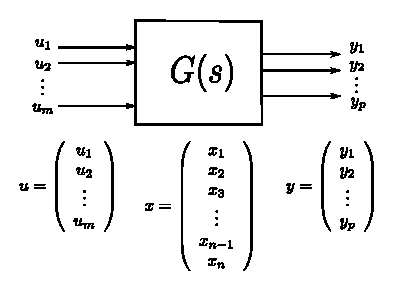
\includegraphics[width=0.6\linewidth]{sfigure/MIMO.eps}
\vspace{1cm}

$G(s)$:制御対象，$x \in {\mathbb R}^n$:状態, $ u \in {\mathbb R}^m $:入力, $ y \in {\mathbb R}^p $:出力
\end{center}


\end{frame}
%%%%%%%%%%%%%%%%%%%%%%%%%%%%%%%%%%%%%%%%%%%%%%%%%%%%%%%%%%%%%%%
\begin{frame}[t]
\frametitle{1.1 状態方程式（行列のサイズ）}
%-------------------------------------------------------------
\begin{center}
  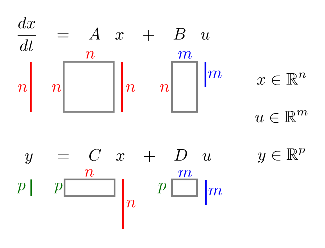
\includegraphics[width=0.7\linewidth]{sfigure/stateeq.eps}
\end{center}
\end{frame}



%%%%%%%%%%%%%%%%%%%%%%%%%%%%%%%%%%%%%%%%%%%%%%%%%%%%%%%%%%%%%%%
\begin{frame}[t]
\frametitle{1.1 状態方程式（ばね・質量・ダンパー系）}
%-------------------------------------------------------------
例）バネ・質量・ダンパー系

\newcounter{fig:spring-mass-damp}                    %%%%
\setcounter{fig:spring-mass-damp}{\value{figure}}  %%%%

\vspace*{-5mm}


\begin{figure}[h]
 \begin{center}
  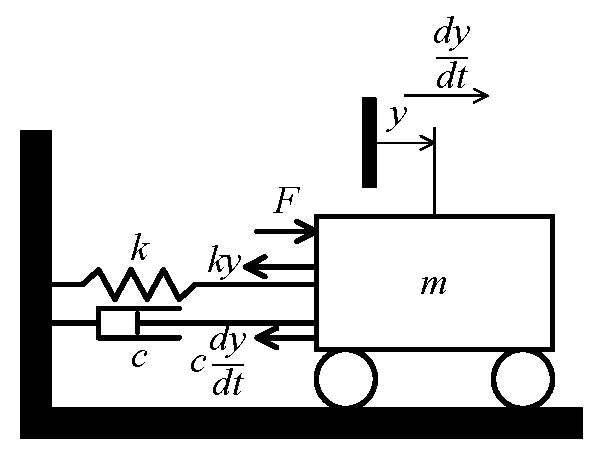
\includegraphics[width=0.35\linewidth]{sfigure/car1.eps}
  \caption{バネ・質量・ダンパー系}
  \label{fig_mass}
 \end{center}
\end{figure}

\vspace*{-5mm}


バネ・質量・ダンパー系の運動方程式：
\begin{gather}
 m \frac{d^2y}{dt^2} + c \frac{dy}{dt} + k y = F
 \hspace*{1cm}
 (\mbox{または}m \frac{d^2y}{dt^2} = F - k y - c \frac{dy}{dt})
\end{gather}
$k:$ バネ定数，$m:$ 質量，$c:$ ダンパーの粘性係数，\\
$y:$ 質量の変位（出力）,$F:$ 外力（入力）


\end{frame}

%%%%%%%%%%%%%%%%%%%%%%%%%%%%%%%%%%%%%%%%%%%%%%%%%%%%%%%%%%%%%%%
\begin{frame}[t]
\frametitle{1.1 状態方程式（ばね・質量・ダンパー系）}
%-------------------------------------------------------------
機械系での定石：システムの状態を「位置（角度）」「速度（角速度）」とする
\[
 \mbox{状態} =
 \left(\begin{array}{c}
         \mbox{位置}\\
   \mbox{速度}
       \end{array}\right)
\]
すなわち，
\begin{gather}
 x = \left(\begin{array}{c}
            x_1 \\
      x_2
     \end{array}\right)
 \defeq
 \left(\begin{array}{c}
         y \\
  \frac{dy}{dt}
       \end{array}\right)
\end{gather}
と定義すれば
\begin{columns}[t]
\begin{column}{0.4\textwidth}
\begin{align}
  \frac{dx_1}{dt} &= \frac{dy}{dt} \nonumber \\
                  &= x_2
\end{align}
\end{column}
\begin{column}{0.05\textwidth}

\end{column}
\begin{column}{0.5\textwidth}
\begin{align}
  \frac{dx_2}{dt} &= \frac{d}{dt} \left\{\frac{dy}{dt} \right\}
       = \frac{d^2 y}{dt^2} \nonumber \\
      &= \frac{1}{m} (-c \frac{dy}{dt} -k y + F) \nonumber \\
      &= -\frac{k}{m} x_1 - \frac{c}{m} x_2 + \frac{1}{m} F
\end{align}
\end{column}
\begin{column}{0.05\textwidth}

\end{column}
\end{columns}

\end{frame}

%%%%%%%%%%%%%%%%%%%%%%%%%%%%%%%%%%%%%%%%%%%%%%%%%%%%%%%%%%%%%%%
\begin{frame}[t]
\frametitle{1.1 状態方程式（ばね・質量・ダンパー系）}
%-------------------------------------------------------------
\vspace*{-5mm}
\setcounter{eqncountersave}{\value{equation}} %%%式カウンターsave
\addtocounter{equation}{-2} %%%%
\begin{columns}[t]
\begin{column}{0.4\textwidth}
\begin{align}
  \frac{dx_1}{dt} &= x_2
\end{align}
\end{column}
\begin{column}{0.05\textwidth}

\end{column}
\begin{column}{0.5\textwidth}
\begin{align}
  \frac{dx_2}{dt} &= -\frac{k}{m} x_1 - \frac{c}{m} x_2 + \frac{1}{m} F
\end{align}
\end{column}
\begin{column}{0.05\textwidth}

\end{column}
\end{columns}
%\end{block}
\ \\[5mm]
\setcounter{equation}{\value{eqncountersave}} %%%% 式カウンター復活

これらをまとめて
\begin{align}
 \frac{d}{dt} \left(\begin{array}{c}
               x_1 \\
         x_2
        \end{array}\right)
 &=
 \left(\begin{array}{cc}
        0            &         1     \\
  -\frac{k}{m} & - \frac{c}{m}
       \end{array}\right)
 \left(\begin{array}{c}
  x_1 \\
  x_2
       \end{array}\right)
 +
 \left(\begin{array}{c}
        0 \\
  \frac{1}{m}
       \end{array}\right)
 F \label{eq:massstate} \\
 y &=
 \left(\begin{array}{cc}
             1 & 0
       \end{array}\right)
 \left(\begin{array}{c}
        x_1 \\
  x_2
       \end{array}\right) \label{eq:massoutput}
\end{align}
と状態方程式で表わされる．
\end{frame}

%%%%%%%%%%%%%%%%%%%%%%%%%%%%%%%%%%%%%%%%%%%%%%%%%%%%%%%%%%%%%%%
\begin{frame}[t]
\frametitle{1.1 状態方程式（2質量系）}
%-------------------------------------------------------------
状態方程式は\Blue{\bf 多入出力系も容易に扱うこと
ができる}．\vspace{3mm}

例）2質量系

2つの質量間のバネ定数を$k$, 質量をそれぞれ$m_1$, $m_2$,
質量の平衡点からの変位をそれぞれ$y_1$, $y_2$,
外力をそれぞれ$F_1$, $F_2$として，運動方程式を表すと，
\begin{align}
 m_1 \frac{d^2y_1}{dt^2} - k (y_2 - y_1) &= F_1 \\
 m_2 \frac{d^2y_2}{dt^2} + k (y_2 - y_1) &= F_2
\end{align}

\begin{figure}[t]
 \begin{center}
  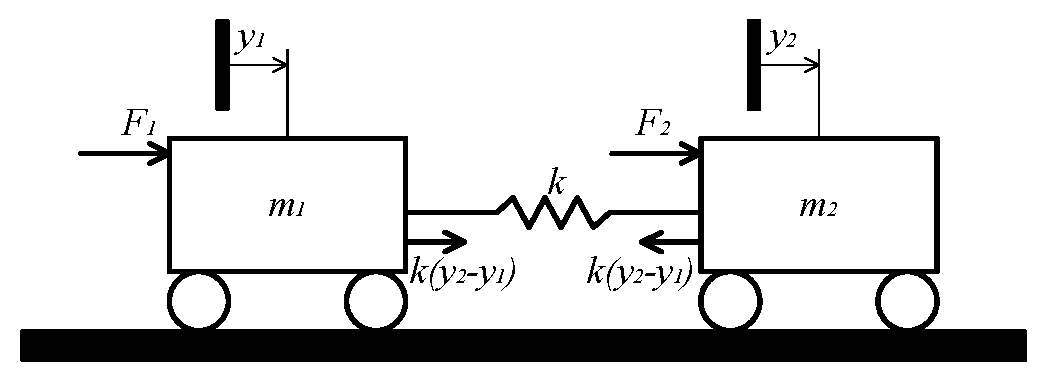
\includegraphics[width=0.6\linewidth]{sfigure/car2.eps}
  \caption{2質量系}
  \label{fig:spring-2mass}
 \end{center}
\end{figure}
\end{frame}

%%%%%%%%%%%%%%%%%%%%%%%%%%%%%%%%%%%%%%%%%%%%%%%%%%%%%%%%%%%%%%%
\begin{frame}[t]
\frametitle{1.1 状態方程式（2質量系）}
%-------------------------------------------------------------
\vspace*{-5mm}
\setcounter{eqncountersave}{\value{equation}} %%%%式カウンターsave
\addtocounter{equation}{-2} %%%%
\begin{align}
 m_1 \frac{d^2y_1}{dt^2} - k (y_2 - y_1) &= F_1 \\
 m_2 \frac{d^2y_2}{dt^2} + k (y_2 - y_1) &= F_2
\end{align}
\setcounter{equation}{\value{eqncountersave}} %%%%式カウンター復活

ここで，バネ・質量・ダンパー系と同様に，位置と速度を状態とすれば，以下の状態方程式で表される．
\begin{align}
 \frac{d}{dt} \left(\begin{array}{c}
               y_1 \\
         y_2 \\
         \frac{dy_1}{dt} \\
         \frac{dy_2}{dt}
        \end{array}\right)
 &=
 \left(\begin{array}{cccc}
        0 & 0 & 1 & 0     \\
        0 & 0 & 0 & 1     \\
  -\frac{k}{m_1} & \frac{k}{m_1} & 0 & 0 \\
  \frac{k}{m_2} & -\frac{k}{m_2} & 0 & 0 \\
       \end{array}\right)
 \left(\begin{array}{c}
        y_1 \\
  y_2 \\
  \frac{dy_1}{dt} \\
  \frac{dy_2}{dt}
       \end{array}\right)
 +
 \left(\begin{array}{cc}
        0 & 0 \\
        0 & 0 \\
  \frac{1}{m_1} & 0 \\
  0 & \frac{1}{m_2} \\
       \end{array}\right)
 \left(\begin{array}{c}
        F_1 \\
  F_2
       \end{array}\right) \\
 \left(\begin{array}{c}
        y_1 \\
  y_2
       \end{array}\right)
 &=
 \left(\begin{array}{cccc}
         1 & 0 & 0 & 0 \\
         0 & 1 & 0 & 0
       \end{array}\right)
 \left(\begin{array}{c}
        y_1 \\
  y_2 \\
  \frac{dy_1}{dt} \\
  \frac{dy_2}{dt}
       \end{array}\right)
\end{align}

\end{frame}

%%%%%%%%%%%%%%%%%%%%%%%%%%%%%%%%%%%%%%%%%%%%%%%%%%%%%%%%%%%%%%%
\begin{frame}[t]
\frametitle{1.1 状態方程式　＜演習＞ ３質量系の状態方程式}
%-------------------------------------------------------------
Fig.\ref{fig_3mass}の３質量系の状態方程式を求めよ．

\newcounter{fig:three-mass}                    %%%%
\setcounter{fig:three-mass}{\value{figure}}  %%%%

\begin{figure}[htbp]
 \begin{center}
  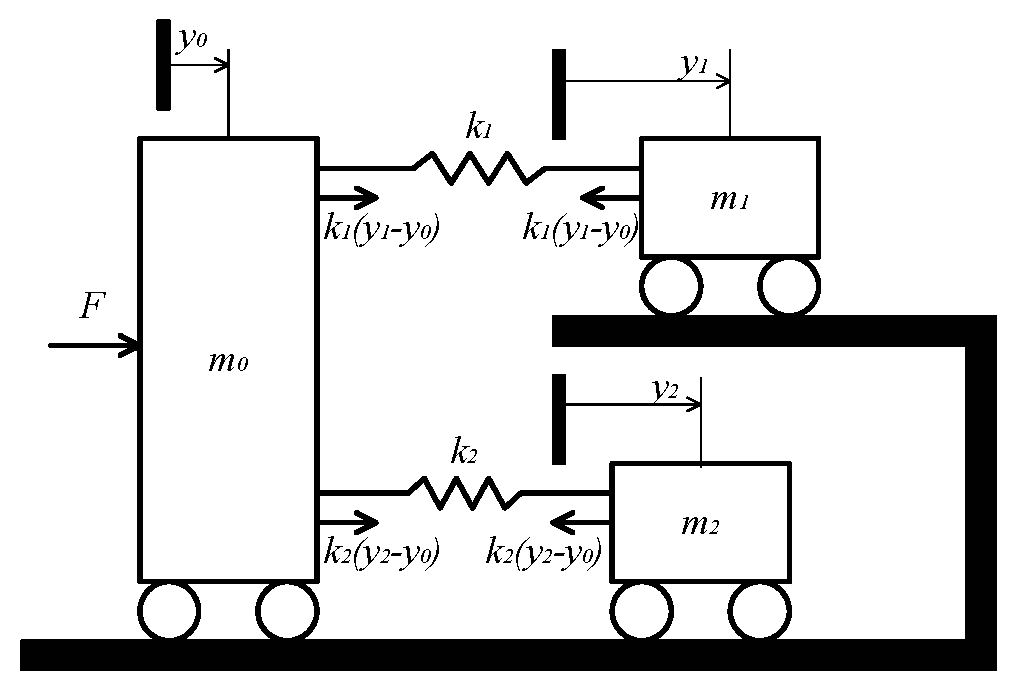
\includegraphics[width=0.45\linewidth]{sfigure/car3.eps}
  \caption{３質量系}
  \label{fig_3mass}
 \end{center}
\end{figure}

\noindent

(hint) 3質量系の運動方程式は以下であらわされる．（$\ddot{y}=\frac{d^2y}{dt^2}$）
\begin{align}
  m_0 \ddot{y}_0 & = F + k_1 (y_1 - y_0) + k_2 (y_2-y_0)
\nonumber \\
  m_1 \ddot{y}_1 & = - k_1 (y_1 - y_0)
\nonumber \\
  m_2 \ddot{y}_2 & = - k_2 (y_2 - y_0)
\nonumber
\end{align}
\end{frame}

%%%%%%%%%%%%%%%%%%%%%%%%%%%%%%%%%%%%%%%%%%%%%%%%%%%%%%%%%%%%%%%
\begin{frame}[t]
\frametitle{1.1 状態方程式（RC回路）}
%-------------------------------------------------------------
電気回路は$C$の電圧，$L$の電流を状態とすると状態方程式が求められる．
\begin{figure}[htbp]
 \begin{center}
  \includegraphics[width=0.4\linewidth]{sfigure/RC.eps}
  \caption{RC回路}
  \label{fig_RC}

 \end{center}
\end{figure}

例えばFig. \ref{fig_RC}の回路（入力:$v_i$, 出力:$v_o$）の方程式は
\begin{align*}
  v_R &= i R, \ \
  i  = C \frac{d v_C}{dt}, \ \
  v_i  = v_R + v_C, \ \
  v_o  = v_C
\end{align*}
となるが，状態を$v_C$（$C$の電圧）として，その微分を整理することにより以下の状態方程式が得られる．
\begin{align*}
  \frac{d v_C}{dt}
  &= \frac{i}{C}
  = \frac{v_R/R}{C}
  = \frac{v_R}{RC}
  = \frac{v_i - v_C}{RC}
  = - \frac{1}{RC} v_C + \frac{1}{RC} v_i \\
  v_o & = v_C
\end{align*}
\end{frame}

%%%%%%%%%%%%%%%%%%%%%%%%%%%%%%%%%%%%%%%%%%%%%%%%%%%%%%%%%%%%%%%
\begin{frame}[t]
\frametitle{1.1 状態方程式（LR回路）}
%-------------------------------------------------------------
\begin{figure}[htbp]
 \begin{center}
  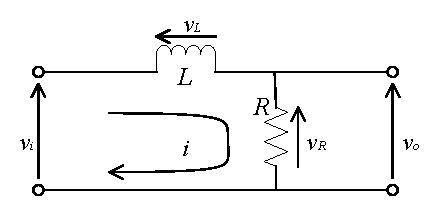
\includegraphics[width=0.4\linewidth]{sfigure/LR.eps}
  \caption{LR回路}
  \label{fig_LR}
 \end{center}
\end{figure}

また，Fig. \ref{fig_LR}の回路の方程式は
\begin{align*}
  v_L & = L \frac{d i}{dt}, \ \
  v_R = i R, \ \
  v_i  = v_L + v_R, \ \
  v_o  = v_R
\end{align*}
であり，状態を$i$（$L$の電流）として，その微分を整理することにより以下の状態方程式が得られる．
\begin{align*}
  \frac{d i}{dt}
  &= \frac{v_L}{L}
  = \frac{v_i - v_R}{L}
  = - \frac{1}{L} v_R + \frac{1}{L} v_i
  = - \frac{1}{L} R i + \frac{1}{L} v_i
  = - \frac{R}{L} i + \frac{1}{L} v_i \\
  v_o & = v_R = R i
\end{align*}
\end{frame}

%%%%%%%%%%%%%%%%%%%%%%%%%%%%%%%%%%%%%%%%%%%%%%%%%%%%%%%%%%%%%%%
\begin{frame}[t]
\frametitle{1.1 状態方程式　＜演習＞ LCR回路の状態方程式}
%-------------------------------------------------------------
以下の電気回路の状態方程式を求めよ（入力:$v_i$, 出力:$v_o$）．

\begin{figure}[htbp]
 \begin{center}
  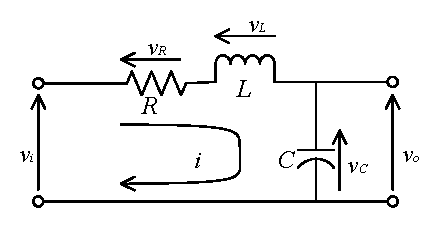
\includegraphics[width=0.4\linewidth]{sfigure/LCR.eps}
  \caption{LCR回路}
  \label{fig_LCR}
 \end{center}
\end{figure}

\noindent
(hint)電気回路は$C$の電圧，$L$の電流を状態とすると状態方程式が求められる．
また，このLCR回路の方程式は以下で与えられる．
\begin{align*}
  v_L & = L \frac{d i}{dt}, \ \
  i  = C \frac{d v_C}{dt}, \ \
  v_R = i R  \\
  v_i  &= v_L + v_C + v_R, \ \
  v_o  = v_C
\end{align*}
\end{frame}


%%%%%%%%%%%%%%%%%%%%%%%%%%%%%%%%%%%%%%%%%%%%%%%%%%%%%%%%%%%%%%%
\begin{frame}[t]
\frametitle{1.2 座標変換（座標変換の定義）}
%-------------------------------------------------------------
状態方程式
\begin{align}
   \frac{dx}{dt} &= A x(t) + B u(t) \tag{\ref{state_eq}} \\
 y(t) &= C x(t) + D u(t) \tag{\ref{output_eq}}
\end{align}
システム(\ref{state_eq})(\ref{output_eq})における状態$x$はシステムの内部状
態を表わすもので，システムの入出力に直接には現われない．そこで，この状態
$x$を次のような{\bf {座標変換}(coordinate transformation)}で$\bar{x}$に変換することを考える．
\begin{equation}
 x = T \bar{x} \quad (\bar{x} = T^{-1}x)
\end{equation}
ここで$T$は正則な行列(nonsingular)であるとする．

\end{frame}

%%%%%%%%%%%%%%%%%%%%%%%%%%%%%%%%%%%%%%%%%%%%%%%%%%%%%%%%%%%%%%%
\begin{frame}[t]
\frametitle{1.2 座標変換（座標変換と状態方程式）}
%-------------------------------------------------------------
状態$\bar{x}$を時間微分(time derivative)すれば
\begin{align}
 \frac{d \bar{x}}{dt} &= T^{-1} \frac{dx}{dt} \nonumber \\
 &= T^{-1} ( A x + B u) \nonumber \\
 &= T^{-1} A T \bar{x} + T^{-1} B u \nonumber \\
 & \defeq \bar{A} \bar{x} + \bar{B} u
\label{eq:anotherstate_st}
\end{align}
なる状態方程式を得る．また出力方程式(output equation)は
\begin{align}
 y &= C T \bar{x} + D u \nonumber \\
   & \defeq \bar{C} \bar{x} + \bar{D} u
\label{eq:anotherstate_out}
\end{align}
となる．このように座標変換によりシステムの状態を変えても状態方程式でシス
テムの挙動を表わすことができる．
\end{frame}

%%%%%%%%%%%%%%%%%%%%%%%%%%%%%%%%%%%%%%%%%%%%%%%%%%%%%%%%%%%%%%%
\begin{frame}[t]
\frametitle{1.3 状態方程式から伝達関数へ（伝達関数）}
%-------------------------------------------------------------
状態方程式
\begin{align}
 \frac{dx}{dt} &= A x(t) + B u(t) \tag{\ref{state_eq}} \\
 y(t) &= C x(t) + D u(t) \tag{\ref{output_eq}}
\end{align}

状態方程式(\ref{state_eq})において，
状態$x$, 入力$u$のラプラス変換を，
\begin{align}
 {\cal L}(x(t)) &=
 {\cal L} \left(
        \begin{array}{c}
	 x_1(t) \\
	 x_2(t)
	\end{array}
	\right) =
 \left(
 \begin{array}{c}
  {\cal L}(x_1(t)) \\
  {\cal L}(x_2(t))
 \end{array}
 \right) =
 \left(
 \begin{array}{c}
  X_1(s) \\
  X_2(s)
 \end{array}
 \right) = X(s) \\
 {\cal L}(u(t)) &= U(s)
\end{align}
とする．これを用いて
(\ref{state_eq})をラプラス変換し，$x$の初期値を$x(0) = 0$とおけば
\begin{eqnarray*}
 s X(s) = A X(s) + B U(s) & \Leftrightarrow & s X(s) - A X(s) = B U(s) \\
                          & \Leftrightarrow & (sI - A)X(s) = B U(s)
\end{eqnarray*}
\begin{equation}
 \therefore X(s) = (s I - A)^{-1} B U(s)
\end{equation}
を得る．
\end{frame}

%%%%%%%%%%%%%%%%%%%%%%%%%%%%%%%%%%%%%%%%%%%%%%%%%%%%%%%%%%%%%%%
\begin{frame}[t]
\frametitle{1.3 状態方程式から伝達関数へ(伝達関数)}
%-------------------------------------------------------------
状態方程式
\begin{align}
   \frac{dx}{dt} &= A x(t) + B u(t) \tag{\ref{state_eq}} \\
 y(t) &= C x(t) + D u(t) \tag{\ref{output_eq}}
\end{align}

同様に，
出力方程式(\ref{output_eq})を考えれば入力から出力までの伝達関数(transfer function)$G(s)$は
\begin{align}
 Y(s) &= C X(s) + D U(s) \nonumber \\
      &= C (s I - A)^{-1} B U(s) + D U(s) \nonumber \\
      &= \{ C ( s I - A )^{-1} B + D \} U(s) \\
      &\defeq G(s) U(s)
\end{align}
で表わされる．
\end{frame}

%%%%%%%%%%%%%%%%%%%%%%%%%%%%%%%%%%%%%%%%%%%%%%%%%%%%%%%%%%%%%%%
\begin{frame}[t]
\frametitle{1.3 状態方程式から伝達関数へ{\small （バネ・質量・ダンパー系）}}
%-------------------------------------------------------------
例）バネ・質量・ダンパー系
\setcounter{countersave}{\value{figure}} %%%%式カウンターsave
\setcounter{figure}{\value{fig:spring-mass-damp}}
\begin{figure}[h]
 \begin{center}
	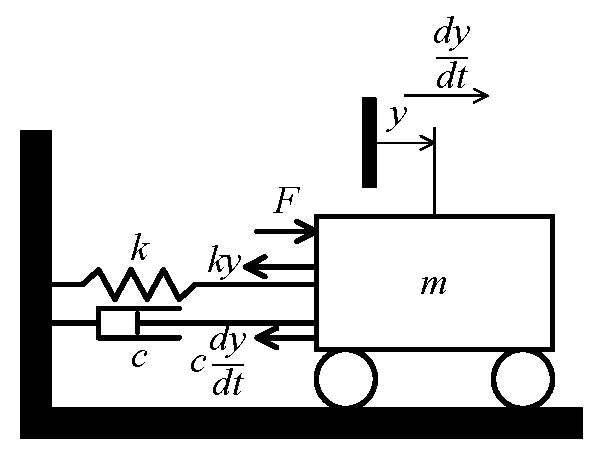
\includegraphics[width=0.35\linewidth]{sfigure/car1.eps}
  \caption{バネ・質量・ダンパー系}
 \end{center}
\end{figure}
\setcounter{figure}{\value{countersave}} %%%%式カウンター復活
バネ・質量・ダンパー系の状態方程式：
\begin{align}
 \frac{d}{dt} \left(\begin{array}{c}
	             x_1 \\
		     x_2
		    \end{array}\right)
 &=
 \left(\begin{array}{cc}
        0            &         1     \\
	-\frac{k}{m} & - \frac{c}{m}
       \end{array}\right)
 \left(\begin{array}{c}
	x_1 \\
	x_2
       \end{array}\right)
 +
 \left(\begin{array}{c}
        0 \\
	\frac{1}{m}
       \end{array}\right)
 F \tag{\ref{eq:massstate}}\\
 y &=
 \left(\begin{array}{cc}
             1 & 0
       \end{array}\right)
 \left(\begin{array}{c}
        x_1 \\
	x_2
       \end{array}\right)  \tag{\ref{eq:massoutput}}
\end{align}
\end{frame}

%%%%%%%%%%%%%%%%%%%%%%%%%%%%%%%%%%%%%%%%%%%%%%%%%%%%%%%%%%%%%%%
\begin{frame}[t]
\frametitle{1.3 状態方程式から伝達関数へ{\small （バネ・質量・ダンパー系）}}
%-------------------------------------------------------------
状態方程式(\ref{eq:massstate})(\ref{eq:massoutput})で表された
バネ・質量・ダンパー系の伝達関数は
以下のように計算できる．
\begin{align}
 G(s)
 &= C (s I - A)^{-1} B \\
 &= \left(
     \begin{array}{cc}
      1 & 0
     \end{array}
    \right)
    \left(
     \begin{array}{cc}
      s           & -1 \\
      \frac{k}{m} & s+\frac{c}{m}
     \end{array}
    \right)^{-1}
    \left(
     \begin{array}{c}
      0 \\
      \frac{1}{m}
     \end{array}
    \right) \nonumber \\
 &= \left(
     \begin{array}{cc}
      1 & 0
     \end{array}
    \right)
    \left\{
     \frac{1}{s(s + \frac{c}{m})+\frac{k}{m}}
     \left(
     \begin{array}{cc}
      s+\frac{c}{m} & 1 \\
      -\frac{k}{m}  & s
     \end{array}
     \right)
    \right\}
    \left(
     \begin{array}{c}
      0 \\
      \frac{1}{m}
     \end{array}
    \right) \nonumber \\
 &= \frac{1}{s^2 + \frac{c}{m}s + \frac{k}{m}}
    \left(
     \begin{array}{cc}
      1 & 0
     \end{array}
    \right)
    \left(
     \begin{array}{cc}
      s+\frac{c}{m} & 1 \\
      -\frac{k}{m}  & s
     \end{array}
    \right)
    \left(
     \begin{array}{c}
      0 \\
      \frac{1}{m}
     \end{array}
    \right) \nonumber \\
 &= \frac{1}{s^2 + \frac{c}{m}s + \frac{k}{m}}
    \left(
     \begin{array}{cc}
      1 & 0
     \end{array}
    \right)
    \left(
     \begin{array}{c}
      \frac{1}{m} \\
      \frac{s}{m}
     \end{array}
    \right) \nonumber \\
 &= \frac{\frac{1}{m}}{s^2 + \frac{c}{m}s + \frac{k}{m}}
\end{align}
\end{frame}

%%%%%%%%%%%%%%%%%%%%%%%%%%%%%%%%%%%%%%%%%%%%%%%%%%%%%%%%%%%%%%%
\begin{frame}[t]
\frametitle{1.3 状態方程式から伝達関数へ{\small （座標変換後の伝達関数）}}
%-------------------------------------------------------------
座標変換されたシステム
\begin{align}
 \frac{d \bar{x}}{dt}
 &= T^{-1} A T \bar{x} + T^{-1} B u \nonumber \\
 & \defeq \bar{A} \bar{x} + \bar{B} u \tag{\ref{eq:anotherstate_st}}\\
 y &= C T \bar{x} + D u \nonumber \\
   & \defeq \bar{C} \bar{x} + \bar{D} u
\tag{\ref{eq:anotherstate_out}}
\end{align}
の伝達関数は座標変換される前の伝達関数と等しくなる．

(証明)
\begin{align}
 \bar{C} (sI - \bar{A})^{-1} \bar{B} + \bar{D}
 &= CT (sI - T^{-1} A T )^{-1} T^{-1} B + D
\nonumber\\
 &= C T \{ T^{-1} (sI - A) T \}^{-1} T^{-1} B + D
\nonumber\\
 &= C T \{ T^{-1} (sI - A)^{-1} T \} T^{-1} B + D
\nonumber \\
 &= C (sI - A)^{-1} B + D
\end{align}
\end{frame}

%%%%%%%%%%%%%%%%%%%%%%%%%%%%%%%%%%%%%%%%%%%%%%%%%%%%%%%%%%%%%%%
\begin{frame}[t]
\frametitle{1.4 1入出力伝達関数から状態方程式へ(1入出力)}
%-------------------------------------------------------------
\Blue{\bf {一入出力}(SISO: single input single output)}の伝達関数：
\begin{equation}
 G(s) =
  \frac{b_{n-1} s^{n-1} + b_{n-2} s^{n-2} + \cdots + b_1 s + b_0}
  {s^n + a_{n-1} s^{n-1} + a_{n-2} s^{n-2} + \cdots + a_1 s + a_0}
  + d
  \label{eq:G(s)}
\end{equation}
伝達関数\eqref{eq:G(s)} で表わされるシステムの状態空間表現は一意ではない（座標変換分の自由度がある）．
\end{frame}


%%%%%%%%%%%%%%%%%%%%%%%%%%%%%%%%%%%%%%%%%%%%%%%%%%%%%%%%%%%%%%%
\begin{frame}[t]
\frametitle{1.4 1入出力伝達関数から状態方程式へ{\small （可制御正準系）}}
%-------------------------------------------------------------
\Blue{\bf {可制御正準形}(controller canonical form)}
\begin{align}
 \frac{d}{dt}
  \left(\begin{array}{c}
         x_1 \\
	 x_2 \\
	 \vdots \\
	 x_{n-1} \\
	 x_n
	\end{array}\right)
  &=
  \left(\begin{array}{ccccc}
     0      & 1      & 0      & \cdots & 0 \\
	 0      & 0      & 1      & \ddots & \vdots \\
	 \vdots & \vdots & \ddots & \ddots & 0 \\
	 0      & 0      & \cdots & 0      & 1 \\
	 -a_0   & -a_1   & \cdots & -a_{n-2} & -a_{n-1}
	\end{array}\right)
  \left(\begin{array}{c}
	 x_1 \\
	 x_2 \\
	 \vdots \\
	 x_{n-1} \\
	 x_n
	\end{array}\right)
  +
  \left(\begin{array}{c}
         0 \\
	 0 \\
	 \vdots \\
	 0 \\
	 1
	\end{array}\right)
  u \label{eq:canoform}\\
y &=
 \left(\begin{array}{ccccc}
        b_0 & b_1 & \cdots & b_{n-2} & b_{n-1}
       \end{array}\right)
 \left(\begin{array}{c}
        x_1 \\
	x_2 \\
	\vdots \\
	x_{n-1} \\
	x_n
       \end{array}\right)
 + d u
\end{align}

1 入出力伝達関数(\ref{eq:G(s)})は可制御正準形で表される．
\end{frame}

%%%%%%%%%%%%%%%%%%%%%%%%%%%%%%%%%%%%%%%%%%%%%%%%%%%%%%%%%%%%%%%
\begin{frame}[t]
\frametitle{1.4 1入出力伝達関数から状態方程式へ{\small （可制御正準系の証明）}}
%-------------------------------------------------------------
1 入出力伝達関数(\ref{eq:G(s)})は可制御正準形で表されることの証明:

まず，可制御正準系の$(sI-A)^{-1}$ は
\begin{align}
 (sI-A)^{-1}
 &=
    \left(\begin{array}{ccccc}
     s      & -1     &  0     & \cdots &  0 \\
	 0      &  s     & -1     & \ddots &  \vdots \\
	 \vdots & \vdots & \ddots & \ddots &  0 \\
	 0      &  0     & \cdots & s      & -1 \\
	 a_0    &  a_1   & \cdots & a_{n-2}  &  s+a_{n-1}
	\end{array}\right)^{-1}
\nonumber\\
 &=
    \frac{1}{s^n + a_{n-1} s^{n-1}  + \cdots + a_0}
    \left(\begin{array}{ccccc}
        &    &        &    &  1 \\
	    &    &        &    &  s \\
	  * &  * & \cdots &  * &  \vdots \\
	    &    &        &    &  s^{n-2} \\
	    &    &        &    &  s^{n-1}
	\end{array}\right) \label{eq:lemma_inverse}
\end{align}
となることを示す．
\end{frame}

%%%%%%%%%%%%%%%%%%%%%%%%%%%%%%%%%%%%%%%%%%%%%%%%%%%%%%%%%%%%%%%
\begin{frame}[t]
\frametitle{1.4 1入出力伝達関数から状態方程式へ{\small （可制御正準系の証明）}}
%-------------------------------------------------------------
等式\eqref{eq:lemma_inverse} が成り立つことは$(sI-A)(sI-A)^{-1}=I$より
\begin{align}
    \left(\begin{array}{ccccc}
     s      & -1     &  0     & \cdots &  0 \\
	 0      &  s     & -1     & \ddots &  \vdots \\
	 \vdots & \vdots & \ddots & \ddots &  0 \\
	 0      &  0     & \cdots & s      & -1 \\
	 a_0    &  a_1   & \cdots & a_{n-2}  &  s+a_{n-1}
	\end{array}\right)
  &
    \left(\begin{array}{ccccc}
        &    &        &    &  1 \\
	    &    &        &    &  s \\
	  * &  * & \cdots &  * &  \vdots \\
	    &    &        &    &  s^{n-2} \\
	    &    &        &    &  s^{n-1}
	\end{array}\right) \nonumber \\
    \frac{1}{s^n + a_{n-1} s^{n-1}  + \cdots + a_0}
 &=
    \left(\begin{array}{ccccc}
        &    &        &    &  0 \\
	    &    &        &    &  0 \\
	  * &  * & \cdots &  * &  \vdots \\
	    &    &        &    &  0 \\
	    &    &        &    &  1
	\end{array}\right)
\end{align}
となることから明らかである．
\end{frame}

%%%%%%%%%%%%%%%%%%%%%%%%%%%%%%%%%%%%%%%%%%%%%%%%%%%%%%%%%%%%%%%
\begin{frame}[t]
\frametitle{1.4 1入出力伝達関数から状態方程式へ{\small （可制御正準系の証明）}}
%-------------------------------------------------------------
よって，可制御正準系の伝達関数は
{\tiny
\begin{align}
 C(sI-A)^{-1}B + D
 &=
 \frac{
    \left(\begin{array}{ccccc}
        b_0 & b_1 & \cdots & b_{n-2} & b_{n-1}
    \end{array}\right)
    \left(\begin{array}{ccccc}
        &    &        &    &  1 \\
	    &    &        &    &  s \\
	  * &  * & \cdots &  * &  \vdots \\
	    &    &        &    &  s^{n-2} \\
	    &    &        &    &  s^{n-1}
	\end{array}\right)
    \left(\begin{array}{c}
         0 \\
	 0 \\
	 \vdots \\
	 0 \\
	 1
	\end{array}\right)
 }
 {s^n + a_{n-1} s^{n-1}  + \cdots + a_0}
    + d
\nonumber\\[1cm]
 &=
 \frac{
    \left(\begin{array}{ccccc}
        b_0 & b_1 & \cdots & b_{n-2} & b_{n-1}
    \end{array}\right)
    \left(\begin{array}{c}
     1 \\
	 s \\
	 \vdots \\
	 s^{n-2} \\
	 s^{n-1}
	\end{array}\right)
 }
 {s^n + a_{n-1} s^{n-1}  + \cdots + a_0}
    + d
\nonumber \\[1cm]
 &=
   \frac{b_{n-1} s^{n-1} + b_{n-2} s^{n-2} + \cdots + b_1 s + b_0}
  {s^n + a_{n-1} s^{n-1} + a_{n-2} s^{n-2} + \cdots + a_1 s + a_0}
  + d
\end{align}
}
となる．(証明終了)
\end{frame}

%%%%%%%%%%%%%%%%%%%%%%%%%%%%%%%%%%%%%%%%%%%%%%%%%%%%%%%%%%%%%%
\begin{frame}[t]
\frametitle{1.4 1入出力伝達関数から状態方程式へ{ (近似微分要素)}}
%-------------------------------------------------------------
例として，近似微分要素を表す伝達関数について確認する．
\begin{align}
 \frac{Ts}{Ts+1} = \frac{s}{s+\frac{1}{T}}
 = \frac{-\frac{1}{T}}{s+\frac{1}{T}} + 1
\end{align}
となるので，状態方程式で表すと
\begin{align}
 \frac{dx}{dt} &= -\frac{1}{T} x + 1u \\
 y             &= -\frac{1}{T} x + 1u
\end{align}
となる．
\end{frame}

%%%%%%%%%%%%%%%%%%%%%%%%%%%%%%%%%%%%%%%%%%%%%%%%%%%%%%%%%%%%%%
\begin{frame}[t]
\frametitle{1.5 可制御性 (定義)}
%-------------------------------------------------------------
状態方程式
\begin{align}
 \frac{dx}{dt} &= A x(t) + B u(t) \tag{\ref{state_eq}} \\
 y(t) &= C x(t) + D u(t) \tag{\ref{output_eq}}
\end{align}

\begin{block}{可制御}
状態方程式(\ref{state_eq})において初期状態$x(0)=x_0$を有限時間$t_1$で原点に移す$(x(t_1)=0)$入力$u(t), t\in[0,t_1]$が存在するとき$x_0$は\Blue{\bf 可制御(controllable)}であるという．
また，すべての状態$x_0$が可制御であるとき，状態方程式は可制御であるという．
\end{block}

可制御でない状態方程式は\Blue{\bf 不可制御(uncontrollable)}であるという．

可制御性は$A,B$行列のみに依存する性質なので\Blue{\bf $(A,B)$可制御}ということもある．
\end{frame}



%%%%%%%%%%%%%%%%%%%%%%%%%%%%%%%%%%%%%%%%%%%%%%%%%%%%%%%%%%%%%%
\begin{frame}[t]
\frametitle{1.5 可制御性 (（行列論：復習）ランク)}
%-------------------------------------------------------------
\Blue{\bf 行列の階数($\rank$)}:与えられた行列における独立な列ベクトル(行ベクトル)の数．

(例)
\[
 \begin{array}{lcl}
  \rank
   \left(
    \begin{array}{cc}
     1 & 0 \\
     0 & 1 \\
     0 & 0
    \end{array}
   \right) = 2 & \Rightarrow & \mbox{1列目と2列目は独立なベクトル} \\
  \rank
   \left(
    \begin{array}{cc}
     1 & 2 \\
     0 & 0 \\
     0 & 0
    \end{array}
   \right) = 1 & \Rightarrow & \mbox{2列目は1列目を2倍したベクトル} \\
  \rank
   \left(
    \begin{array}{ccc}
     1 & 0 & 1 \\
     0 & 1 & 1\\
     0 & 0 & 0
    \end{array}
   \right) = 2 & \Rightarrow & \mbox{3列目は1列目と2列目の線形結合}
 \end{array}
\]
\end{frame}

%%%%%%%%%%%%%%%%%%%%%%%%%%%%%%%%%%%%%%%%%%%%%%%%%%%%%%%%%%%%%%
\begin{frame}[t]
\frametitle{1.5 可制御性 (（行列論：復習）ブロック行列)}
%-------------------------------------------------------------
ブロック行列：行列をブロックに分けて計算することがある．
\begin{equation*}
	A =
	\left(\begin{array}{ccc}
			a_{11} & a_{12} & a_{13}\\
			a_{21} & a_{22} & a_{23}\\
			a_{31} & a_{32} & a_{33}\\
			a_{41} & a_{42} & a_{43}
	\end{array}\right)
	=
	\left(\begin{array}{c|cc}
			a_{11} & a_{12} & a_{13}\\
			a_{21} & a_{22} & a_{23}\\
			\hline
			a_{31} & a_{32} & a_{33}\\
			a_{41} & a_{42} & a_{43}
	\end{array}\right)
	=
	\left(\begin{array}{cc}
		A_{11} & A_{12} \\
		A_{21} & A_{22}
	\end{array}\right)
\end{equation*}

ブロック行列の積：通常の行列と同様に計算できる．
\begin{equation*}
	\left(\begin{array}{cc}
		A_{11} & A_{12} \\
		A_{21} & A_{22}
	\end{array}\right)
	\left(\begin{array}{cc}
		B_{11} & B_{12} \\
		B_{21} & B_{22} \\
	\end{array}\right)
	=
	\left(\begin{array}{cc}
		A_{11} B_{11} + A_{12} B_{21} & A_{11} B_{12} + A_{12} B_{22} \\
		A_{21} B_{11} + A_{22} B_{21} & A_{21} B_{12} + A_{22} B_{22}
	\end{array}\right)
\end{equation*}
　　それぞれの行列の積と和が計算できるサイズのときのみ成立(例)
\begin{equation*}
	\left(\begin{array}{c|cc}
			a_{11} & a_{12} & a_{13}\\
			a_{21} & a_{22} & a_{23}\\
			\hline
			a_{31} & a_{32} & a_{33}\\
			a_{41} & a_{42} & a_{43}
	\end{array}\right)
	\left(\begin{array}{cc|c}
			b_{11} & b_{12} & b_{13}\\
			\hline
			b_{21} & b_{22} & b_{23}\\
			b_{31} & b_{32} & b_{33}
	\end{array}\right)
\end{equation*}
\end{frame}


%%%%%%%%%%%%%%%%%%%%%%%%%%%%%%%%%%%%%%%%%%%%%%%%%%%%%%%%%%%%%%
\begin{frame}[t]
\frametitle{1.5 可制御性 (不可制御な状態方程式)}
%-------------------------------------------------------------

以下のシステムの状態の一部$x_2$が入力$u$の影響を受けない（制御できない）ための条件を考える．

\begin{align}
 \frac{d}{dt}
  \left(\begin{array}{c}
         {x}_1 \\
	 {x}_2
	\end{array}\right)
  &=
  \left(\begin{array}{cc}
         {A}_{11} & {A}_{12} \\
	     {A}_{21} & {A}_{22}
	\end{array}\right)
  \left(\begin{array}{c}
         {x}_1 \\
	 {x}_2
	\end{array}\right)
  +
  \left(\begin{array}{c}
         {B}_1 \\
	 {B}_2
	\end{array}\right)
  u \\
 y &=
  \left(\begin{array}{cc}
         {C}_1 & {C}_2
	\end{array}\right)
  \left(\begin{array}{c}
         {x}_1 \\
	 {x}_2
	\end{array}\right)
  + D u
\end{align}
ここで$x = \left(\begin{array}{c} {x}_1 \\ {x}_2 \end{array}\right) \in {\mathbb R}^n$,
$x_1 \in {\mathbb R}^r$, $x_2 \in {\mathbb R}^{n-r}$で，$A,B,C$行列は$x$の分割にあわせて定義されているものとする（例えば$A_{11} \in {\mathbb R}^{r \times r}$, $A_{12} \in {\mathbb R}^{r \times (n-r)}$など）．
このシステムを次のように書き下す．
\begin{align}
 \frac{dx_1}{dt} &= A_{11} x_1 + A_{12} x_2 + B_1 u
\label{eq:controllable01} \\
 \frac{dx_2}{dt} &= A_{21} x_1 + A_{22} x_2 + B_2 u
\label{eq:controllable02}
\end{align}
(\ref{eq:controllable02})において$dx_2/dt$が入力$u$の影響を受けないためには最低限$B_2=0$の必要がある．
\end{frame}

%%%%%%%%%%%%%%%%%%%%%%%%%%%%%%%%%%%%%%%%%%%%%%%%%%%%%%%%%%%%%%
\begin{frame}[t]
\frametitle{1.5 可制御性 (不可制御な状態方程式)}
%-------------------------------------------------------------

$B_2=0$とすると状態方程式は以下のようになる．


\begin{align}
 \frac{d}{dt}
  \left(\begin{array}{c}
         {x}_1 \\
	 {x}_2
	\end{array}\right)
  &=
  \left(\begin{array}{cc}
         {A}_{11} & {A}_{12} \\
	     {A}_{21} & {A}_{22}
	\end{array}\right)
  \left(\begin{array}{c}
         {x}_1 \\
	 {x}_2
	\end{array}\right)
  +
  \left(\begin{array}{c}
         {B}_1 \\
	 \Red{0}
	\end{array}\right)
  u \\
 y &=
  \left(\begin{array}{cc}
         {C}_1 & {C}_2
	\end{array}\right)
  \left(\begin{array}{c}
         {x}_1 \\
	 {x}_2
	\end{array}\right)
  + D u
\end{align}
このシステムを次のように書き下す．
\begin{align}
 \frac{dx_1}{dt} &= A_{11} x_1 + A_{12} x_2 + B_1 u
\label{eq:controllable1} \\
 \frac{dx_2}{dt} &= A_{21} x_1 + A_{22} x_2
\label{eq:controllable2}
\end{align}
(\ref{eq:controllable1})より，$x_1$は入力$u$の影響を受ける．(\ref{eq:controllable2})より$x_2$は直接は入力$u$の影響は受けないが，($u$の影響を受ける)$x_1$の影響を受けるので，間接的に入力$u$の影響を受けていることになる．
\end{frame}



%%%%%%%%%%%%%%%%%%%%%%%%%%%%%%%%%%%%%%%%%%%%%%%%%%%%%%%%%%%%%%
\begin{frame}[t]
\frametitle{1.5 可制御性 (不可制御な状態方程式)}
%-------------------------------------------------------------
しかし，もし状態方程式の$A_{21}$部分が$0$行列であるとすれば
\begin{align}
 \frac{d}{dt}
  \left(\begin{array}{c}
         {x}_1 \\
   {x}_2
  \end{array}\right)
  &=
  \left(\begin{array}{cc}
         {A}_{11} & {A}_{12} \\
       \Red{0}    & {A}_{22}
  \end{array}\right)
  \left(\begin{array}{c}
         {x}_1 \\
   {x}_2
  \end{array}\right)
  +
  \left(\begin{array}{c}
         {B}_1 \\
   0
  \end{array}\right)
  u
\label{eq:uncontrollable1}\\
 y &=
  \left(\begin{array}{cc}
         {C}_1 & {C}_2
  \end{array}\right)
  \left(\begin{array}{c}
         {x}_1 \\
   {x}_2
  \end{array}\right)
  + D u
\label{eq:uncontrollable2}\vspace{-2mm}
\end{align}
であり，書き下すと\vspace{-2mm}
\begin{align}
  \left\{
    \begin{alignedat}{3}
    \frac{d x_1}{dt} &= A_{11} x_1 +&& A_{12}x_2 + B_{1} u\\
    \frac{d x_2}{dt} &= &&A_{22}x_2
    \end{alignedat}
  \right. \label{eq:uncontrollable3}
\end{align}
となり，
\begin{itemize}
\item $x_2$は入力$u$の影響を受けない（制御できない）.

\item $x_2(0) \neq 0$の場合には有限時間$t_1$では$x_2(t_1)$は$0$にはならない.

\end{itemize}
つまり，状態方程式は不可制御である．
\begin{quote}
(\ref{eq:uncontrollable1})(\ref{eq:uncontrollable2})で表されるシステムや，座標変換で(\ref{eq:uncontrollable1})(\ref{eq:uncontrollable2})に変換されるシステムは不可制御なシステムである．
\end{quote}
\addtocounter{figure}{+1}
\end{frame}


%%%%%%%%%%%%%%%%%%%%%%%%%%%%%%%%%%%%%%%%%%%%%%%%%%%%%%%%%%%%%%
\begin{frame}[t]
\frametitle{1.5 可制御性 (不可制御な状態方程式)}
%-------------------------------------------------------------
  \begin{align}
    \begin{array}{cc}
      \left(
        \begin{array}{c}
          x_1 \\ x_2
        \end{array}
      \right)\in \mathbb{R}^{n} &
      \begin{aligned}
        x_1 \in& \mathbb{R}^r \\
        x_2 \in& \mathbb{R}^{n-r} \\
      \end{aligned}
    \end{array} \notag
  \end{align}
  \begin{align}
    \frac{d}{dt}
    \left(
      \begin{array}{c}
        x_1 \\ x_2
      \end{array}
    \right) = \left(
      \begin{array}{cc}
        A_{11} & A_{12} \\  \textcolor{red}{0} & A_{22}
      \end{array}
    \right)
    \left(
      \begin{array}{c}
        x_1 \\ x_2
      \end{array}
    \right) +
    \left(
      \begin{array}{c}
        B_1 \\ \textcolor{red}{0}
      \end{array}
    \right) u \tag{\ref{eq:uncontrollable1}}
  \end{align}
  \begin{tikzpicture}[every node/.style={thick,circle,inner sep=0pt},overlay,blue]
    \only<2,3,4,5>{
      % \draw [help lines] (0,0) grid (10,4);%(0,0)から(10,4)までの"細線の方眼"
      \node[draw=blue, minimum size=0.5cm] (B1) at (9.0,1.1) {};
      \node[minimum size=0.5cm] (A21) at (5.0,0.7) {};
      \node[minimum size=0.5cm] (B2) at (9.0,0.7) {};
      \node[draw=blue, minimum size=0.5cm] (u) at (9.8,0.85) {};
      \path[every node/.style={thick}]
       (u) edge[->, bend right=20] node {} (B1)
       (u) edge[->, bend left =20] node {} (B2);
    }
    \only<3,4,5>{
      \node[draw=blue, minimum size=0.5cm] (dx1) at (3.2,1.1)  {};
      \node[minimum size=0.5cm] (dx2) at (3.2,0.7)  {};
      \path[every node/.style={thick}]
       (B1) edge[->, bend right=20] node {} (dx1)
       (B2) edge[->, bend left=20, dashed] node {} (dx2);
    }
    \only<4,5>{
      \node[draw=blue, minimum size=0.5cm] (x1) at (7.3,1.1)  {};
      \path[every node/.style={thick}] (dx1) edge[->, bend left=15] node {} (x1);
    }
    \only<5>{
      \path[every node/.style={thick}]
       (x1) edge[->, bend right=15] node {} (A21)
       (A21) edge[->, bend left=15, dashed] node {} (dx2);
    }
  \end{tikzpicture}
  \begin{align}
    \left\{
      \begin{alignedat}{3}
      \frac{d x_1}{dt} &= A_{11} x_1 +&& A_{12}x_2 + B_{1} u\\
      \frac{d x_2}{dt} &= &&A_{22}x_2
      \end{alignedat}
    \right. \tag{\ref{eq:uncontrollable3}}
  \end{align}
  \begin{tikzpicture}[every node/.style={thick,circle,inner sep=0pt},overlay,blue]
    \only<6,7>{
      % \draw [help lines] (0,0) grid (10,4);%(0,0)から(10,4)までの"細線の方眼"
      \node[draw=blue, minimum size=0.5cm] (dx1) at (4.5,1.8)  {};
      \node[draw=blue, minimum size=0.5cm] (u) at (8.3,1.6)  {};
      \node[draw=blue, minimum size=0.5cm] (x2) at (7.1,0.7) {};
    }
    \only<7>{
      \path[every node/.style={thick}]
        (u) edge[->, bend right=20] node {} (dx1);
      \node[draw=blue, rectangle, minimum width=1.5cm, minimum height=0.6cm, rounded corners]
       (unCtrl) at (9.7 ,0.7) {不可制御};
      \node[draw=blue, rectangle, minimum width=3.5cm, minimum height=1cm, rounded corners]
       (rect) at (5.7 ,0.7) {};
      \path[every node/.style={thick}]
      (unCtrl) edge[->, bend left=20] node {} (rect);
    }
  \end{tikzpicture}

  %%%%%%%%%%%%%%%%%%%%%%%%%%%%%%%% 説明文 %%%%%%%%%%%%%%%%%%%%%%%%%%%%%%%%%%%%%%%
	\only<1>{
	可制御性は$A, B$ 行列のみに依存するため，出力方程式は省略．

	入力$u$ に対する$x_2$の挙動を考察する．
	}
	\only<2>{
	入力$u$ は$B$ 行列にかかる．
	}
	\only<3>{
	$\frac{d x_1}{dt}$ は入力$u$ の影響を受けるが，$\frac{d x_2}{dt}$ は入力$u$ の影響を直接受けない．
	}
	\only<4>{
	$\frac{d x_1}{dt}$ は$x_1$ に影響を与えるため，$x_1$ は入力$u$ の影響を受ける．
	}
	\only<5>{
	$\frac{d x_2}{dt}$ は$u$と$x_1$ の影響を受けないため，$x_2$ は入力$u$ の影響を受けない．

	(制御できない)
	}
\end{frame}


%%%%%%%%%%%%%%%%%%%%%%%%%%%%%%%%%%%%%%%%%%%%%%%%%%%%%%%%%%%%%%
\begin{frame}[t]
\frametitle{1.5 可制御性 (可制御性の条件)}
%-------------------------------------------------------------
不可制御なシステム
\begin{align}
 \frac{d}{dt}
  \left(\begin{array}{c}
         {x}_1 \\
   {x}_2
  \end{array}\right)
  &=
  \left(\begin{array}{cc}
         {A}_{11} & {A}_{12} \\
       0        & {A}_{22}
  \end{array}\right)
  \left(\begin{array}{c}
         {x}_1 \\
   {x}_2
  \end{array}\right)
  +
  \left(\begin{array}{c}
         {B}_1 \\
   0
  \end{array}\right)
  u
\tag{\ref{eq:uncontrollable1}}\\
 y &=
  \left(\begin{array}{cc}
         {C}_1 & {C}_2
  \end{array}\right)
  \left(\begin{array}{c}
         {x}_1 \\
   {x}_2
  \end{array}\right)
  + D u
\tag{\ref{eq:uncontrollable2}}
\end{align}

(\ref{eq:uncontrollable1})(\ref{eq:uncontrollable2})について$V=(B,AB,\cdots, A^{n-1}B)$を計算してみよう．
\begin{align}
 V & = (B, AB, A^{2}B, \cdots, A^{n-1}B)
\nonumber \\
   & = \left[
          \begin{array}{ccccc}
             \left(
                \begin{array}{c}
                   B_1 \\
                   0
                \end{array}
             \right)
             &
             \left(
                \begin{array}{c}
                   A_{11} B_1 \\
                   0
                \end{array}
             \right)
             &
             \left(
                \begin{array}{c}
                   A_{11}^2 B_1 \\
                   0
                \end{array}
             \right)
             &
             \cdots
             &
             \left(
                \begin{array}{c}
                   A_{11}^{n-1} B_1 \\
                   0
                \end{array}
             \right)
          \end{array}
       \right]
\end{align}
$x \in {\mathbb R}^n$, $ u \in {\mathbb R}^m $より$A\in {\mathbb R}^{n \times n}$, $B \in {\mathbb R}^{n \times m}$であるから$V \in {\mathbb R}^{n \times nm}$であるが，$x_2$にあたる下の$n-r$列が$0$である．これは
\begin{align}
 \mbox{rank}\ V &= \mbox{rank}  (B, AB, A^{2}B, \cdots, A^{n-1}B) \leq r < n
\end{align}
であることを示している．
\end{frame}


%%%%%%%%%%%%%%%%%%%%%%%%%%%%%%%%%%%%%%%%%%%%%%%%%%%%%%%%%%%%%%
\begin{frame}[t]
\frametitle{1.5 可制御性 (可制御性の条件)}
%-------------------------------------------------------------
不可制御なシステム(\ref{eq:uncontrollable1})(\ref{eq:uncontrollable2})を$\bar{A}= T^{-1} A T$, $\bar{B} = T^{-1}B$と座標変換したシステムについても$\bar{V}=(\bar{B},\bar{A}\bar{B},\cdots, \bar{A}^{n-1}\bar{B})$を計算してみると
\begin{align}
 \bar{V}&=(\bar{B},\bar{A}\bar{B},\bar{A}^{2}\bar{B},\cdots, \bar{A}^{n-1}\bar{B})
\nonumber\\
 &= [(T^{-1}B), (T^{-1}AT)(T^{-1}B),(T^{-1}AT)^{2}(T^{-1}B),\cdots,(T^{-1}AT)^{n-1}(T^{-1}B)]
\nonumber \\
 &= [T^{-1}B, T^{-1} AB, T^{-1} A^2 B,\cdots, T^{-1} A^{n-1} B]
\nonumber\\
 &= T^{-1} [B, AB, A^2 B,\cdots, A^{n-1} B]
\nonumber \\
 &= T^{-1} V
\end{align}
となり，$T^{-1}$が正則であることから
\begin{align}
 \mbox{rank}\ \bar{V} & = \mbox{rank}\ {V} \leq r < n
\end{align}
となる．これは
\begin{block}{}
不可制御なシステム(\ref{eq:uncontrollable1})(\ref{eq:uncontrollable2})に座標変換で変換できるシステムは
$$\mbox{rank}\ V = \mbox{rank} (B,AB,\cdots,A^{n-1}B) < n$$
\end{block}
となることを示している．
\end{frame}


%%%%%%%%%%%%%%%%%%%%%%%%%%%%%%%%%%%%%%%%%%%%%%%%%%%%%%%%%%%%%%
\begin{frame}[t]
\frametitle{1.5 可制御性 (可制御性の条件)}
%-------------------------------------------------------------
逆に，
\begin{block}{}
$\mbox{rank}\ V = \mbox{rank} (B,AB,\cdots,A^{n-1}B) < n$を満たすシステムは\\
不可制御なシステム(\ref{eq:uncontrollable1})(\ref{eq:uncontrollable2})に座標変換で変換できる．
\end{block}
ことがわかっている(次スライドで解説)．つまり，
\begin{block}{}
システムが不可制御なシステム(\ref{eq:uncontrollable1})(\ref{eq:uncontrollable2})に座標変換で変換できるための必要十条件は
$$\mbox{rank}\ V = \mbox{rank} (B,AB,\cdots,A^{n-1}B) < n$$
\end{block}
となる．これは不可制御なシステムに関する考察であるが，
可制御性に関してはつぎが成り立つことがわかっている．
\end{frame}


%%%%%%%%%%%%%%%%%%%%%%%%%%%%%%%%%%%%%%%%%%%%%%%%%%%%%%%%%%%%%%
\begin{frame}[t]
\frametitle{1.5 可制御性 (可制御性の条件)}
%-------------------------------------------------------------
\begin{block}{可制御性の条件}
システムが可制御であるための必要十分条件は
$$\mbox{rank}\ V = \mbox{rank} (B,AB,\cdots,A^{n-1}B) = n$$
\end{block}
このように$V$は可制御性を判断するために重要な役割を果たすので，$V$は\Blue{\bf 可制御性行列(controllability matrix)}と呼ばれている．
\end{frame}


%%%%%%%%%%%%%%%%%%%%%%%%%%%%%%%%%%%%%%%%%%%%%%%%%%%%%%%%%%%%%%
\begin{frame}[t]
\frametitle{1.5 可制御性 (不可制御なシステムの分解)}
%-------------------------------------------------------------
システムが可制御でないとき，つまり
\begin{equation}
 \rank V = r < n
\end{equation}
のときを考える．このとき$V$の列ベクトルの中から線形独立なもの$r$本を選び
これを$v_1, v_2, \cdots, v_r$と定義する．また$n-r$本の列ベクトル
$v_{r+1}, v_{r+2}, \cdots, v_n$を
\begin{equation}
 T = \left(\begin{array}{ccccccc}
            v_1 & v_2 & \cdots & v_r & v_{r+1} & \cdots & v_n
     \end{array}\right)
\end{equation}
が正則になるように選び，簡単な代数計算を行うことでこの行列$T$により
座標変換されたシステムが
\begin{align}
 \frac{d}{dt}
  \left(\begin{array}{c}
         \bar{x}_1 \\
   \bar{x}_2
  \end{array}\right)
  &=
  \left(\begin{array}{cc}
         \bar{A}_{11} & \bar{A}_{12} \\
   0            & \bar{A}_{22}
  \end{array}\right)
  \left(\begin{array}{c}
         \bar{x}_1 \\
   \bar{x}_2
  \end{array}\right)
  +
  \left(\begin{array}{c}
         \bar{B}_1 \\
   0
  \end{array}\right)
  u \\
 y &=
  \left(\begin{array}{cc}
         \bar{C}_1 & \bar{C}_2
  \end{array}\right)
  \left(\begin{array}{c}
         \bar{x}_1 \\
   \bar{x}_2
  \end{array}\right)
  + D u
\end{align}
と表わされることが示される．
\end{frame}


%%%%%%%%%%%%%%%%%%%%%%%%%%%%%%%%%%%%%%%%%%%%%%%%%%%%%%%%%%%%%%
\begin{frame}[t]
\frametitle{1.5 可制御性 (不可制御なシステムの分解)}
%-------------------------------------------------------------
例) 以下のシステムを考える．
\begin{equation}
 \frac{d}{dt}
  \left(
   \begin{array}{c}
    x_1 \\
    x_2
   \end{array}
  \right) =
  \left(
   \begin{array}{cc}
    1 & 0 \\
    0 & 1
   \end{array}
  \right)
  \left(
   \begin{array}{c}
    x_1 \\
    x_2
   \end{array}
  \right) +
  \left(
   \begin{array}{c}
    1 \\
    1
   \end{array}
  \right) u
\end{equation}
このとき可制御性行列$V$は
\begin{equation}
 V =
  \left(
   \begin{array}{cc}
    B & AB\\
   \end{array}
  \right) =
  \left(
   \begin{array}{cc}
    1 & 1 \\
    1 & 1
   \end{array}
  \right)
\end{equation}
となり，明らかに$\rank V = 1$であるので，このシステムは可制御ではない．

ここで，$v_1 = (\begin{array}{cc}1 & 1\end{array})^T$,
$v_2 = (\begin{array}{cc}0 & 1\end{array})^T$と選ぶことで，
\begin{equation}
 \begin{array}{cc}
  T =
   \left(
    \begin{array}{cc}
     1 & 0 \\
     1 & 1
    \end{array}
   \right),
   &
  T^{-1} =
   \left(
    \begin{array}{cc}
     1 & 0 \\
     -1 & 1
    \end{array}
   \right)
 \end{array}
\end{equation}
のように正則な行列$T$を選ぶことができる．
\end{frame}


%%%%%%%%%%%%%%%%%%%%%%%%%%%%%%%%%%%%%%%%%%%%%%%%%%%%%%%%%%%%%%
\begin{frame}[t]
\frametitle{1.5 可制御性 (不可制御なシステムの分解)}
%-------------------------------------------------------------
この$T$により座標変換を行うと，
\begin{align}
 \bar{A} &= T^{-1}AT =
 \left(
 \begin{array}{cc}
  1 & 0 \\
  -1 & 0
 \end{array}
 \right)
 \left(
 \begin{array}{cc}
  1 & 0 \\
  0 & 1
 \end{array}
 \right)
 \left(
 \begin{array}{cc}
  1 & 0 \\
  1 & 1
 \end{array}
 \right) =
 \left(
 \begin{array}{cc}
  1 & 0 \\
  0 & 1
 \end{array}
 \right) \\
 \bar{B} &= T^{-1}B =
 \left(
 \begin{array}{cc}
  1 & 0 \\
  -1 & 1
 \end{array}
 \right)
 \left(
 \begin{array}{c}
  1 \\
  1
 \end{array}
 \right) =
 \left(
 \begin{array}{c}
  1 \\
  0
 \end{array}
 \right)
\end{align}
となるので，座標変換後のシステム
\begin{equation}
 \frac{d}{dt}
  \left(
   \begin{array}{c}
    \bar{x}_1 \\
    \bar{x}_2
   \end{array}
  \right) =
  \left(
   \begin{array}{cc}
    1 & 0 \\
    \Red{0} & 1
   \end{array}
  \right)
  \left(
   \begin{array}{c}
    \bar{x}_1 \\
    \bar{x}_2
   \end{array}
  \right) +
  \left(
   \begin{array}{c}
    1 \\
    \Red{0}
   \end{array}
  \right) u
\end{equation}
では確かに状態$\bar{x}_2$は入力$u$の影響を受けていない．
\end{frame}


%%%%%%%%%%%%%%%%%%%%%%%%%%%%%%%%%%%%%%%%%%%%%%%%%%%%%%%%%%%%%%
\begin{frame}[t]
\frametitle{1.5 可制御性 ＜演習＞ ３質量系の可制御性}
%-------------------------------------------------------------
\setcounter{countersave}{\value{figure}} %%%%式カウンターsave
\setcounter{figure}{\value{fig:three-mass}}

\begin{figure}[htbp]
 \begin{center}
  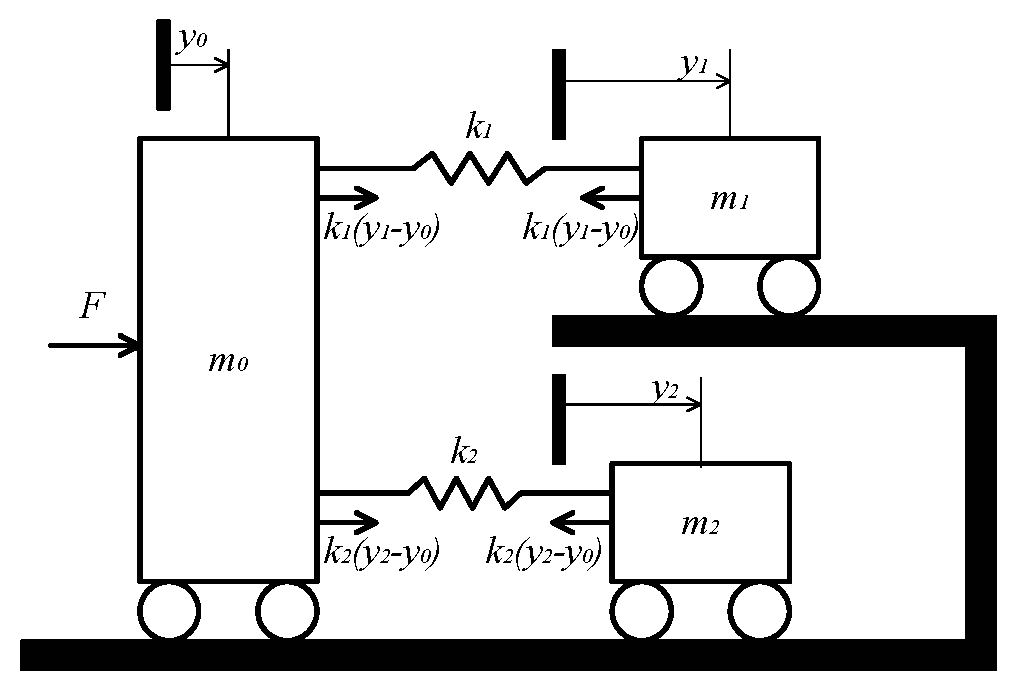
\includegraphics[width=0.7\linewidth]{sfigure/car3.eps}
  \caption{３質量系}
  \label{fig_3mass}
 \end{center}
\end{figure}

\setcounter{figure}{\value{countersave}} %%%%式カウンター復活

\end{frame}

%%%%%%%%%%%%%%%%%%%%%%%%%%%%%%%%%%%%%%%%%%%%%%%%%%%%%%%%%%%%%%
\begin{frame}[t]
\frametitle{1.5 可制御性 ＜演習＞ ３質量系の可制御性}
%-------------------------------------------------------------
Fig.\ref{fig_3mass}で用いた３質量系の状態方程式は
\small{
\begin{align}
 \frac{d}{dt} \left(\begin{array}{c}
           y_0 \\
         y_1 \\
         y_2 \\
         \frac{dy_0}{dt} \\
         \frac{dy_1}{dt} \\
         \frac{dy_2}{dt}
        \end{array}\right)
 &=
 \left(\begin{array}{cccccc}
        0 & 0 & 0 & 1 & 0 & 0      \\
        0 & 0 & 0 & 0 & 1 & 0      \\
        0 & 0 & 0 & 0 & 0 & 1      \\
  -\frac{k_1}{m_0} -\frac{k_2}{m_0}&  \frac{k_1}{m_0} &  \frac{k_2}{m_0} & 0 & 0 & 0 \\
   \frac{k_1}{m_1}                & -\frac{k_1}{m_1} &  0               & 0 & 0 & 0 \\
   \frac{k_2}{m_2}                &  0               & -\frac{k_2}{m_2} & 0 & 0 & 0
       \end{array}\right)
 \left(\begin{array}{c}
           y_0 \\
         y_1 \\
         y_2 \\
         \frac{dy_0}{dt} \\
         \frac{dy_1}{dt} \\
         \frac{dy_2}{dt}
       \end{array}\right)
 +
 \left(\begin{array}{c}
        0 \\
        0 \\
        0 \\
      \frac{1}{m_0} \\
      0 \\
      0
       \end{array}\right)
        F
\nonumber
\\
 \left(\begin{array}{c}
      y_0 \\
    y_1 \\
    y_2
       \end{array}\right)
 &=
 \left(\begin{array}{cccccc}
         1 & 0 & 0 & 0 & 0 & 0  \\
         0 & 1 & 0 & 0 & 0 & 0 \\
         0 & 0 & 1 & 0 & 0 & 0 \\
       \end{array}\right)
 \left(\begin{array}{c}
           y_0 \\
         y_1 \\
         y_2 \\
         \frac{dy_0}{dt} \\
         \frac{dy_1}{dt} \\
         \frac{dy_2}{dt}
       \end{array}\right)
\nonumber
\end{align}
}
となる．このシステムについて以下を確認せよ．

・$m_0=m_1=m_2=1$, $k_1=k_2=1$のとき，システムは不可制御

・$m_0=m_1=m_2=1$, $k_1=1$, $k_2=2$のとき，システムは可制御
\end{frame}


%%%%%%%%%%%%%%%%%%%%%%%%%%%%%%%%%%%%%%%%%%%%%%%%%%%%%%%%%%%%%%
\begin{frame}[t]
\frametitle{1.5 可制御性 ＜演習＞不可制御なシステムの分解}
%-------------------------------------------------------------
次のシステムが不可制御であることを確認し，可制御な部分と不可制御な部分に分けよ．\begin{align*}
  \frac{d}{dt}
  \left (
  \begin{array}{c}
   x_1 \\ x_2
  \end{array}
  \right )
  & =
  \left (
  \begin{array}{cc}
   0 & 1 \\
   -1 & 2
  \end{array}
  \right )
  \left (
  \begin{array}{c}
   x_1 \\ x_2
  \end{array}
  \right )
  +
  \left (
  \begin{array}{c}
   1 \\ 1
  \end{array}
  \right )
  u
\\
  y
  &=
  \left (
  \begin{array}{cc}
   1 & 1
  \end{array}
  \right )
  \left (
  \begin{array}{c}
   x_1 \\ x_2
  \end{array}
  \right )
\end{align*}
\end{frame}


%%%%%%%%%%%%%%%%%%%%%%%%%%%%%%%%%%%%%%%%%%%%%%%%%%%%%%%%%%%%%%
\begin{frame}[t]
\frametitle{1.6 可観測性 (定義)}
%-------------------------------------------------------------
状態方程式
\begin{align}
 \frac{dx}{dt} &= A x(t) + B u(t) \tag{\ref{state_eq}} \\
 y(t) &= C x(t) + D u(t) \tag{\ref{output_eq}}
\end{align}
\begin{block}{可観測}
システム(\ref{state_eq})(\ref{output_eq})において，有限時間$[0,t_1]$の入力$u(t),0 \leq t \leq t_1$と出力$y(t), 0 \leq t \leq t_1$から初期状態$x(0)=x_0$を一意に決定できるとき，システムは\Blue{\bf 可観測(observable)}であるという．
\end{block}

システムの\Blue{\bf 可観測性(observability)}は$C,A$行列のみで決定されるので，\Blue{\bf $(C,A)$可観測}と呼ばれることもある．

可観測とはシステムの入出力から状態が推定できるか否かという概念である．
\end{frame}


%%%%%%%%%%%%%%%%%%%%%%%%%%%%%%%%%%%%%%%%%%%%%%%%%%%%%%%%%%%%%%
\begin{frame}[t]
\frametitle{1.6 可観測性 (不可観測な状態方程式)}
%-------------------------------------------------------------
次のシステムを考える．
\begin{align}
 \frac{d}{dt}
  \left(\begin{array}{c}
         {x}_1 \\
   {x}_2
  \end{array}\right)
  &=
  \left(\begin{array}{cc}
         {A}_{11} & {A}_{12} \\
       {A}_{21} & {A}_{22}
  \end{array}\right)
  \left(\begin{array}{c}
         {x}_1 \\
   {x}_2
  \end{array}\right)
  +
  \left(\begin{array}{c}
         {B}_1 \\
   {B}_2
  \end{array}\right)
  u \\
 y &=
  \left(\begin{array}{cc}
         {C}_1 & C_2
  \end{array}\right)
  \left(\begin{array}{c}
         {x}_1 \\
   {x}_2
  \end{array}\right)
  + D u
\vspace{-5mm}
\end{align}
ここで
$x = \left(\begin{array}{c} {x}_1 \\ {x}_2 \end{array}\right) \in {\mathbb R}^n$,
$x_1 \in {\mathbb R}^r$, $x_2 \in {\mathbb R}^{n-r}$で，$A,B,C$行列は$x$の分割にあわせて定義されているものとする（例えば$A_{11} \in {\mathbb R}^{r \times r}$, $A_{12} \in {\mathbb R}^{r \times (n-r)}$など）．
このシステムを次のように書き下す．
\begin{align}
 \frac{dx_1}{dt} &= A_{11} x_1 + A_{12} x_2 + B_1 u
\label{eq:observable1} \\
 \frac{dx_2}{dt} &= A_{21} x_1 + A_{22} x_2 + B_2 u
\label{eq:observable2} \\
 y & = C_1 x_1 + C_2 x_2+ Du
\label{eq:observable03}
\end{align}
このシステムの状態$x_2$が出力$y$から見えない（観測できない）ためには$C_2=0$である必要がある．
\end{frame}


%%%%%%%%%%%%%%%%%%%%%%%%%%%%%%%%%%%%%%%%%%%%%%%%%%%%%%%%%%%%%%
\begin{frame}[t]
\frametitle{1.6 可観測性 (不可観測な状態方程式)}
%-------------------------------------------------------------
$C_2=0$とすると，状態方程式は以下となる．
\begin{align}
 \frac{d}{dt}
  \left(\begin{array}{c}
         {x}_1 \\
   {x}_2
  \end{array}\right)
  &=
  \left(\begin{array}{cc}
         {A}_{11} & {A}_{12} \\
       {A}_{21} & {A}_{22}
  \end{array}\right)
  \left(\begin{array}{c}
         {x}_1 \\
   {x}_2
  \end{array}\right)
  +
  \left(\begin{array}{c}
         {B}_1 \\
   {B}_2
  \end{array}\right)
  u \\
 y &=
  \left(\begin{array}{cc}
         {C}_1 & \Red{0}
  \end{array}\right)
  \left(\begin{array}{c}
         {x}_1 \\
   {x}_2
  \end{array}\right)
  + D u
\vspace{-5mm}
\end{align}
このシステムを書き下せば以下となる．
\begin{align}
 \frac{dx_1}{dt} &= A_{11} x_1 + A_{12} x_2 + B_1 u
\label{eq:observable1} \\
 \frac{dx_2}{dt} &= A_{21} x_1 + A_{22} x_2 + B_2 u
\label{eq:observable2} \\
 y & = C_1 x_1 + Du
\label{eq:observable3}
\end{align}
\end{frame}


%%%%%%%%%%%%%%%%%%%%%%%%%%%%%%%%%%%%%%%%%%%%%%%%%%%%%%%%%%%%%%
\begin{frame}[t]
\frametitle{1.6 可観測性 (不可観測な状態方程式)}
%-------------------------------------------------------------
\begin{align}
 \frac{dx_1}{dt} &= A_{11} x_1 + A_{12} x_2 + B_1 u
\tag{\ref{eq:observable1}} \\
 \frac{dx_2}{dt} &= A_{21} x_1 + A_{22} x_2 + B_2 u
\tag{\ref{eq:observable2}} \\
 y & = C_1 x_1 + Du
\tag{\ref{eq:observable3}}
\end{align}

(\ref{eq:observable3})より，出力$y$は$x_1$の影響を受ける．出力$y$は$x_2$の影響を直接は受けないが，(\ref{eq:observable1})より$x_1$が$x_2$の影響を受けるため，間接的に$x_2$も$y$に影響する可能性がある．

つまり，このシステムでは$x_1$も$x_2$も出力に影響を与える可能性がある．

言い換えれば出力$y$は$x_1,x_2$の両方の情報を持っているので，なんらか手法で出力$y$から状態$x = \left(\begin{array}{c} {x}_1 \\ {x}_2 \end{array}\right)$を決定できる可能性を持っている．
\end{frame}


%%%%%%%%%%%%%%%%%%%%%%%%%%%%%%%%%%%%%%%%%%%%%%%%%%%%%%%%%%%%%%
\begin{frame}[t]
\frametitle{1.6 可観測性 (不可観測な状態方程式)}
%-------------------------------------------------------------
しかし，もし，この状態方程式の$A_{12}$の部分が$0$行列であるとすれば
\begin{align}
 \frac{d}{dt}
  \left(\begin{array}{c}
         {x}_1 \\
   {x}_2
  \end{array}\right)
  &=
  \left(\begin{array}{cc}
         {A}_{11} & \Red{0} \\
       {A}_{21} & {A}_{22}
  \end{array}\right)
  \left(\begin{array}{c}
         {x}_1 \\
   {x}_2
  \end{array}\right)
  +
  \left(\begin{array}{c}
         {B}_1 \\
   {B}_2
  \end{array}\right)
  u
\label{eq:unobservable1} \\
 y &=
  \left(\begin{array}{cc}
         {C}_1 & 0
  \end{array}\right)
  \left(\begin{array}{c}
         {x}_1 \\
   {x}_2
  \end{array}\right)
  + D u
\label{eq:unobservable2}\vspace{-3mm}
\end{align}
であり，書き下すと\vspace{-3mm}
\begin{align}
 \frac{dx_1}{dt} &= A_{11} x_1 \ \ \ \ \ \ \ \ \ \ \ + B_1 u
\label{eq:unobservable3} \\
 \frac{dx_2}{dt} &= A_{21} x_1 + A_{22} x_2 + B_2 u
\label{eq:unobservable4} \\
 y & = C_1 x_1 + Du
\label{eq:unobservable5}\vspace{-3mm}
\end{align}
となり
\begin{itemize}
\item (\ref{eq:unobservable5})より出力$y$は$x_1$の影響を受けるが，$x_2$の影響は直接は受けない．
\item (\ref{eq:unobservable3})より$x_1$も$x_2$の影響を受けないため，出力$y$は$x_2$の影響をまったく受けない．
\end{itemize}
つまり，出力$y$は$x_2$の情報を持たないため，何をしても出力（と入力）から$x_2$を決定することができない．つまり不可観測なシステムであることがわかる．
\end{frame}



%%%%%%%%%%%%%%%%%%%%%%%%%%%%%%%%%%%%%%%%%%%%%%%%%%%%%%%%%%%%%%
\begin{frame}[t]
\frametitle{1.6 可観測性 (不可観測な状態方程式)}
%-------------------------------------------------------------
%\vspace{-5mm}

\begin{align}
  \begin{array}{cc}
    \left(
      \begin{array}{c}
         x_1 \\  x_2
      \end{array}
    \right)\in \mathbb{R}^{n} &
    \begin{aligned}
       x_1 \in& \mathbb{R}^r \\
       x_2 \in& \mathbb{R}^{n-r} \\
    \end{aligned}
  \end{array} \notag
\end{align}
\begin{align}
  \frac{d}{dt}
  \left(
    \begin{array}{c}
      x_1 \\ x_2
    \end{array}
  \right) =& \left(
    \begin{array}{cc}
      A_{11} & \textcolor{red}{0} \\ A_{21} & A_{22}
    \end{array}
  \right)
  \left(
    \begin{array}{c}
      x_1 \\ x_2
    \end{array}
  \right) +
  \left(
    \begin{array}{c}
      B_1 \\ B_2
    \end{array}
  \right) u \tag{\ref{eq:unobservable1}}\\
  y =& \left(
    \begin{array}{cc}
      C_1 & \textcolor{red}{0}
    \end{array}
  \right)
  \left(
    \begin{array}{c}
      x_1 \\ x_2
    \end{array}
  \right) + D u \tag{\ref{eq:unobservable2}}
\end{align}
\begin{itemize}
\item (\ref{eq:unobservable5})より出力$y$は$x_1$の影響を受けるが，$x_2$の影響は直接は受けない．
\item (\ref{eq:unobservable3})より$x_1$も$x_2$の影響を受けないため，出力$y$は$x_2$の影響をまったく受けない．
\end{itemize}
つまり，出力$y$は$x_2$の情報を持たないため，何をしても出力（と入力）から$x_2$を決定することができない．つまり不可観測なシステムであることがわかる．
\begin{quote}
(\ref{eq:unobservable1})(\ref{eq:unobservable2})で表されるシステムや，座標変換で(\ref{eq:unobservable1})(\ref{eq:unobservable2})に変換されるシステムは不可観測なシステムである．
\end{quote}
\addtocounter{figure}{+1}
\end{frame}


%%%%%%%%%%%%%%%%%%%%%%%%%%%%%%%%%%%%%%%%%%%%%%%%%%%%%%%%%%%%%%
\begin{frame}[t]
\frametitle{1.6 可観測性 (不可観測な状態方程式)}
%-------------------------------------------------------------

\ \vspace*{-1.1cm}

  \begin{align}
    \begin{array}{cc}
      \left(
        \begin{array}{c}
           x_1 \\  x_2
        \end{array}
      \right)\in \mathbb{R}^{n} &
      \begin{aligned}
         x_1 \in& \mathbb{R}^r \\
         x_2 \in& \mathbb{R}^{n-r} \\
      \end{aligned}
    \end{array} \notag
  \end{align}
  \begin{align}
    \frac{d}{dt}
    \left(
      \begin{array}{c}
        x_1 \\ x_2
      \end{array}
    \right) =& \left(
      \begin{array}{cc}
        A_{11} & \textcolor{red}{0} \\ A_{21} & A_{22}
      \end{array}
    \right)
    \left(
      \begin{array}{c}
        x_1 \\ x_2
      \end{array}
    \right) +
    \left(
      \begin{array}{c}
        B_1 \\ B_2
      \end{array}
    \right) u \tag{\ref{eq:unobservable1}}\\
    y =& \left(
      \begin{array}{cc}
        C_1 & \textcolor{red}{0}
      \end{array}
    \right)
    \left(
      \begin{array}{c}
        x_1 \\ x_2
      \end{array}
    \right) + D u \tag{\ref{eq:unobservable2}}
  \end{align}
  \begin{tikzpicture}[every node/.style={thick,circle,inner sep=0pt},overlay,blue]
    \only<2,3,4>{
      % \draw [help lines] (0,0) grid (10,4);%(0,0)から(10,4)までの"細線の方眼"
      \node[draw=blue, minimum size=0.5cm] (y) at (3.75,0.8)  {};
      \node[draw=blue, minimum size=0.5cm] (C1) at (4.8,0.8)  {};
      \node[minimum size=0.5cm] (C2) at (5.5,0.85)  {};
      \path[every node/.style={thick}]
       (y) edge[->, bend left=20] node {} (C1)
       (y) edge[->, bend left=40] node {} (C2);
    }
    \only<3,4>{
      \node[draw=blue, minimum size=0.5cm] (yx1) at (6.55,1.0)  {};
      \node[minimum size=0.5cm] (yx2) at (6.55,0.5)  {};
      \path[every node/.style={thick}]
       (C1) edge[->, bend left=20] node {} (yx1)
       (C2) edge[->, bend left=20, dashed] node {} (yx2);
    }
    \only<4>{
      \node[draw=blue, minimum size=0.5cm] (dx1) at (3.2,2.0)  {};
      \node[minimum size=0.5cm] (A12) at (5.95,2.0) {};
      \node[minimum size=0.5cm] (x2) at (7.3,1.6)  {};
      \path[every node/.style={thick}]
       (dx1) edge[->, bend left=20] node {} (A12)
       (A12) edge[->, bend left=15, dashed] node {} (x2);
    }
  \end{tikzpicture}
  \begin{align}
    \frac{dx_1}{dt} &= A_{11} x_1 \ \ \ \ \ \ \ \ \ \ \ + B_1 u
    \tag{\ref{eq:unobservable3}} \\
     \frac{dx_2}{dt} &= A_{21} x_1 + A_{22} x_2 + B_2 u
    \tag{\ref{eq:unobservable4}} \\
     y & = C_1 x_1 + Du
    \tag{\ref{eq:unobservable5}}
  \end{align}
  \begin{tikzpicture}[every node/.style={thick,circle,inner sep=0pt},overlay,blue]
    \only<5,6>{
      % \draw [help lines] (0,0) grid (10,4);%(0,0)から(10,4)までの"細線の方眼"
      \node[draw=blue, minimum size=0.5cm] (dx1) at (4.25,2.65)  {};
      \node[draw=blue, minimum size=0.5cm] (y) at (4.4,0.9) {};
      \node[draw=blue, minimum size=0.5cm] (yx1) at (5.5,0.9) {};
      \node[draw=blue, minimum size=0.5cm, dashed] (x2) at (6.6,2.4) {};
      \path[every node/.style={thick}]
        (dx1) edge[->, bend left=20] node {$x_2$} (x2)
        (y) edge[->, bend left=40] node {} (yx1);
    }
    \only<6>{
      \node[draw=blue, rectangle, minimum width=1.5cm, minimum height=0.6cm, rounded corners]
       (unCtrl) at (9.1 ,0.7) {不可観測};
      \node[draw=blue, rectangle, minimum width=3.0cm, minimum height=0.8cm, rounded corners]
       (rect) at (5.5 ,0.9) {};
      \path[every node/.style={thick}]
      (unCtrl) edge[->, bend left=20] node {} (rect);
    }
  \end{tikzpicture}
\vspace*{-0.3cm}

  %%%%%%%%%%%%%%%%%%%%%%%%%%%%%%%% 説明文 %%%%%%%%%%%%%%%%%%%%%%%%%%%%%%%%%%%%%%%
  \only<1>{
    可制御性は$A, C$ 行列のみに依存する．出力$y$ への影響を考察する．
  }
  \only<2>{
    出力$y$ は$C$ 行列を通して影響を受ける．
  }
  \only<3>{
    出力$y$は$x_1$の影響を受けるが，$x_2$の影響は直接は受けない．
  }
  \only<4>{
    $x_1$も$x_2$の影響を受けないため，最終的に出力$y$は$x_2$の影響をまったく受けなくなってしまう．
  }
  \end{frame}


%%%%%%%%%%%%%%%%%%%%%%%%%%%%%%%%%%%%%%%%%%%%%%%%%%%%%%%%%%%%%%
\begin{frame}[t]
\frametitle{1.6 可観測性 (可観測性の条件)}
%-------------------------------------------------------------
不可観測なシステム
\begin{align}
  \begin{array}{cc}
    \left(
      \begin{array}{c}
         x_1 \\  x_2
      \end{array}
    \right)\in \mathbb{R}^{n} &
    \begin{aligned}
       x_1 \in& \mathbb{R}^r \\
       x_2 \in& \mathbb{R}^{n-r} \\
    \end{aligned}
  \end{array} \notag
\end{align}
\begin{align}
  \frac{d}{dt}
  \left(
    \begin{array}{c}
      x_1 \\ x_2
    \end{array}
  \right) =& \left(
    \begin{array}{cc}
      A_{11} & \textcolor{red}{0} \\ A_{21} & A_{22}
    \end{array}
  \right)
  \left(
    \begin{array}{c}
      x_1 \\ x_2
    \end{array}
  \right) +
  \left(
    \begin{array}{c}
      B_1 \\ B_2
    \end{array}
  \right) u \tag{\ref{eq:unobservable1}}\\
  y =& \left(
    \begin{array}{cc}
      C_1 & \textcolor{red}{0}
    \end{array}
  \right)
  \left(
    \begin{array}{c}
      x_1 \\ x_2
    \end{array}
  \right) + D u \tag{\ref{eq:unobservable2}}
\end{align}
(\ref{eq:unobservable1})(\ref{eq:unobservable2})について
\begin{equation}
 N^T =
  \left(\begin{array}{c}
         C        \\
   C A      \\
   C A^2    \\
   \vdots   \\
   C A^{n-1}
  \end{array}\right)
\end{equation}
を計算してみよう．
\end{frame}


%%%%%%%%%%%%%%%%%%%%%%%%%%%%%%%%%%%%%%%%%%%%%%%%%%%%%%%%%%%%%%
\begin{frame}[t]
\frametitle{1.6 可観測性 (可観測性の条件)}
%-------------------------------------------------------------
\begin{equation}
 N^T =
  \left(\begin{array}{c}
         C        \\
   C A      \\
   C A^2    \\
   \vdots   \\
   C A^{n-1}
  \end{array}\right)
 =
  \left(\begin{array}{lr}
       (C_1           & 0) \\
     (C_1 A_{11}       & 0) \\
     (C_1 A_{11}^2     & 0) \\
     \vdots   \\
     (C_1 A_{11}^{n-1} & 0)
  \end{array}\right)
\end{equation}
となる．$x \in {\mathbb R}^n$, $ y \in {\mathbb R}^p $より$A\in {\mathbb R}^{n \times n}$, $C \in {\mathbb R}^{p \times n}$であるから$N^T \in {\mathbb R}^{np \times n}$であるが，$x_2$にあたる右側の$n-r$列が$0$である．これは
\begin{align}
 \mbox{rank}\ N^T
 &= \mbox{rank}
  \left(\begin{array}{c}
         C        \\
   C A      \\
   C A^2    \\
   \vdots   \\
   C A^{n-1}
  \end{array}\right)
   \leq r < n
\end{align}
であることを示している．
\end{frame}


%%%%%%%%%%%%%%%%%%%%%%%%%%%%%%%%%%%%%%%%%%%%%%%%%%%%%%%%%%%%%%
\begin{frame}[t]
\frametitle{1.6 可観測性 (可観測性の条件)}
%-------------------------------------------------------------
不可観測なシステム(\ref{eq:unobservable1})(\ref{eq:unobservable2})を$\bar{A}= T^{-1} A T$, $\bar{C} = C T$と座標変換したシステムについても同様に$\bar{N}^T$を計算してみると
\begin{align}
 \bar{N}^T
 &=
  \left(\begin{array}{c}
     \bar{C}        \\
   \bar{C} \bar{A}      \\
   \bar{C} \bar{A}^2    \\
   \vdots   \\
   \bar{C} \bar{A}^{n-1}
  \end{array}\right)
 =
  \left(\begin{array}{c}
     CT        \\
   CT T^{-1}AT      \\
   CT T^{-1}A^2T    \\
   \vdots   \\
   CT T^{-1}A^{n-1}T
  \end{array}\right)
 =
  \left(\begin{array}{c}
     C T       \\
   C A T     \\
   C A^2 T   \\
   \vdots   \\
   C A^{n-1}T
  \end{array}\right)
 =
  \left(\begin{array}{c}
         C        \\
   C A      \\
   C A^2    \\
   \vdots   \\
   C A^{n-1}
  \end{array}\right)
  T
\nonumber \\
 &= N^T T
\end{align}
となり，$T$が正則であることから
\begin{align}
 \mbox{rank}\ \bar{N^T} & = \mbox{rank}\ {N^T} \leq r < n
\end{align}
となる．
\end{frame}


%%%%%%%%%%%%%%%%%%%%%%%%%%%%%%%%%%%%%%%%%%%%%%%%%%%%%%%%%%%%%%
\begin{frame}[t]
\frametitle{1.6 可観測性 (可観測性の条件)}
%-------------------------------------------------------------
\begin{block}{}
不可観測なシステム
に座標変換で変換できるシステムは次式が成り立つ．\\
   $$\mbox{rank}\ N^T
   = \mbox{rank}
    \left(\begin{array}{c}
           C        \\
     C A      \\
     C A^2    \\
     \vdots   \\
     C A^{n-1}
    \end{array}\right)
    < n$$
\end{block}
逆に次のことが分かっている．
\begin{block}{}
   $$\mbox{rank}\ N^T
   = \mbox{rank}
    \left(\begin{array}{c}
           C        \\
     C A      \\
     C A^2    \\
     \vdots   \\
     C A^{n-1}
    \end{array}\right)
    < n$$
    を満たすシステムは不可観測なシステム
    に座標変換で変換できる．
\end{block}
\end{frame}


%%%%%%%%%%%%%%%%%%%%%%%%%%%%%%%%%%%%%%%%%%%%%%%%%%%%%%%%%%%%%%
\begin{frame}[t]
\frametitle{1.6 可観測性 (可観測性の条件)}
%-------------------------------------------------------------
つまり，
\begin{block}{}
システムが不可観測なシステム(\ref{eq:unobservable1})(\ref{eq:unobservable2})に座標変換で変換できるための必要十分条件は
   $$\mbox{rank}\ N^T
   = \mbox{rank}
    \left(\begin{array}{c}
           C        \\
     C A      \\
     C A^2    \\
     \vdots   \\
     C A^{n-1}
    \end{array}\right)
    < n$$
\end{block}
となる．これは不可観測なシステムに対する考察である．
\end{frame}


%%%%%%%%%%%%%%%%%%%%%%%%%%%%%%%%%%%%%%%%%%%%%%%%%%%%%%%%%%%%%%
\begin{frame}[t]
\frametitle{1.6 可観測性 (可観測性の条件)}
%-------------------------------------------------------------
可観測に関してはつぎが成り立つことがわかっている．
\begin{block}{可観測性の条件}
システムが可観測であるための必要十分条件は
  $$\mbox{rank}\ N^T
  = \mbox{rank}
    \left(\begin{array}{c}
           C        \\
     C A      \\
     C A^2    \\
     \vdots   \\
     C A^{n-1}
    \end{array}\right)
  = n$$
\end{block}
このように$N$は可観測性を判断するために重要な役割を果たすので，$N$は\Blue{\bf 可観測性行列(observability matrix)}と呼ばれている.
\end{frame}


%%%%%%%%%%%%%%%%%%%%%%%%%%%%%%%%%%%%%%%%%%%%%%%%%%%%%%%%%%%%%%
\begin{frame}[t]
\frametitle{1.6 可観測性 (不可観測性なシステムの分解)}
%-------------------------------------------------------------
システムが可観測でないとき，つまり
\begin{equation}
 \rank N^T = r < n
\end{equation}
のときを考える．このとき$N^T$の行ベクトルの中から線形独立なもの$r$本を選
びこれを$w_1^T, w_2^T, \cdots, w_r^T$と定義する．また$n-r$本の行ベ
クトル$w_{r+1}^T, w_{r+2}^T, \cdots, w_n^T$を
\begin{equation}
 W = \left(\begin{array}{c}
            w_1^T \\
      w_2^T \\
      \vdots \\
      w_r^T \\
      w_{r+1}^T \\
      \vdots \\
      w_n^T
     \end{array}\right)
\end{equation}
が正則になるように選ぶ．
\end{frame}


%%%%%%%%%%%%%%%%%%%%%%%%%%%%%%%%%%%%%%%%%%%%%%%%%%%%%%%%%%%%%%
\begin{frame}[t]
\frametitle{1.6 可観測性 (不可観測性なシステムの分解)}
%-------------------------------------------------------------
さらに$T=W^{-1}$とすると簡単な代数計算によりこの
行列$T$により座標変換されたシステムが
\begin{align}
 \frac{d}{dt}
  \left(\begin{array}{c}
         \bar{x}_1 \\
   \bar{x}_2
  \end{array}\right)
  &=
  \left(\begin{array}{cc}
         \bar{A}_{11} & 0 \\
   \bar{A}_{21} & \bar{A}_{22}
  \end{array}\right)
  \left(\begin{array}{c}
         \bar{x}_1 \\
   \bar{x}_2
  \end{array}\right)
  +
  \left(\begin{array}{c}
         \bar{B}_1 \\
   \bar{B}_2
  \end{array}\right)
  u \\
 y &=
  \left(\begin{array}{cc}
         \bar{C}_1 & 0
  \end{array}\right)
  \left(\begin{array}{c}
         \bar{x}_1 \\
   \bar{x}_2
  \end{array}\right)
  + D u
\end{align}
と表わされることが分かる．
\end{frame}


%%%%%%%%%%%%%%%%%%%%%%%%%%%%%%%%%%%%%%%%%%%%%%%%%%%%%%%%%%%%%%
\begin{frame}[t]
\frametitle{1.6 可観測性 (不可観測性なシステムの分解)}
%-------------------------------------------------------------
例)可制御性の例と同じ以下のようなシステムを考える．
\begin{align}
 \frac{d}{dt}
  \left(
   \begin{array}{c}
    x_1 \\
    x_2
   \end{array}
  \right) &=
  \left(
   \begin{array}{cc}
    1 & 0 \\
    0 & 1
   \end{array}
  \right)
  \left(
   \begin{array}{c}
    x_1 \\
    x_2
   \end{array}
  \right) +
  \left(
   \begin{array}{c}
    1 \\
    1
   \end{array}
  \right) u \\
 y &=
  \left(
   \begin{array}{cc}
    1 & 1
   \end{array}
  \right)
  \left(
   \begin{array}{c}
    x_1 \\
    x_2
   \end{array}
  \right)
\end{align}
このとき，可観測性行列$N$は
\begin{equation}
 N^T =
  \left(
   \begin{array}{c}
    C \\
    CA
   \end{array}
  \right) =
  \left(
   \begin{array}{cc}
    1 & 1 \\
    1 & 1
   \end{array}
  \right)
\end{equation}
となり，明らかに$\rank N = 1$であるので，このシステムは可観測ではない．
ここで，$w_1^T = (\begin{array}{cc}1 & 1\end{array})$,
$w_2^T = (\begin{array}{cc}0 & 1\end{array})$と選ぶことで，
\begin{equation}
 \begin{array}{cc}
  W =
   \left(
    \begin{array}{cc}
     1 & 1 \\
     0 & 1
    \end{array}
   \right),
   &
  W^{-1} =
   \left(
    \begin{array}{cc}
     1 & -1 \\
     0 & 1
    \end{array}
   \right)
 \end{array}
\end{equation}
のように正則な行列$W$を選ぶことができる．
\end{frame}


%%%%%%%%%%%%%%%%%%%%%%%%%%%%%%%%%%%%%%%%%%%%%%%%%%%%%%%%%%%%%%
\begin{frame}[t]
\frametitle{1.6 可観測性 (不可観測性なシステムの分解)}
%-------------------------------------------------------------
この$W^{-1} = T$により座標変換を行うと，
\begin{align}
 \bar{A} &= T^{-1}AT =
 \left(
 \begin{array}{cc}
  1 & 1 \\
  0 & 1
 \end{array}
 \right)
 \left(
 \begin{array}{cc}
  1 & 0 \\
  0 & 1
 \end{array}
 \right)
 \left(
 \begin{array}{cc}
  1 & -1 \\
  0 & 1
 \end{array}
 \right) =
 \left(
 \begin{array}{cc}
  1 & 0 \\
  0 & 1
 \end{array}
 \right) \\
 \bar{B} &= T^{-1}B =
 \left(
 \begin{array}{cc}
  1 & 1 \\
  0 & 1
 \end{array}
 \right)
 \left(
 \begin{array}{c}
  1 \\
  1
 \end{array}
 \right) =
 \left(
 \begin{array}{c}
  2 \\
  1
 \end{array}
 \right) \\
 \bar{C} &= CT =
 \left(
 \begin{array}{cc}
  1 & 1
 \end{array}
 \right)
 \left(
 \begin{array}{cc}
  1 & -1 \\
  0 & 1
 \end{array}
 \right) =
 \left(
 \begin{array}{cc}
  1 & 0
 \end{array}
 \right)
\end{align}
となるので，座標変換後のシステム
\begin{align}
 \frac{d}{dt}
  \left(
   \begin{array}{c}
    \bar{x}_1 \\
    \bar{x}_2
   \end{array}
  \right) &=
  \left(
   \begin{array}{cc}
    1 & \Red{0} \\
    0 & 1
   \end{array}
  \right)
  \left(
   \begin{array}{c}
    \bar{x}_1 \\
    \bar{x}_2
   \end{array}
  \right) +
  \left(
   \begin{array}{c}
    2 \\
    1
   \end{array}
  \right) u \\
 y &=
  \left(
   \begin{array}{cc}
    1 & \Red{0}
   \end{array}
  \right)
  \left(
   \begin{array}{c}
    \bar{x}_1 \\
    \bar{x}_2
   \end{array}
  \right)
\end{align}
では確かに出力$y$は状態$\bar{x}_2$の影響を受けていない．
\end{frame}

%%%%%%%%%%%%%%%%%%%%%%%%%%%%%%%%%%%%%%%%%%%%%%%%%%%%%%%%%%%%%%
\begin{frame}[t]
\frametitle{1.6 可観測性 ＜演習＞３質量系の可観測性}
%-------------------------------------------------------------
\setcounter{countersave}{\value{figure}} %%%%式カウンターsave
\setcounter{figure}{\value{fig:three-mass}}

\begin{figure}[htbp]
 \begin{center}
  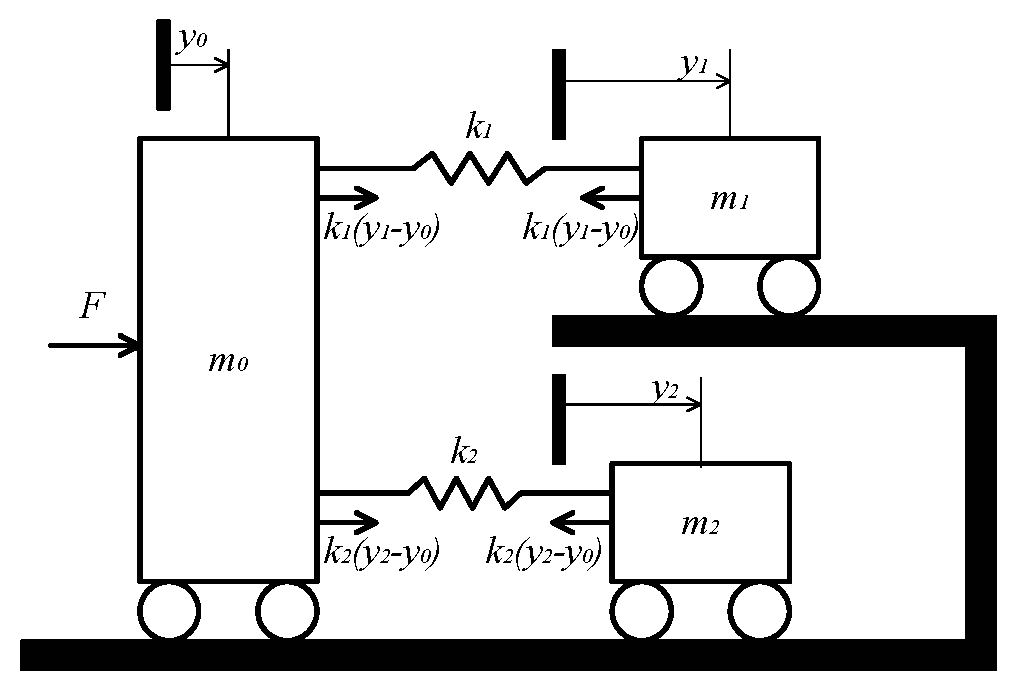
\includegraphics[width=0.7\linewidth]{sfigure/car3.eps}
  \caption{３質量系}
  \label{fig_3mass}
 \end{center}
\end{figure}

\setcounter{figure}{\value{countersave}} %%%%式カウンター復活

\end{frame}

%%%%%%%%%%%%%%%%%%%%%%%%%%%%%%%%%%%%%%%%%%%%%%%%%%%%%%%%%%%%%%
\begin{frame}[t]
\frametitle{1.6 可観測性 ＜演習＞３質量系の可観測性}
%-------------------------------------------------------------
Fig.\ref{fig_3mass}の３質量系で，出力が$y=y_0$の場合，状態方程式と出力方程式は
\small{
\begin{align}
 \frac{d}{dt} \left(\begin{array}{c}
           y_0 \\
         y_1 \\
         y_2 \\
         \frac{dy_0}{dt} \\
         \frac{dy_1}{dt} \\
         \frac{dy_2}{dt}
        \end{array}\right)
 &=
 \left(\begin{array}{cccccc}
        0 & 0 & 0 & 1 & 0 & 0      \\
        0 & 0 & 0 & 0 & 1 & 0      \\
        0 & 0 & 0 & 0 & 0 & 1      \\
  -\frac{k_1}{m_0} -\frac{k_2}{m_0}&  \frac{k_1}{m_0} &  \frac{k_2}{m_0} & 0 & 0 & 0 \\
   \frac{k_1}{m_1}                & -\frac{k_1}{m_1} &  0               & 0 & 0 & 0 \\
   \frac{k_2}{m_2}                &  0               & -\frac{k_2}{m_2} & 0 & 0 & 0
       \end{array}\right)
 \left(\begin{array}{c}
           y_0 \\
         y_1 \\
         y_2 \\
         \frac{dy_0}{dt} \\
         \frac{dy_1}{dt} \\
         \frac{dy_2}{dt}
       \end{array}\right)
 +
 \left(\begin{array}{c}
        0 \\
        0 \\
        0 \\
      \frac{1}{m_0} \\
      0 \\
      0
       \end{array}\right)
        F
\nonumber
\\
y &=
 \left(\begin{array}{cccccc}
         1 & 0 & 0 & 0 & 0 & 0
       \end{array}\right)
 \left(\begin{array}{c}
           y_0 \\
         y_1 \\
         y_2 \\
         \frac{dy_0}{dt} \\
         \frac{dy_1}{dt} \\
         \frac{dy_2}{dt}
       \end{array}\right)
\nonumber
\end{align}
}
となる．このシステムについて以下を確認せよ．

・$m_0=m_1=m_2=1$, $k_1=k_2=1$のとき，システムは不可観測

・$m_0=m_1=m_2=1$, $k_1=1$, $k_2=2$のとき，システムは可観測
\end{frame}


%%%%%%%%%%%%%%%%%%%%%%%%%%%%%%%%%%%%%%%%%%%%%%%%%%%%%%%%%%%%%%
\begin{frame}[t]
\frametitle{1.7 システムの応答 (遷移行列)}
%-------------------------------------------------------------
指数関数のテーラー展開が
\begin{equation}
  e^{a} = 1 + a + \frac{1}{2!} a^2
        + \frac{1}{3!} a^3  + \cdots
\end{equation}
と表されることを利用して行列の指数関数を次式で定義する．
\begin{equation}
 e^{At} = I + At + \frac{1}{2!} A^2 t^2
        + \frac{1}{3!} A^3 t^3 + \cdots
\end{equation}
$e^{At}$は\Blue{\bf {遷移行列}(transition matrix)}と呼ばれている．
\end{frame}


%%%%%%%%%%%%%%%%%%%%%%%%%%%%%%%%%%%%%%%%%%%%%%%%%%%%%%%%%%%%%%
\begin{frame}[t]
\frametitle{1.7 システムの応答 ($u=0$の場合の状態方程式の解)}
%-------------------------------------------------------------
状態方程式
\begin{align}
   \frac{dx}{dt} &= A x(t) + B u(t) \tag{\ref{state_eq}} \\
   y(t) &= C x(t) + D u(t) \tag{\ref{output_eq}}
\end{align}
状態方程式(\ref{state_eq})において$u(t) = 0$としたとき次式となる．
\begin{align}
\frac{dx}{dt} = Ax(t) \label{autonomous}
\end{align}
この解$x(t)$は$x(0)=x_0$として遷移行列を用いて次のように表わされる．
\begin{align}
 x(t) = e^{At} x_0 \label{eat}
\end{align}
\end{frame}


%%%%%%%%%%%%%%%%%%%%%%%%%%%%%%%%%%%%%%%%%%%%%%%%%%%%%%%%%%%%%%
\begin{frame}[t]
\frametitle{1.7 システムの応答 ($u=0$の場合の状態方程式の解)}
%-------------------------------------------------------------
\vspace*{-0.7cm}

\begin{align}
\frac{dx}{dt} = Ax(t) \tag{\ref{autonomous}}
\end{align}
\vspace*{-1.2cm}

\begin{align}
 x(t) = e^{At} x_0 \tag{\ref{eat}}
\end{align}

(\ref{eat})で表される$x(t)$の微分を計算することにより，(\ref{autonomous})が満たされることが証明できる．
\vspace{0cm}
\begin{align}
 \frac{d}{dt}x(t)
 &= \frac{d}{dt}e^{At} x_0 \\
 &= \frac{d}{dt}
 \left(I + At + \frac{1}{2!} A^2 t^2 + \frac{1}{3!} A^3 t^3 +
 \frac{1}{4!} A^4 t^4 + \cdots\right)x_0 \nonumber \\
 &= \left(0 + A + \frac{2}{2!} A^2 t + \frac{3}{3!} A^3 t^2 +
 \cdots\right)x_0 \nonumber \\
 &= A
 \left(I + At + \frac{1}{2!} A^2 t^2 + \frac{1}{3!} A^3 t^3 + \cdots
 \right)x_0 \nonumber \\
 &= A e^{At} x_0 \nonumber \\
 &= Ax(t)
\end{align}
\end{frame}


%%%%%%%%%%%%%%%%%%%%%%%%%%%%%%%%%%%%%%%%%%%%%%%%%%%%%%%%%%%%%%
\begin{frame}[t]
\frametitle{1.7 システムの応答 (遷移行列の性質)}
%-------------------------------------------------------------
遷移行列と呼ばれる$e^{At}$には以下のような性質がある．
\begin{align}
 \frac{d}{dt} e^{At} &= A e^{At}
          \hspace{1.0cm}
          \because \mbox{すでに示した．}\\
 e^{A 0}          &= I
           \hspace{1.6cm}
           \because x(0) = e^{A0}x(0) = I x(0) \\
 e^{A(t_1 + t_2)} &= e^{At_1} e^{A t_2}
           \hspace{0.5cm}
           \because x(t_1+t_2) = e^{At_1}x(t_2) = e^{At_1} e^{At_2} x(0)
                  = e^{A(t_1+t_2)}x(0)\\
 \left \{ e^{At} \right \}^{-1} & = e^{-At}
          \hspace{1.1cm}
          \because I = e^{A0} = e^{A(t-t)} = e^{At}e^{-At}\\
 e^{At}           &= T e^{T^{-1}AT t} T^{-1}
 \label{e_cor}
\end{align}
\end{frame}

%%%%%%%%%%%%%%%%%%%%%%%%%%%%%%%%%%%%%%%%%%%%%%%%%%%%%%%%%%%%%%
\begin{frame}[t]
\frametitle{1.7 システムの応答 (遷移行列の性質)}
%-------------------------------------------------------------
最後の性質は以下のように証明される．
\begin{align}
 Te^{T^{-1}ATt}T^{-1}
 &= T\left\{
 I + (T^{-1}AT)t + \frac{1}{2!}(T^{-1}AT)^2t^2 +
 \frac{1}{3!}(T^{-1}AT)^3t^3 \cdots \right\}T^{-1}
\nonumber \\
 &= T\left\{
 I + (T^{-1}AT)t + \frac{1}{2!}(T^{-1}A^2T)t^2 +
 \frac{1}{3!}(T^{-1}A^3T)t^3 \cdots \right\}T^{-1}
\nonumber \\
 &= T\left\{
 T^{-1}\left(I + At + \frac{1}{2!}A^2t^2 +
 \frac{1}{3!}A^3t^3 + \cdots\right)T \right\}T^{-1}
\nonumber \\
 &= e^{At}
\\
 & \hspace{0cm}
 \because
 (T^{-1}AT)^i = T^{-1}ATT^{-1}AT\cdots T^{-1}ATT^{-1}AT = T^{-1}A^iT
\end{align}
\end{frame}


%%%%%%%%%%%%%%%%%%%%%%%%%%%%%%%%%%%%%%%%%%%%%%%%%%%%%%%%%%%%%%
\begin{frame}[t]
\frametitle{1.7 システムの応答 (遷移行列の性質)}
%-------------------------------------------------------------
もし$A$が\Blue{\bf {対角行列}(diagonal matrix)}$\Lambda$
\begin{equation}
 \Lambda =
  \left(\begin{array}{cccc}
         \lambda_1 & 0         & \cdots & 0 \\
   0         & \lambda_2 &        & 0 \\
   \vdots    &           & \ddots & \\
   0         & 0         &        & \lambda_n
  \end{array}\right)
\end{equation}
であるならば
\end{frame}


%%%%%%%%%%%%%%%%%%%%%%%%%%%%%%%%%%%%%%%%%%%%%%%%%%%%%%%%%%%%%%
\begin{frame}[t]
\frametitle{1.7 システムの応答 (遷移行列の性質)}
%-------------------------------------------------------------
\vspace*{-0.7cm}

{\small
\begin{align}
 e^{\Lambda t}
 &= I + \Lambda t + \frac{1}{2!}\Lambda^2t^2 + \cdots \nonumber\\
 &=
 \left(\begin{array}{cccc}
        1      & 0 & \cdots & 0 \\
  0      & 1 &        & 0 \\
  \vdots &   & \ddots &   \\
  0      & 0 &        & 1
       \end{array}\right) +
 \left(\begin{array}{cccc}
        \lambda_1 & 0         & \cdots & 0 \\
  0         & \lambda_2 &        & 0 \\
  \vdots    &           & \ddots &   \\
  0         & 0         &        & \lambda_n
       \end{array}\right) t +
 \frac{1}{2!}
 \left(\begin{array}{cccc}
        \lambda_1^2 & 0         & \cdots & 0 \\
  0         & \lambda_2^2 &        & 0 \\
  \vdots    &           & \ddots &   \\
  0         & 0         &        & \lambda_n^2
       \end{array}\right) t^2 + \cdots \nonumber\\
 &=
 \left(\begin{array}{cccc}
        1 + \lambda_1 t + \frac{1}{2} \lambda_1^2 t^2 + \cdots & 0 & \cdots & 0 \\
  0      & 1 + \lambda_2 t + \frac{1}{2} \lambda_2^2 t^2 + \cdots &        & 0 \\
  \vdots &   & \ddots &   \\
  0      & 0 &        & 1 + \lambda_n t + \frac{1}{2} \lambda_n^2 t^2 + \cdots
       \end{array}\right)
\nonumber\\
 &=
 \left(\begin{array}{cccc}
        e^{\lambda_1 t} & 0               & \cdots & 0 \\
  0               & e^{\lambda_2 t} &        & 0 \\
  \vdots          &                 & \ddots & \\
  0               & 0               &        & e^{\lambda_n t}
       \end{array}\right)
 \label{e_diag}
\end{align}
}
となる．
\end{frame}


%%%%%%%%%%%%%%%%%%%%%%%%%%%%%%%%%%%%%%%%%%%%%%%%%%%%%%%%%%%%%%
\begin{frame}[t]
\frametitle{1.7 システムの応答 (入力を持つ状態方程式の解)}
%-------------------------------------------------------------
入力を持つ状態方程式(\ref{state_eq})の解は次で与えられる．
\begin{align}
  x(t) = e^{At} x_0 + \int_0^t e^{A(t-\tau)} B u (\tau) d \tau
  \label{response_w_input}
\end{align}
(証明)
\begin{align}
  \frac{dx}{dt}
  &=\frac{d}{dt} \left\{ e^{At} x_0 + \int_0^t e^{A(t-\tau)} B u (\tau) d \tau \right\}
\nonumber \\
  &=\frac{d}{dt} \left\{ e^{At} x_0 \right\}
    +\frac{d}{dt} \left\{ \int_0^t e^{A(t-\tau)} B u (\tau) d \tau \right\}
\nonumber\\
  &= A e^{At} x_0 + \frac {d}{dt} \left\{ e^{At} \int_0^t e^{A(-\tau)} B u (\tau) d \tau \right\}
\nonumber\\
  &= A e^{At} x_0 +  A e^{At} \int_0^t e^{A(-\tau)} B u (\tau) d \tau
        + e^{At}  e^{A(-t)} B u (t)\notag
\end{align}
\end{frame}


%%%%%%%%%%%%%%%%%%%%%%%%%%%%%%%%%%%%%%%%%%%%%%%%%%%%%%%%%%%%%%
\begin{frame}[t]
\frametitle{1.7 システムの応答 (入力を持つ状態方程式の解)}
%-------------------------------------------------------------
\vspace*{-5mm}

\begin{align}
  &= A e^{At} x_0 +  A e^{At} \int_0^t e^{A(-\tau)} B u (\tau) d \tau
        + e^{At}  e^{A(-t)} B u (t)
\nonumber\\
  &= A \left\{ e^{At} x_0 +  e^{At} \int_0^t e^{A(-\tau)} B u (\tau) d \tau \right\}
        +  B u (t)
\nonumber \\
  &= A \left\{ e^{At} x_0 +  \int_0^t e^{A(t-\tau)} B u (\tau) d \tau \right\}
        +  B u (t)
\nonumber\\
  & = Ax + Bu
\end{align}

これを用いれば出力$y$は以下で与えられる．
\begin{align}
  &y = Cx + Du \notag \\
  \Rightarrow \ \ \ \ \ &y(t)= Cx(t)+Du = Ce^{At} x_0 + C\int_0^t e^{A(t-\tau)} B u (\tau) d \tau + Du
\label{eq:outputresponse}
\end{align}
\end{frame}


%%%%%%%%%%%%%%%%%%%%%%%%%%%%%%%%%%%%%%%%%%%%%%%%%%%%%%%%%%%%%%
\begin{frame}[t]
\frametitle{1.8 システムの安定性 \\
(行列論：復習）固有値と固有ベクトル}
%-------------------------------------------------------------
$A v = \lambda v$
が成り立つベクトル$v (\neq 0)$が存在するとき，\\
\Blue{$\lambda$} $\in {\mathbb C}$(複素数) : Aの\Blue{\bf {固有値}(eigen value)}\\
\Blue{$v$} $\in {\mathbb C}^n$
 : $\lambda$に対する\Blue{\bf {固有ベクトル}(eigen vector)}

固有値$\lambda$は，
\[
 \begin{array}{rcl}
  \left\{A v = \lambda v, \quad v \neq 0\right\}
   &\Leftrightarrow& \left\{\lambda v - Av = 0, \quad v \neq 0\right\} \\
   &\Leftrightarrow& \left\{(\lambda I - A)v = 0, \quad v \neq 0\right\} \\
  &\Leftrightarrow& \lambda I - A \text{が逆行列を持たない} \\
  &\Leftrightarrow& \det(\lambda I - A) = 0
 \end{array}
\]
より，
\Blue{\bf {特性多項式} (characteristic polynomial)}
\begin{equation}
  \det(\lambda I - A) = 0
\end{equation}
を解くことで求められる．

特性方程式は$\lambda$ に対する$n$次の多項式となる．
つまり，固有値は$n$個ある．
\end{frame}


%%%%%%%%%%%%%%%%%%%%%%%%%%%%%%%%%%%%%%%%%%%%%%%%%%%%%%%%%%%%%%
\begin{frame}[t]
\frametitle{1.8 システムの安定性 \\
 (行列論：復習）固有値と固有ベクトル}
%-------------------------------------------------------------
例)
\begin{equation}
 A = \left(
      \begin{array}{cc}
       1 & 1 \\
       0 & 2 \\
      \end{array}
     \right)
\end{equation}
の\Blue{固有値は}，
$\det(\lambda I - A) = 0$を満たす$\lambda$，すなわち
\begin{equation}
 \det(\lambda I - A) =
 \det
 \left(
 \begin{array}{cc}
  \lambda - 1 & -1 \\
  0           & \lambda - 2 \\
 \end{array}
 \right) =
 (\lambda - 1)(\lambda - 2)
\end{equation}
より，\Blue{$\lambda = 1$ または $2$}である．

$\lambda = 1$のとき，
\begin{equation}
 \begin{array}{ccc}
 (\lambda I - A) v = 0
 &\Leftrightarrow&
 \left(
 \begin{array}{cc}
  0 & -1 \\
  0 & -1 \\
 \end{array}
 \right) v = 0
 \end{array}
\end{equation}
であるから，\Blue{$\lambda = 1$に対する固有ベクトルは
$v = (\begin{array}{cc}1 & 0\end{array})^T$}．

$\lambda = 2$のとき，
\begin{equation}
 \begin{array}{ccc}
 (\lambda I - A) v = 0
 &\Leftrightarrow&
 \left(
 \begin{array}{cc}
  1 & -1 \\
  0 & 0 \\
 \end{array}
 \right) v = 0
 \end{array}
\end{equation}
であるから，\Blue{$\lambda = 2$に対する固有ベクトルは
    $v = (\begin{array}{cc}1 & 1\end{array})^T$}．
\end{frame}


%%%%%%%%%%%%%%%%%%%%%%%%%%%%%%%%%%%%%%%%%%%%%%%%%%%%%%%%%%%%%%
\begin{frame}[t]
\frametitle{1.8 システムの安定性 \\
(行列論：復習) 行列の対角化}
%-------------------------------------------------------------
行列$A \in {\mathbb R}^{n \times n}$の固有値$\lambda_1, \lambda_2,
\cdots, \lambda_n$が相異なる場合，\\
すなわち$A v_i = \lambda_i v_i, (i = 1 \cdots n)$が成り立っていると以下が成り立つ．\\
($\lambda$はスカラー，$v$は縦ベクトルであることに注意)．
\begin{align}
 A
 \left(
 \begin{array}{cccc}
  v_1 & v_2 & \cdots & v_n
 \end{array}
 \right)
 &=
 \left(
 \begin{array}{cccc}
  Av_1 & Av_2 & \cdots & Av_n
 \end{array}
 \right) \\
 &=
 \left(
 \begin{array}{cccc}
  \lambda_1 v_1 & \lambda_2 v_2 & \cdots & \lambda_n v_n
 \end{array}
 \right) \nonumber \\
 &=
 \left(
 \begin{array}{cccc}
  v_1 \lambda_1 & v_2 \lambda_2 & \cdots & v_n \lambda_n
 \end{array}
 \right) \nonumber \\
 &=
 \left(
 \begin{array}{cccc}
  v_1 & v_2 & \cdots & v_n
 \end{array}
 \right)
 \left(
 \begin{array}{cccc}
  \lambda_1 & 0         & \cdots & 0 \\
   0        & \lambda_2 & \ddots & \vdots \\
   \vdots   & \ddots    & \ddots & 0 \\
   0        & \cdots    & 0      & \lambda_n \\
 \end{array}
 \right)
\end{align}
\end{frame}


%%%%%%%%%%%%%%%%%%%%%%%%%%%%%%%%%%%%%%%%%%%%%%%%%%%%%%%%%%%%%%
\begin{frame}[t]
\frametitle{1.8 システムの安定性 \\
 (行列論：復習）行列の対角化}
%-------------------------------------------------------------
\vspace*{-5mm}

\addtocounter{equation}{-1}
\begin{align}
 A
 \left(
 \begin{array}{cccc}
  v_1 & v_2 & \cdots & v_n
 \end{array}
 \right)
 &=&
 \left(
 \begin{array}{cccc}
  v_1 & v_2 & \cdots & v_n
 \end{array}
 \right)
 \left(
 \begin{array}{cccc}
  \lambda_1 & 0         & \cdots & 0 \\
   0        & \lambda_2 & \ddots & \vdots \\
   \vdots   & \ddots    & \ddots & 0 \\
   0        & \cdots    & 0      & \lambda_n \\
 \end{array}
 \right)
\end{align}
これは
\begin{equation}
  T =
  \left(
  \begin{array}{cccc}
    v_1 & v_2 & \cdots & v_n
  \end{array}
  \right)
  , \ \ \
  \Lambda =
  \left(
  \begin{array}{cccc}
    \lambda_1 & 0        & \cdots & 0 \\
    0        & \lambda_2 & \ddots & \vdots \\
    \vdots   & \ddots    & \ddots & 0\\
    0        & 0         & 0       & \lambda_n \\
  \end{array}
  \right)
\end{equation}
とすれば
\begin{equation}
  AT = T \Lambda
\end{equation}
\end{frame}


%%%%%%%%%%%%%%%%%%%%%%%%%%%%%%%%%%%%%%%%%%%%%%%%%%%%%%%%%%%%%%
\begin{frame}[t]
\frametitle{1.8 システムの安定性 \\
 (行列論：復習）行列の対角化}
%-------------------------------------------------------------
よって
\begin{equation}
 \left(
 \begin{array}{cccc}
  v_1 & v_2 & \cdots & v_n
 \end{array}
 \right)^{-1} A
 \left(
 \begin{array}{cccc}
  v_1 & v_2 & \cdots & v_n
 \end{array}
 \right) =
 \left(
 \begin{array}{cccc}
  \lambda_1 & 0         & \cdots & 0 \\
   0        & \lambda_2 & \ddots & \vdots \\
   \vdots   & \ddots    & \ddots & 0\\
   0        & \cdots    &   0    & \lambda_n \\
 \end{array}
 \right)
\end{equation}
\begin{equation}
  T^{-1}AT =  \Lambda
\end{equation}
のように行列$A$を\Blue{\bf {対角化}(diagonalize)}できる．

\end{frame}


%%%%%%%%%%%%%%%%%%%%%%%%%%%%%%%%%%%%%%%%%%%%%%%%%%%%%%%%%%%%%%
\begin{frame}[t]
\frametitle{1.8 システムの安定性 \\
 (行列論：復習）行列の対角化}
%-------------------------------------------------------------
例)
\[
 A = \left(
      \begin{array}{cc}
       1 & 1 \\
       0 & 2 \\
      \end{array}
     \right)
\]
に対する固有値が$\lambda_1 = 1$, $\lambda_2 = 2$であり，対応する
固有ベクトルがそれぞれ$v_1 = (\begin{array}{cc}1 & 0\end{array})^T$,
$v_2 = (\begin{array}{cc}1 & 1\end{array})^T$であるから，
\begin{eqnarray}
 A
 \left(
 \begin{array}{cc}
  v_1 & v_2
 \end{array}
 \right)
 &= &
 \left(
 \begin{array}{cc}
  1 & 1 \\
  0 & 2
 \end{array}
 \right)
 \left(
 \begin{array}{cc}
  1 & 1 \\
  0 & 1
 \end{array}
 \right) \\
 &=&
 \left(
 \begin{array}{cc}
  1 & 2 \\
  0 & 2
 \end{array}
 \right) \nonumber \\
 &=&
 \left(
 \begin{array}{cc}
  1 & 1 \\
  0 & 1
 \end{array}
 \right)
 \left(
 \begin{array}{cc}
  1 & 0 \\
  0 & 2
 \end{array}
 \right) \nonumber \\
 &=&
 \left(
 \begin{array}{cc}
  v_1 & v_2
 \end{array}
 \right)
 \left(
 \begin{array}{cc}
  \lambda_1 & 0 \\
  0 & \lambda_2
 \end{array}
 \right)
\end{eqnarray}
\end{frame}


%%%%%%%%%%%%%%%%%%%%%%%%%%%%%%%%%%%%%%%%%%%%%%%%%%%%%%%%%%%%%%
\begin{frame}[t]
\frametitle{1.8 システムの安定性 \\
 (行列論：復習）行列の対角化}
%-------------------------------------------------------------
\addtocounter{equation}{-1}
\begin{eqnarray}
 A
 \left(
 \begin{array}{cc}
  v_1 & v_2
 \end{array}
 \right)
 &= &
 \left(
 \begin{array}{cc}
  v_1 & v_2
 \end{array}
 \right)
 \left(
 \begin{array}{cc}
  \lambda_1 & 0 \\
  0 & \lambda_2
 \end{array}
 \right)
\end{eqnarray}
より，
\begin{equation}
 T^{-1}AT =
 \left(
 \begin{array}{cc}
  1 & -1 \\
  0 & 1
 \end{array}
 \right)
 \left(
 \begin{array}{cc}
  1 & 1 \\
  0 & 2
 \end{array}
 \right)
 \left(
 \begin{array}{cc}
  1 & 1 \\
  0 & 1
 \end{array}
 \right) =
 \left(
 \begin{array}{cc}
  1 & 0 \\
  0 & 2
 \end{array}
 \right) =
 \left(
 \begin{array}{cc}
  \lambda_1 & 0 \\
  0 & \lambda_2
 \end{array}
 \right)
\end{equation}
\begin{equation}
  T = 
 \left(
 \begin{array}{cc}
  v_1 & v_2
 \end{array}
 \right)
 =
 \left(
 \begin{array}{cc}
  1 & 1 \\
  0 & 1
 \end{array}
 \right)
\end{equation}
と対角化できる．
\end{frame}


%%%%%%%%%%%%%%%%%%%%%%%%%%%%%%%%%%%%%%%%%%%%%%%%%%%%%%%%%%%%%%
\begin{frame}[t]
\frametitle{1.8 システムの安定性 (漸近安定の条件)}
%-------------------------------------------------------------
% 入力$u(t)=0$の場合に出力$y$（状態$x$）が漸近的に$0$に収束するシステムを漸近安定と考えれば，システムが漸近安定であることと$A$行列の固有値の間には密接な関係が有る．それを直感的に理解しよう．

システムの入力$u(t)=0$の場合$\frac{dx}{dt} = Ax$を考える．\\
このときの状態の応答は
\begin{equation}
 x(t) = e^{At} x_0
\end{equation}
となるから
\begin{equation}
 \lim_{t \rightarrow \infty} e^{At} = 0
\end{equation}
であれば$x(t) \rightarrow 0$ $(t \rightarrow \infty)$となる.

さて正則な複素行列$T$を
\begin{align}
 T^{-1} A T
  &=
  \left(\begin{array}{cccc}
         \lambda_1 & 0         & \cdots & 0 \\
   0         & \lambda_2 &        & 0 \\
   \vdots    &           & \ddots & \\
   0         & 0         &        & \lambda_n
  \end{array}\right) \nonumber \\
 &\defeq \Lambda
\end{align}
を満たすように選べると仮定する．(ここで$\lambda_i$は行列$A$の固有値)
\end{frame}


%%%%%%%%%%%%%%%%%%%%%%%%%%%%%%%%%%%%%%%%%%%%%%%%%%%%%%%%%%%%%%
\begin{frame}[t]
\frametitle{1.8 システムの安定性 (漸近安定の条件)}
%-------------------------------------------------------------
この$\Lambda = T^{-1} A T$と遷移行列の性質
\begin{align}
 e^{At}           &= T e^{T^{-1}AT t} T^{-1}
 \tag{\ref{e_cor}}
\end{align}
\begin{align}
 e^{\Lambda t}
 &=
 \left(\begin{array}{cccc}
        e^{\lambda_1 t} & 0               & \cdots & 0 \\
  0               & e^{\lambda_2 t} &        & 0 \\
  \vdots          &                 & \ddots & \\
  0               & 0               &        & e^{\lambda_n t}
       \end{array}\right)
 \tag{\ref{e_diag}}
\end{align}
を用いれば
\begin{align}
 e^{At}
  &= T e^{\Lambda t} T^{-1} \nonumber \\
 &= T
  \left(\begin{array}{cccc}
         e^{\lambda_1 t} & 0               & \cdots & 0 \\
   0               & e^{\lambda_2 t} &        & 0 \\
   \vdots          &                 & \ddots &   \\
   0               & 0               &        & e^{\lambda_n t}
  \end{array}\right)
  T^{-1}
\end{align}
となる．
\end{frame}


%%%%%%%%%%%%%%%%%%%%%%%%%%%%%%%%%%%%%%%%%%%%%%%%%%%%%%%%%%%%%%
\begin{frame}[t]
\frametitle{1.8 システムの安定性 (漸近安定の条件)}
%-------------------------------------------------------------
\vspace*{-5mm}

\addtocounter{equation}{-1}
\begin{align}
 e^{At}
 &= T
  \left(\begin{array}{cccc}
         e^{\lambda_1 t} & 0               & \cdots & 0 \\
   0               & e^{\lambda_2 t} &        & 0 \\
   \vdots          &                 & \ddots &   \\
   0               & 0               &        & e^{\lambda_n t}
  \end{array}\right)
  T^{-1}
\end{align}
よって
\begin{equation}
 \lim_{t \rightarrow \infty} e^{At} = 0
\end{equation}
\[\Updownarrow\]
\begin{equation}
 \lim_{t \rightarrow \infty} e^{\lambda_i t } = 0, \;\;
  i = 1, 2, \cdots, n
\end{equation}
\[\Updownarrow\]
\begin{equation}
 \Re(\lambda_i) < 0, \;\; i = 1, 2, \cdots, n
\end{equation}
である.\\
\Blue{\bf 行列$A$の固有値の実部が負であればシステムは任意の初期値$x(0)$に対して$x(t) \rightarrow 0$ $(t \rightarrow \infty)$となる}\\
このようなシステムは\Blue{\bf 漸近安定(asymptotically stable)}であるという．
\end{frame}


%%%%%%%%%%%%%%%%%%%%%%%%%%%%%%%%%%%%%%%%%%%%%%%%%%%%%%%%%%%%%%
\begin{frame}[t]
\frametitle{1.8 システムの安定性 (漸近安定の条件)}
%-------------------------------------------------------------
最後の同値条件は次のように求められる．

固有値$\lambda$が$\lambda = \alpha + j \beta$と表されていると仮定すると\\
($\alpha = \Re(\lambda)$:実部, $\beta = \Im(\lambda)$:虚部)，
\begin{align*}
 e^{{\lambda} t} &= e^{(\alpha + j \beta)t} = e^{\alpha t}e^{j \beta t}
\end{align*}
となる．さらに
\begin{equation*}
 e^{j \beta t} = \cos(\beta t) + j \sin(\beta t)
\end{equation*}
であることを用いれば
\begin{align*}
 e^{{\lambda} t}  &= e^{\alpha t} \{ \cos(\beta t) + j \sin(\beta t) \} 
	= e^{\alpha t} \cos(\beta t)  + j e^{\alpha t} \sin(\beta t)
\end{align*}
となる．ここで，$|\sin(\beta t)|$, $|\cos(\beta t)|$は高々$1$であるから，これが$t \rightarrow \infty$で$0$に収束するための条件は$e^{{\alpha} t}$が$0$に収束すること，つまり，$\alpha = \Re(\lambda)<0$ということになる．
\end{frame}


%%%%%%%%%%%%%%%%%%%%%%%%%%%%%%%%%%%%%%%%%%%%%%%%%%%%%%%%%%%%%%
\begin{frame}[t]
\frametitle{1.8 システムの安定性 (漸近安定の条件)}
%-------------------------------------------------------------
\begin{block}{漸近安定(asymptotically stable)}
任意の初期値$x(0)$に対して$x(t) \rightarrow 0$ $(t \rightarrow \infty)$となるとき，
システムは\Blue{\bf 漸近安定(asymptotically stable)}であるという．
\end{block}
\begin{block}{指数安定(exponentially stable)}
正定数$M>0$ $\alpha>0$が存在して任意の初期値$x(0)$に対して$|x(t)| < M |x(0)| e^{-\alpha t}$を満たすとき，
システムは\Blue{\bf 指数安定(exponentially stable)}であるという．
\end{block}
\ \\

\begin{block}{$A$の固有値と安定性}
\Blue{\bf 行列$A$の固有値の実部が負}であればシステムは\Blue{\bf 漸近安定(asymptotically stable)} であり，加えて\Blue{\bf 指数安定(exponentially stable)} でもある．
\end{block}

\end{frame}


%%%%%%%%%%%%%%%%%%%%%%%%%%%%%%%%%%%%%%%%%%%%%%%%%%%%%%%%%%%%%%
\begin{frame}[t]
\frametitle{1.8 システムの安定性 (漸近安定の条件)}
%-------------------------------------------------------------
以上の議論は伝達関数の立場から考えると...\\
システム
\begin{align}
   \frac{dx}{dt} &= A x(t) + B u(t) \tag{\ref{state_eq}} \\
   y(t) &= C x(t) + D u(t) \tag{\ref{output_eq}}
\end{align}
の伝達関数は
\begin{equation}
 G(s) = C ( sI - A )^{-1} B + D
\end{equation}
で表わされる．ここで
\begin{equation}
 (s I - A)^{-1}
  = \frac{\adj (s I - A)}{\det (s I - A )}
\end{equation}
であるから，伝達関数は次式で表される．
\begin{equation}
 G(s)
  = \frac{C \adj (s I - A)B}{\det (s I - A )}
  + D
\end{equation}
ここで\\
$\adj (s I - A)$：行列$(s I - A)$の余因子行列($s$の多項式を要素とする行列)\\
$\det (s I - A)$：行列$A$の\Blue{特性多項式}
\end{frame}


%%%%%%%%%%%%%%%%%%%%%%%%%%%%%%%%%%%%%%%%%%%%%%%%%%%%%%%%%%%%%%
\begin{frame}[t]
\frametitle{1.8 システムの安定性 (漸近安定の条件)}
%-------------------------------------------------------------
$2 \times 2$行列の場合
\[
	A= \left(\begin{array}{cc}
		a & b \\
		c & d
	   \end{array} \right )
\]
の場合には
\[
	\adj(A) = 
		\left(\begin{array}{cc}
			d & -b \\
			-c & a
		\end{array} \right )
	, \hspace{5mm}
	\det(A)= ad -bc
\]
である．どちらも加減乗法だけで構成されていて，除法（割り算）を用いていないことに注意する．
\end{frame}


%%%%%%%%%%%%%%%%%%%%%%%%%%%%%%%%%%%%%%%%%%%%%%%%%%%%%%%%%%%%%%
\begin{frame}[t]
\frametitle{1.8 システムの安定性 (漸近安定の条件)}
%-------------------------------------------------------------
\Blue{特性多項式}
$\det (s I - A)$は$A$の固有値$\lambda_i$とは以下の関係にある．
\begin{equation}
 \det (s I - A)
  = (s - \lambda_1)(s - \lambda_2)\cdots(s - \lambda_n)
\end{equation}
よって，\Blue{\bf 伝達関数$G(s)$
の極(pole)}($G(s)$の分母多項式$\det (s I - A)=0$の根）\Blue{\bf が行列$A$の固有値と一致する}.\\
そのため，

\begin{block}{極}
\Blue{\bf $A$の固有値を状態方程式の極と呼ぶ．}\\
\end{block}

古典制御理論では\Blue{システムの極の実部($\lambda_i$の実部)が負}で
あれば，伝達関数が安定．
\end{frame}


%%%%%%%%%%%%%%%%%%%%%%%%%%%%%%%%%%%%%%%%%%%%%%%%%%%%%%%%%%%%%%
\begin{frame}[t]
\frametitle{1.8 システムの安定性 ＜演習＞遷移行列}
%-------------------------------------------------------------
次の行列$A$の遷移行列$e^{At}$を求めよ．
\[
  A= \left(\begin{array}{cc}
    2 & 3 \\
    0 & -1
     \end{array} \right )
\]
\end{frame}


%%%%%%%%%%%%%%%%%%%%%%%%%%%%%%%%%%%%%%%%%%%%%%%%%%%%%%%%%%%%%%
\begin{frame}[t]
\frametitle{1.9 状態フィードバック (状態フィードバックとは)}
%-------------------------------------------------------------
状態方程式
\begin{align}
   \frac{dx}{dt} &= A x(t) + B u(t) \tag{\ref{state_eq}} \\
 y(t) &= C x(t) + D u(t) \tag{\ref{output_eq}}
\end{align}
いま状態$x$が利用できるとして（利用できない場合は後述），入力として以下の\Blue{\bf 状態フィードバック(state feedback)}を考える．
\begin{equation}
 u = F x + v
\end{equation}
ここで$v \in {\mathbb R}^m $は新しい入力, $F \in {\mathbb R}^{m \times n} $は行列である．このとき，状態方程式は
\begin{align}
 \frac{dx}{dt} &= Ax + Bu = Ax + B (Fx+v)
\nonumber \\
 &= (A + B F) x + B v
\end{align}
となる．
\end{frame}


%%%%%%%%%%%%%%%%%%%%%%%%%%%%%%%%%%%%%%%%%%%%%%%%%%%%%%%%%%%%%%
\begin{frame}[t]
\frametitle{1.9 状態フィードバック (状態フィードバックとは)}
%-------------------------------------------------------------
\addtocounter{equation}{-1}
状態フィードバックされたシステム
\begin{align}
 \frac{dx}{dt}= (A + B F) x + B v
\end{align}
の閉ループ系の安定性は
\Blue{$ (A + BF) $の固有値}によって決まる．\\
状態フィードバックにより\Blue{システムを安定化}や，
\Blue{システムの極を変更}することができる．

\begin{figure}[htbp]
 \begin{center}
  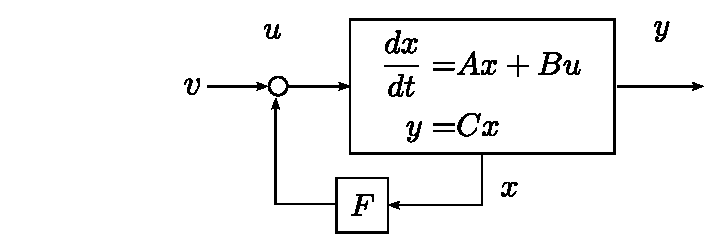
\includegraphics{sfigure/feedback.eps} 
  \caption{状態フィードバック}
  \label{fig_state_feedback}
 \end{center}
\end{figure}
\end{frame}


%%%%%%%%%%%%%%%%%%%%%%%%%%%%%%%%%%%%%%%%%%%%%%%%%%%%%%%%%%%%%%
\begin{frame}[t]
\frametitle{1.9 状態フィードバック (極配置問題)}
%-------------------------------------------------------------
\begin{block}{\bf 極配置(pole assignment)問題}
フィードバック行列$F$を選ぶことにより，閉ループ系の極を（任意の）指定された値
にする問題
\end{block}

閉ループ系の望ましい極
を$p_1, p_2, \cdots, p_n$ として，\\
$(A + B F)$の特性多項式が
\begin{align}
 \det (s I - (A + B F))
 &= (s - p_1)(s - p_2) \cdots (s - p_n) \nonumber \\
 &\defeq s^n + \mu_{n-1} s^{n-1} + \mu_{n-2} s^{n-2}
  + \cdots + \mu_1 s^1 + \mu_0
\end{align}
となるような\Blue{$F$を求める問題}となる．

\vspace{5mm}

ここで$\mu_i$が実数となるように$p_i$
が選ばれていると仮定する．
\footnote{これは$p_i = \xi_i + j \eta_i $であり$\eta_i
\neq 0$であるならば$p_j = \xi_i - j \eta_i$も指定された極に含まれてい
るという仮定}

この問題は\underline{\Blue{\bf 可制御なシステムについて可解}}となることが知られている．

\end{frame}


%%%%%%%%%%%%%%%%%%%%%%%%%%%%%%%%%%%%%%%%%%%%%%%%%%%%%%%%%%%%%%
\begin{frame}[t]
\frametitle{1.9 状態フィードバック (簡単なシステムの極配置)}
%-------------------------------------------------------------
例)
\begin{equation}
 \frac{d}{dt}
 \left(
 \begin{array}{c}
  x_1 \\
  x_2
 \end{array}
 \right) =
 \left(
 \begin{array}{cc}
  0 & 1\\
  1 & 1
 \end{array}
 \right)
 \left(
 \begin{array}{c}
  x_1 \\
  x_2
 \end{array}
 \right) +
 \left(
 \begin{array}{c}
  0 \\
  1
 \end{array}
 \right) u
\end{equation}
で表されるシステムの極を$-1, -2$とする\Blue{状態フィードバック$F$} を求める．
$u = Fx = (\begin{array}{cc}f_1 & f_2\end{array})x$とすると，
\begin{align}
 \frac{d}{dt}
 \left(
 \begin{array}{c}
  x_1 \\
  x_2
 \end{array}
 \right)
 &=
 \left(
 \begin{array}{cc}
  0 & 1\\
  1 & 1
 \end{array}
 \right)
 \left(
 \begin{array}{c}
  x_1 \\
  x_2
 \end{array}
 \right) +
 \left(
 \begin{array}{c}
  0 \\
  1
 \end{array}
 \right)
 \left(
 \begin{array}{cc}
  f_1 & f_2
 \end{array}
 \right)
 \left(
 \begin{array}{c}
  x_1 \\
  x_2
 \end{array}
 \right)
\nonumber \\
 &=
 \left(
 \begin{array}{cc}
  0 & 1\\
  1 & 1
 \end{array}
 \right)
 \left(
 \begin{array}{c}
  x_1 \\
  x_2
 \end{array}
 \right) +
 \left(
 \begin{array}{cc}
  0   & 0 \\
  f_1 & f_2
 \end{array}
 \right)
 \left(
 \begin{array}{c}
  x_1 \\
  x_2
 \end{array}
 \right)
\nonumber \\
 &=
 \left(
 \begin{array}{cc}
  0 & 1 \\
  1 + f_1 & 1 + f_2
 \end{array}
 \right)
 \left(
 \begin{array}{c}
  x_1 \\
  x_2
 \end{array}
 \right)
\end{align}
となるので，フィードバック系の特性多項式は以下のようになる．
\end{frame}


%%%%%%%%%%%%%%%%%%%%%%%%%%%%%%%%%%%%%%%%%%%%%%%%%%%%%%%%%%%%%%
\begin{frame}[t]
\frametitle{1.9 状態フィードバック (簡単なシステムの極配置)}
%-------------------------------------------------------------

フィードバック系の特性多項式は以下のようになる．
\begin{equation}
 \det(sI - (A + BF)) =
  \det \left (
    \begin{array}{cc}
      s & -1 \\
      -(1+f_1) & s-(1+f_2)
    \end{array}
  \right )
  = s^2 - (1 + f_2) s - (1 + f_1)
\end{equation}
一方，望ましいフィードバック系の特性多項式は
\begin{equation}
 (s + 1)(s + 2) = s^2 + 3 s + 2
\end{equation}
係数を比較することで，
$F = (\begin{array}{cc}f_1 & f_2\end{array}) =
(\begin{array}{cc}-3 & -4\end{array})$となる．
\end{frame}


%%%%%%%%%%%%%%%%%%%%%%%%%%%%%%%%%%%%%%%%%%%%%%%%%%%%%%%%%%%%%%
\begin{frame}[t]
\frametitle{1.9 状態フィードバック ＜演習＞極配置}
%-------------------------------------------------------------
次の状態方程式
\begin{align*}
  \frac{d}{dt}
  \left (
  \begin{array}{c}
   x_1 \\ x_2
  \end{array}
  \right )
  & =
  \left (
  \begin{array}{cc}
   0 & 1 \\
   0 & -1
  \end{array}
  \right )
  \left (
  \begin{array}{c}
   x_1 \\ x_2
  \end{array}
  \right )
  +
  \left (
  \begin{array}{c}
   0 \\ 1
  \end{array}
  \right )
  u
\end{align*}
に対して閉ループ系の極が$-4,-5$となるような状態フィードバック
\begin{align*}
  u
  &=
  \left (
  \begin{array}{cc}
   f_1 & f_2
  \end{array}
  \right )
  \left (
  \begin{array}{c}
   x_1 \\ x_2
  \end{array}
  \right )
\end{align*}
を求めよ．
\end{frame}

%%%%%%%%%%%%%%%%%%%%%%%%%%%%%%%%%%%%%%%%%%%%%%%%%%%%%%%%%%%%%%
\begin{frame}[t]
\frametitle{1.9 状態フィードバック (極配置の数値解)}
%-------------------------------------------------------------
\vspace*{30mm}

科学技術計算ソフトウェア(MATLAB$^{\tiny \textregistered}$ (http://jp.mathworks.com/)など)の普及により，多入力系も含めて極配置問題の数値解が容易に得られるようになっている．

\end{frame}

%%%%%%%%%%%%%%%%%%%%%%%%%%%%%%%%%%%%%%%%%%%%%%%%%%%%%%%%%%%%%%
\begin{frame}[t]
\frametitle{1.9 状態フィードバック (1入力可制御正準形の極配置)}
%-------------------------------------------------------------
極配置問題は一入力可制御な系に対しては簡単に解ける．\\
ここでは
\Blue{一入力可制御正準形で表されたシステムの極配置問題の解法}を与える．

次の可制御正準形で表されたシステムを考える．
\begin{align}
 \frac{d}{dt}
  \left(\begin{array}{c}
         x_1 \\
   x_2 \\
   \vdots \\
   x_{n-1} \\
   x_n
  \end{array}\right)
  &=
  \left(\begin{array}{ccccc}
     0      & 1      & 0      & \cdots & 0 \\
   0      & 0      & 1      & \ddots & \vdots \\
   \vdots & \vdots & \ddots & \ddots & 0 \\
   0      & 0      & \cdots & 0      & 1 \\
   -a_0   & -a_1   & \cdots & -a_{n-2} & -a_{n-1}
  \end{array}\right)
  \left(\begin{array}{c}
   x_1 \\
   x_2 \\
   \vdots \\
   x_{n-1} \\
   x_n
  \end{array}\right)
  +
  \left(\begin{array}{c}
         0 \\
   0 \\
   \vdots \\
   0 \\
   1
  \end{array}\right)
  u
\end{align}
このシステムの$A$行列の特性多項式は$A$行列の最下列の値を用いて
\begin{equation}
 \det (sI-{A}) = s^n + a_{n-1} s^{n-1}
  + a_{n-2} s^{n-2} + \cdots + a_1 s + a_0
\end{equation}
と与えられる．

\end{frame}


%%%%%%%%%%%%%%%%%%%%%%%%%%%%%%%%%%%%%%%%%%%%%%%%%%%%%%%%%%%%%%
\begin{frame}[t]
\frametitle{1.9 状態フィードバック (1入力可制御正準形の極配置)}
%-------------------------------------------------------------
状態フィードバックとして
\small{
\begin{align}
 u = F x =
 (f_1, f_2, \cdots, f_{n-1}, f_{n})
 \left(\begin{array}{c}
        x_1 \\
    x_2 \\
    \vdots \\
    x_{n-1} \\
    x_n
       \end{array}\right)
\end{align}
}
を用いると，状態方程式は
\small{
\begin{align}
 \frac{d}{dt}
  \left(\begin{array}{c}
         x_1 \\
   x_2 \\
   \vdots \\
   x_{n-1} \\
   x_n
  \end{array}\right)
  &=
  \left(\begin{array}{ccccc}
     0      & 1      & 0      & \cdots & 0 \\
   0      & 0      & 1      & \ddots & \vdots \\
   \vdots & \vdots & \ddots & \ddots & 0 \\
   0      & 0      & \cdots & 0      & 1 \\
   f_1-a_0   & f_2 -a_1   & \cdots & f_{n-1} -a_{n-2} & f_{n} -a_{n-1}
  \end{array}\right)
  \left(\begin{array}{c}
   x_1 \\
   x_2 \\
   \vdots \\
   x_{n-1} \\
   x_n
  \end{array}\right)
\end{align}
}
となり，その$A+BF$の特性多項式は
次式となる．
\begin{equation}
 \det (sI-\Blue{(A+BF)}) = s^n + \Blue{(a_{n-1}-f_n)} s^{n-1}
  + \Blue{(a_{n-2}-f_{n-1})} s^{n-2} + \cdots 
  + \Blue{(a_0-f_1)}
\label{eq:poleas_cha1}
\end{equation}
\end{frame}


%%%%%%%%%%%%%%%%%%%%%%%%%%%%%%%%%%%%%%%%%%%%%%%%%%%%%%%%%%%%%%
\begin{frame}[t]
\frametitle{1.9 状態フィードバック (1入力可制御正準形の極配置)}
%-------------------------------------------------------------
$A+BF$の特性多項式
\begin{equation}
 \det (sI-\Blue{(A+BF)}) = s^n + \Blue{(a_{n-1}-f_n)} s^{n-1}
  + \Blue{(a_{n-2}-f_{n-1})} s^{n-2} + \cdots 
  + \Blue{(a_0-f_1)}
\tag{\ref{eq:poleas_cha1}}
\end{equation}
その一方，\\
\Blue{$p_1, p_2, \cdots, p_n$} : システムの望ましいシステムの極($A+BF$の極)\\
に対して
\begin{align}
 \det (s I - A - B F)
 &= (s - p_1)(s - p_2) \cdots (s - p_n) \nonumber \\
 &\defeq s^n + \mu_{n-1} s^{n-1} + \mu_{n-2} s^{n-2}
  + \cdots + \mu_1 s^1 + \mu_0
\label{eq:poleas_cha2}
\end{align}
と$\mu_i$をおくと，係数比較より
\begin{align}
 \mu_0 & = a_0-f_1    \nonumber\\
 \mu_{1} & = a_1-f_2  \nonumber\\
 \vdots \\
 \mu_{n-2} & = a_{n-2}-f_{n-1} \nonumber\\
 \mu_{n-1} & = a_{n-1}-f_n    \nonumber
\end{align}
\end{frame}


%%%%%%%%%%%%%%%%%%%%%%%%%%%%%%%%%%%%%%%%%%%%%%%%%%%%%%%%%%%%%%
\begin{frame}[t]
\frametitle{1.9 状態フィードバック (1入力可制御正準形の極配置)}
%-------------------------------------------------------------
\vspace*{-5mm}

\begin{align}
 \mu_0 & = a_0-f_1    \nonumber\\
 \mu_{1} & = a_1-f_2  \nonumber\\
 \vdots \\
 \mu_{n-1} & = a_{n-1}-f_n    \nonumber
\end{align}
これを$f_i$について解いたもの
\begin{align}
 f_1 & = a_0-\mu_0
\nonumber\\
 f_2 & = a_1-\mu_{1}
\nonumber\\
 \vdots
\nonumber\\
 f_n& = a_{n-1}-\mu_{n-1}
\nonumber
\end{align}
とすれば極配置問題が解けたことになる．\\
これを$F$行列で表せば
次式となる．
\begin{equation}
 {F} = \left(\begin{array}{cccc}
            a_0-\mu_0, & a_1-\mu_1, & \cdots, & a_{n-1}-\mu_{n-1}
     \end{array}\right)
\end{equation}

\end{frame}


%%%%%%%%%%%%%%%%%%%%%%%%%%%%%%%%%%%%%%%%%%%%%%%%%%%%%%%%%%%%%%
\begin{frame}[t]
\frametitle{1.9 状態フィードバック (極と応答)}
%-------------------------------------------------------------
複素係数を持つ1次のシステムを考える．
\begin{align}
 \dot{x} &= \lambda \ x \nonumber \\
         &= (\alpha + j \beta) x
\end{align}
このシステムの%極は明らかに$\alpha + j\beta$であるから，
極の実部は$\alpha$，
極の虚部は$\beta$である．\\
また，この微分方程式を解けばシステムの応答は
\begin{align}
 x(t) &= e^{(\alpha + j \beta)t} x(0) \nonumber \\
      &= e^{\alpha t}\alert{e^{j \beta t}} x(0) \\
      &= e^{\alpha t} \alert{\{ \cos(\beta t) + j \sin(\beta t) \} }x(0)
      \ \ \ \ \ \ \text{(\alert{オイラーの公式}より)} \\
      &= e^{\alpha t} \cos(\beta t) x(0) + j e^{\alpha t} \sin(\beta t)x(0)
\end{align}
となる．\\
極とシステムの応答の関係を直感的に理解するためには，$x(0)=1$の場合の応
答の{実部}，つまり
\begin{equation}
 x(t) = e^{\alpha t} \cos(\beta t)
\end{equation}
について検討すれば十分である．\\
$\Longrightarrow$ \Blue{$\alpha$と$\beta$の大きさによるシステムの応答の違いはどうだろうか?}
\end{frame}


%%%%%%%%%%%%%%%%%%%%%%%%%%%%%%%%%%%%%%%%%%%%%%%%%%%%%%%%%%%%%%
\begin{frame}[t]
\frametitle{1.9 状態フィードバック (極と応答)}
%-------------------------------------------------------------
$x(0)=1$の場合の応答の{実部}
\addtocounter{equation}{-1}
\begin{equation}
 x(t) = e^{\alpha t} \cos(\beta t)
\end{equation}

\begin{itemize}
 \item $\alpha$は極の実部に，$\beta$は極の虚部に対応している．
 \item $\alpha>0$のときは$e^{\alpha t}$は発散，$\alpha<0$のときは
       $e^{\alpha t}$は$0$に収束する．
 \item $\alpha$が小さいほど(負で絶対値が大きいほど)$e^{\alpha t}$は速
       く０に収束する．
 \item $\beta$が大きいほど$\cos(\beta t)$の振動が速くなる．
 \item $e^{\alpha t}$と$ \cos(\beta t)$を乗じたものがシステムの応答になる．
\end{itemize}
\end{frame}


%%%%%%%%%%%%%%%%%%%%%%%%%%%%%%%%%%%%%%%%%%%%%%%%%%%%%%%%%%%%%%
\begin{frame}[t]
\frametitle{1.9 状態フィードバック (極と応答)}
%-------------------------------------------------------------
$\left\{\parbox{7zw}{
\begin{tabular}{l}
 $\alpha=0.5, -1, -5$ \\
 $\beta=2, 10$
\end{tabular}}\right.$
~としたときの$e^{\alpha t}$と$\cos(\beta t)$の時間応答

\begin{figure}[t!]
 \begin{minipage}{0.5\textwidth}
  \begin{center}
   \scalebox{.8}{\input{../figure/fig1.pstex_t}}
   (a) $e^{\alpha t}$
  \end{center}
 \end{minipage}%
 \begin{minipage}{0.5\textwidth}
  \begin{center}
   \scalebox{.8}{\input{../figure/fig2.pstex_t}}
   (b) $\cos \beta t$
  \end{center}
 \end{minipage}
 \caption{極と応答1}
 \label{fig_pole12}
\end{figure}

\end{frame}


%%%%%%%%%%%%%%%%%%%%%%%%%%%%%%%%%%%%%%%%%%%%%%%%%%%%%%%%%%%%%%
\begin{frame}[t]
\frametitle{1.9 状態フィードバック (極と応答)}
%-------------------------------------------------------------
\begin{figure}[t!]
 \begin{minipage}{0.5\textwidth}
  \begin{center}
   \scalebox{.8}{\input{../figure/fig3a.pstex_t}}
   (a) $\alpha = 0.5$
  \end{center}
 \end{minipage}%
 \begin{minipage}{0.5\textwidth}
  \begin{center}
   \scalebox{.8}{\input{../figure/fig3b.pstex_t}}
   (b) $\alpha = -1$
  \end{center}
 \end{minipage}
 \caption{極と応答2 $(\beta = 10)$}
 \label{fig_pole34}
\end{figure}

$\alpha > 0$ のときは応答が発散し，
$\alpha < 0$ のときは安定. \\

$\Longrightarrow$ \Blue{\bf 極の実部が負のときシステムは安定(正のときは不安定)である}


\end{frame}


%%%%%%%%%%%%%%%%%%%%%%%%%%%%%%%%%%%%%%%%%%%%%%%%%%%%%%%%%%%%%%
\begin{frame}[t]
\frametitle{1.9 状態フィードバック (極と応答)}
%-------------------------------------------------------------
\begin{figure}[t!]
 \begin{minipage}{0.5\textwidth}
  \begin{center}
   \scalebox{.8}{\input{../figure/fig4a.pstex_t}}
   (a) $\alpha = -1$
  \end{center}
 \end{minipage}%
 \begin{minipage}{0.5\textwidth}
  \begin{center}
   \scalebox{.8}{\input{../figure/fig4b.pstex_t}}
   (b) $\alpha = -5$
  \end{center}
 \end{minipage}
 \caption{極と応答3 $(\beta = 2)$}
 \label{fig_pole56}
\end{figure}
$e^{\alpha t}$の収束の速さに引きずられて$\alpha=-5$のときの方が収束が速くなっている．
$\Longrightarrow$ \Blue{\bf 極の実部が小さいほど(負で絶対値が大きいほど)応答が速く0に収束する}

\end{frame}


%%%%%%%%%%%%%%%%%%%%%%%%%%%%%%%%%%%%%%%%%%%%%%%%%%%%%%%%%%%%%%
\begin{frame}[t]
\frametitle{1.9 状態フィードバック (極と応答)}
%-------------------------------------------------------------
\begin{figure}[t!]
 \begin{minipage}{0.5\textwidth}
  \begin{center}
   \scalebox{.8}{\input{../figure/fig5a.pstex_t}}
   (a) $\beta = 2$
  \end{center}
 \end{minipage}%
 \begin{minipage}{0.5\textwidth}
  \begin{center}
   \scalebox{.8}{\input{../figure/fig5b.pstex_t}}
   (b) $\beta = 10$
  \end{center}
 \end{minipage}
 \caption{極と応答4 ($\alpha = -1$)}
 \label{fig_pole78}
\end{figure}
収束の速さは同じであるが，$\beta$が大きい方が応答が振動的になる．\\
$\Longrightarrow$ \Blue{\bf 極の虚部が大きくなるほど応答が振動的になる.}
\end{frame}


%%%%%%%%%%%%%%%%%%%%%%%%%%%%%%%%%%%%%%%%%%%%%%%%%%%%%%%%%%%%%%
\begin{frame}[t]
\frametitle{1.9 状態フィードバック (極と応答)}
%-------------------------------------------------------------
\begin{figure}[t!]
 \begin{minipage}{0.5\textwidth}
  \begin{center}
   \scalebox{.8}{\input{../figure/fig6a.pstex_t}}
   (a) $\alpha = -1, \beta = 2$
  \end{center}
 \end{minipage}%
 \begin{minipage}{0.5\textwidth}
  \begin{center}
   \scalebox{.8}{\input{../figure/fig6b.pstex_t}}
   (b) $\alpha = -5, \beta = 10$
  \end{center}
 \end{minipage}
 \caption{極と応答5}
 \label{fig_pole910}
\end{figure}
原点への収束はもちろん$\alpha = -5$の方が速いが，
オーバーシュートはほとんど同じである.\\
$\Longrightarrow$ \Blue{\bf システムの振動性が極の実部と虚部の比で決定される.}

\end{frame}


%%%%%%%%%%%%%%%%%%%%%%%%%%%%%%%%%%%%%%%%%%%%%%%%%%%%%%%%%%%%%%
\begin{frame}[t]
\frametitle{1.9 状態フィードバック (極と応答)}
%-------------------------------------------------------------
さらに，極配置法を用いて制御系を設計する場合には\\
\Blue{\bf 応答を速くする(閉ループ系の極の実部を小さくする)と入力が大きくなる}\\
ことに注意して極端に応答を速くしないことが必要．

\vspace{5mm}

以上，極とシステムの応答の関係をまとめると ...
\begin{enumerate}
  \item 極の\structure{実部が負}のときシステムは安定(正のときは不安定)である
  \item 極の\structure{実部が小さい}ほど(負で絶対値が大きいほど)応答が速く0に収束する
  \item 極の\structure{虚部が大きく}なるほど応答が振動的になる
  \item システムの振動性が極の\structure{実部と虚部の比}で決定される
  \item \structure{応答を速く}する(閉ループ系の極の実部を小さくする)と入力が大きくなる
\end{enumerate}

\end{frame}


%%%%%%%%%%%%%%%%%%%%%%%%%%%%%%%%%%%%%%%%%%%%%%%%%%%%%%%%%%%%%%
\begin{frame}[t]
\frametitle{1.9 状態フィードバック (極と応答)}
%-------------------------------------------------------------
これらを念頭に置いて，
極配置を行うときはFig.\ref{fig_pole}のような範囲に
極を配置することが良いとされている．
\begin{figure}
 \begin{center}
  \input{../figure/pole.pstex_t}
  \caption{望ましい極配置}
  \label{fig_pole}
 \end{center}
\end{figure}
\end{frame}


%%%%%%%%%%%%%%%%%%%%%%%%%%%%%%%%%%%%%%%%%%%%%%%%%%%%%%%%%%%%%%
\begin{frame}[t]
\frametitle{1.9 状態フィードバック (最適制御)}
%-------------------------------------------------------------
安定化フィードバックを極配置により求める方法を示した．\\
しかし，多入力系の場合にはフィードバックが一意に決まらない．

例）
\[
 \frac{d}{dt}
 \left(
 \begin{array}{c}
  x_1 \\
  x_2
 \end{array}
 \right) =
 \left(
 \begin{array}{cc}
  1 & 0 \\
  0 & 1
 \end{array}
 \right)
 \left(
 \begin{array}{c}
  x_1 \\
  x_2
 \end{array}
 \right) +
 \left(
 \begin{array}{cc}
  1 & 0 \\
  0 & 1
 \end{array}
 \right)
 \left(
 \begin{array}{c}
  u_1 \\
  u_2
 \end{array}
 \right)
\]
で表されるシステムに対して，
\begin{align*}
 u &=
 \left(
 \begin{array}{cc}
  -2 & 0 \\
  0 & -3
 \end{array}
 \right)
 \left(
 \begin{array}{c}
  x_1 \\
  x_2
 \end{array}
 \right) \text{のとき，}\\
 & \quad
 \det(sI - (A + BF)) =
 \det\left(
 \begin{array}{cc}
  s+1 & 0 \\
  0 & s+2
 \end{array}
 \right)
 = \Blue{s^2 + 3s + 2} \\[5mm]
 u &=
 \left(
 \begin{array}{cc}
  -3 & 0 \\
  0 & -2
 \end{array}
 \right)
 \left(
 \begin{array}{c}
  x_1 \\
  x_2
 \end{array}
 \right)\text{のとき，}\\
 & \quad
 \det(sI - (A + BF)) =
 \det\left(
 \begin{array}{cc}
  s+2 & 0 \\
  0 & s+1
 \end{array}
 \right)
 = \Blue{s^2 + 3s + 2} \\[5mm]
\end{align*}
\end{frame}


%%%%%%%%%%%%%%%%%%%%%%%%%%%%%%%%%%%%%%%%%%%%%%%%%%%%%%%%%%%%%%
\begin{frame}[t]
\frametitle{1.9 状態フィードバック (最適制御)}
%-------------------------------------------------------------
\begin{align*}
 u &=
 \left(
 \begin{array}{cc}
  -1 & 1 \\
  -2 & -4
 \end{array}
 \right)
 \left(
 \begin{array}{c}
  x_1 \\
  x_2
 \end{array}
 \right) \text{のとき，}\\
 & \quad
 \det(sI - (A + BF)) =
 \det\left(
 \begin{array}{cc}
  s & -1 \\
  2 & s+3
 \end{array}
 \right)
 = \Blue{s^2 + 3s + 2}
\end{align*}
のように，\\
\Blue{異なるフィードバック行列に対し，フィードバック系の極が全て$-1, -2$となる}．
つまり，極を指定してもどのフィードバック行列を用いればいいのかわからないことになる．
\end{frame}


%%%%%%%%%%%%%%%%%%%%%%%%%%%%%%%%%%%%%%%%%%%%%%%%%%%%%%%%%%%%%%
\begin{frame}[t]
\frametitle{1.9 状態フィードバック (最適制御)}
%-------------------------------------------------------------
安定化フィードバックを次の\Blue{２次形式評価関数}を
最小にするように選ぶ方法\\
(\Blue{最適フィードバック})がある．
\begin{equation}
 J = \int_{0}^{\infty} (x^T Q x + u^T R u) dt
\label{eqn:P-index}
\end{equation}
$Q$ : 半正定($Q = H^T H$で表わされる)\\
$R$ : 正定($R = L^T L$, ($L$
は正則行列)で表わせる)

\hspace{5mm}

この$J$を最小にするフィードバックは，$P$を
Riccati方程式
\begin{equation}
 A^T P + P A - P B R^{-1} B^T P + Q = 0
\end{equation}
の正定解として
\begin{equation}
   u = - R^{-1} B^T P x \defeq Fx
\end{equation}
で表わされる．\\
さらに$(H,A)$が可観測であれば閉ループ系が安定になる．
\end{frame}


%%%%%%%%%%%%%%%%%%%%%%%%%%%%%%%%%%%%%%%%%%%%%%%%%%%%%%%%%%%%%%
\begin{frame}[t]
\frametitle{1.9 状態フィードバック (最適制御)}
%-------------------------------------------------------------
$Q(=H^T H)$と$R(=L^T L)$は以下のように選ばれることが多い．
\begin{equation}
 H = \left(\begin{array}{cccc}
            h_1    & 0   & \cdots & 0 \\
      0      & h_2 &        & 0 \\
      \vdots &     & \ddots & \\
      0      & 0   &        & h_n
     \end{array}\right)
 , \quad
 L = \left(\begin{array} {cccc}
            l_1    & 0   & \cdots & 0 \\
      0      & l_2 &        & 0 \\
      \vdots &     & \ddots & \\
      0      & 0   &        & l_m
     \end{array}\right)
\end{equation}
($h_i>0$, $l_j>0$).
\end{frame}


%%%%%%%%%%%%%%%%%%%%%%%%%%%%%%%%%%%%%%%%%%%%%%%%%%%%%%%%%%%%%%
\begin{frame}[t]
\frametitle{1.9 状態フィードバック (最適制御)}
%-------------------------------------------------------------
このとき，$x = (x_1, x_2, \cdots, x_n)^T$, $u = (u_1, u_2, \cdots, u_m)^T$とすれば評価関数は，
{\footnotesize
\begin{align}
 J
 &= \int_{0}^{\infty} (x^T Q x + u^T R u) dt \nonumber \\
 &= \int_{0}^{\infty} (x^T H^TH x + u^T L^TL u) dt \nonumber \\
 &= \int_{0}^{\infty} ((Hx)^TH x + (Lu)^TL u) dt \nonumber \\
 &= \int_{0}^{\infty}
    \left\{
    \left(
    \begin{array}{cccc}
     h_1x_1 & \cdots & h_nx_n
    \end{array}
    \right)
    \left(
    \begin{array}{c}
     h_1x_1 \\
     h_2x_2 \\
     \vdots \\
     h_nx_n
    \end{array}
    \right) +
    \left(
    \begin{array}{cccc}
     l_1u_1 & \cdots & l_mu_m
    \end{array}
    \right)
    \left(
    \begin{array}{c}
     l_1u_1 \\
     l_2u_2 \\
     \vdots \\
     l_mu_m
    \end{array}
    \right)
    \right\}dt \nonumber \\
 &= \int_0^{\infty} (h_1^2 x_1^2 + h_2^2 x_2^2 + \cdots +
     h_n^2 x_n^2 + l_1^2 u_1^2 + \cdots + l_m^2 u_m^2)dt
\label{eqn:P-index2}
\end{align}
}
となる．この評価関数の意味について考えてみよう．
\end{frame}


%%%%%%%%%%%%%%%%%%%%%%%%%%%%%%%%%%%%%%%%%%%%%%%%%%%%%%%%%%%%%%
\begin{frame}[t]
\frametitle{1.9 状態フィードバック (最適制御)}
%-------------------------------------------------------------
\vspace*{-5mm}

\begin{align}
 J
 &= \int_0^{\infty} (h_1^2 x_1^2 + h_2^2 x_2^2 + \cdots +
     h_n^2 x_n^2 + l_1^2 u_1^2 + \cdots + l_m^2 u_m^2)dt
\tag{\ref{eqn:P-index2}}
\end{align}
\begin{columns}[t]
\begin{column}{0.4\textwidth}
評価関数(\ref{eqn:P-index2})の第１項として以下の部分を考える．
\begin{align}
  J' &= \int_0^\infty x_1^2 dt
\end{align}
これと同じようなものとして次の絶対値積分を考える．
\begin{align}
  J'' &= \int_0^\infty | x_1 | \ dt
\end{align}
\end{column}
\begin{column}{0.05\textwidth}

\end{column}
\begin{column}{0.5\textwidth}
\begin{figure}
 \begin{center}
  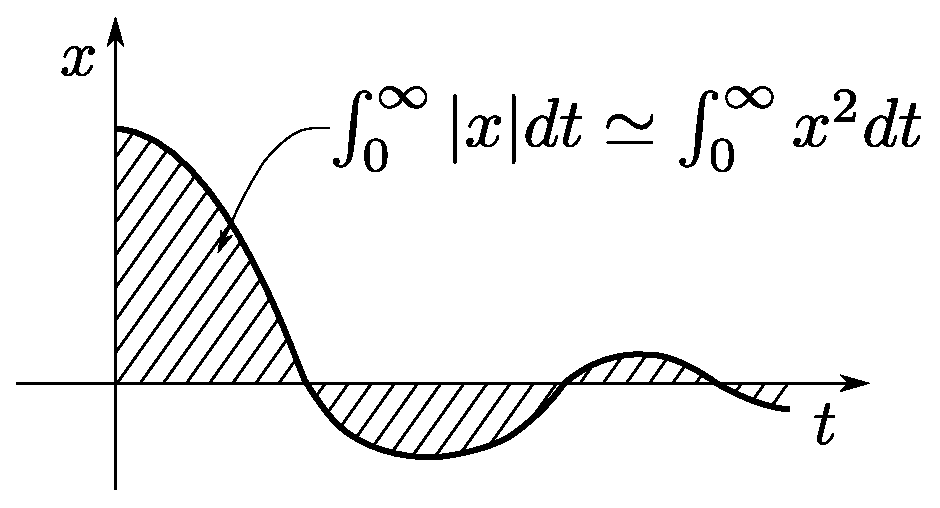
\includegraphics[width=0.9\linewidth]{sfigure/optimal.eps}
  \caption{評価関数のイメージ}
  \label{fig_J}
 \end{center}
\end{figure}
\end{column}
\begin{column}{0.05\textwidth}

\end{column}
\end{columns}
\vspace{5mm}
これはFig~\ref{fig_J}の斜線部分の面積に相当する．\\
評価関数$J''$を最小化
$\Longrightarrow$ 斜線の面積を最小化
$\Longrightarrow$ \Blue{$x$を速く$0$に収束} \\
\Blue{$J'$の最小化}も同等の効果がある．
\end{frame}


%%%%%%%%%%%%%%%%%%%%%%%%%%%%%%%%%%%%%%%%%%%%%%%%%%%%%%%%%%%%%%
\begin{frame}[t]
\frametitle{1.9 状態フィードバック (最適制御)}
%-------------------------------------------------------------
評価関数
\begin{align}
 J
 &= \int_{0}^{\infty} (x^T Q x + u^T R u) dt \nonumber \\
 &= \int_0^{\infty} (h_1^2 x_1^2 + h_2^2 x_2^2 + \cdots +
     h_n^2 x_n^2 + l_1^2 u_1^2 + \cdots + l_m^2 u_m^2)dt
\tag{\ref{eqn:P-index2}}
\end{align}

一方，\\
同様に評価関数(\ref{eqn:P-index2})の$u_j$に関する項を最小化
$\Longrightarrow$ 入力を極力使わない．

\vspace{5mm}

このように，\\
\Blue{評価関数(\ref{eqn:P-index2})を最小化する\\
$\Longrightarrow$ できるだけ入力$u$を用いずに，できるだけ速く$x$を$0$に収束する\\}という問題設定を考えることができる．\\
それぞれの項の重みづけが$h_i$, $l_j$ ($Q$, $R$)ということになる．
\end{frame}


%%%%%%%%%%%%%%%%%%%%%%%%%%%%%%%%%%%%%%%%%%%%%%%%%%%%%%%%%%%%%%
\begin{frame}[t]
\frametitle{1.9 状態フィードバック (最適制御)}
%-------------------------------------------------------------
評価関数
\begin{align}
 J
 &= \int_{0}^{\infty} (x^T Q x + u^T R u) dt \nonumber \\
 &= \int_0^{\infty} (h_1^2 x_1^2 + h_2^2 x_2^2 + \cdots +
     h_n^2 x_n^2 + l_1^2 u_1^2 + \cdots + l_m^2 u_m^2)dt
\tag{\ref{eqn:P-index2}}
\end{align}

実際の設計時における\Blue{$Q=H^TH$, $R=L^TL$は試行錯誤で選ぶ}こととなるが，\\
次のような方針で望ましい応答を容易に得ることができる．

\vspace{5mm}

ある$H$, $L$に対する閉ループ系の応答の
$x_1$が大きくふれすぎる．\\
$\Longrightarrow$ \Blue{$h_1$を大きくして再設計}\\
$\Longrightarrow$ \Blue{$J$に対する$x_1$の寄与が大きく}なり，$J$を小さくするためには$x_1$を小さくしなければならない．\\
$\Longrightarrow$ 結果的に\Blue{$x_1$をおさえる制御系が設計できる}．\\

\vspace{3mm}

同様に$x_i$と$u_j$の挙動が激しい(大きく動く)ならば$h_i$と$l_j$を
大きくすれば$x_i$, $u_j$の動きが抑えられる．

通常，$h_i^2$, $l_j^2$の増減は$10$倍，$1/10$を目安にすることが多い．つまり，$1$の次は$10$, その次は$100$であり，$1$の前は$1/10$として調整することが多い．

\end{frame}

%%%%%%%%%%%%%%%%%%%%%%%%%%%%%%%%%%%%%%%%%%%%%%%%%%%%%%%%%%%%%%
\begin{frame}[t]
\frametitle{1.9 状態フィードバック ＜演習＞最適制御}
%-------------------------------------------------------------



\noindent
{\bf ＜演習＞最適制御：不安定極} \nopagebreak

次のシステムと評価関数に対する最適制御を求めよ．
\begin{align*}
	\frac{dx}{dt} & = 1 \cdot x + 1 \cdot u \ \ \ \ \ \ \ \ \ \ \ \ A=1,B=1\\
	J & = \int_0^{\infty} x^2 + r u^2 dt \ \ \ \ \ \ \ \ Q=1,R=r
\end{align*}
また，$r\rightarrow 0$と$r\rightarrow \infty$の場合の入力とフィードバック系の極を求めよ．
\\[5mm]

\noindent
{\bf ＜演習＞最適制御：安定極} \nopagebreak

次のシステムと評価関数に対する最適制御を求めよ．
\begin{align*}
	\frac{dx}{dt} & = \underline{-1} \cdot x + 1 \cdot u \ \ \ \ \ \ \ \ \ \ \ \ A=\underline{-1},B=1\\
	J & = \int_0^{\infty} x^2 + r u^2 dt \ \ \ \ \ \ \ \ Q=1,R=r
\end{align*}
また，$r\rightarrow 0$と$r\rightarrow \infty$の場合の入力とフィードバック系の極を求めよ．

\end{frame}



%%%%%%%%%%%%%%%%%%%%%%%%%%%%%%%%%%%%%%%%%%%%%%%%%%%%%%%%%%%%%%
\begin{frame}[t]
\frametitle{1.9 状態フィードバック (Riccati方程式の解法)}
%-------------------------------------------------------------

有本-Potterの方法：行列$\Phi$を次のように定義する．
\begin{align}
 \Phi = \left(\begin{array}{cc}
	       A  & - B R^{-1} B^T \\
	       -Q & - A^T
	      \end{array}\right)
\end{align}
この$\Phi$の固有値のうち実部が負のものが$n$個あることが分かっている．これらの固有値を$\lambda_i$, $i=1,2,\cdots,n$とし，これに対応する固有ベクトルを$w_1, w_2, \cdots, w_n$する．この固有ベクトルを次のように分解しておく．
\begin{align}
 w_i = \left(\begin{array}{c}
	      \xi_i \\
	      \eta_i
	     \end{array}\right), \hspace{1cm} \xi_i \in {\mathbb R}^n, \ \eta_i \in {\mathbb R}^n
\end{align}
このとき
\begin{align}
	P = Y X^{-1}, \ \ \ 
	X = (\xi_1, \xi_2, \cdots, \xi_n), \ \ \ 
	Y = (\eta_1, \eta_2, \cdots, \eta_n)
\end{align}
と選べば$P$は正定かつRiccati方程式を満たすことが知られている．

\end{frame}



%%%%%%%%%%%%%%%%%%%%%%%%%%%%%%%%%%%%%%%%%%%%%%%%%%%%%%%%%%%%%%
\begin{frame}[t]
\frametitle{1.9 状態フィードバック (Riccati方程式の解法)}
%-------------------------------------------------------------
Riccati方程式の解法としては，これ以外にLMI(線形行列不等式)を用いた方法などがある．
\\[2cm]

科学技術計算ソフトウェア(MATLAB$^{\tiny \textregistered}$ (http://jp.mathworks.com/)など)の普及により，最適フィードバックの数値解が容易に得られるようになっている．

\end{frame}

%%%%%%%%%%%%%%%%%%%%%%%%%%%%%%%%%%%%%%%%%%%%%%%%%%%%%%%%%%%%%%
\begin{frame}[t]
\frametitle{1.9 状態フィードバック \\ (リアプノフ関数とシステムの安定性)}
%-------------------------------------------------------------
正則行列$T$(と$P=T^T T$)を用いてつぎのスカラー関数を考える．
\begin{equation}
 V(x) = x^T T^T T x = x^T P x
\end{equation}
これは座標変換された状態ベクトル
\begin{equation}
 \bar{x} = T x
\end{equation}
に対して
\begin{equation}
 V(x) = \bar{x}^T \bar{x} = | \bar{x} | ^2
\end{equation}
に相当する．\\
$\Longrightarrow$ $V(x) \geq 0$でかつ$V(x) = 0$となるのは$x=0$
, ($\bar{x} = 0 $)のみ\\
このような$V(x)$のことを\Blue{\bf 正定関数(Positive Definite Function)}，\\
$P$のことを\Blue{\bf 正定行列(Positive Definite Matrix)}と呼ぶ．
\end{frame}


%%%%%%%%%%%%%%%%%%%%%%%%%%%%%%%%%%%%%%%%%%%%%%%%%%%%%%%%%%%%%%
\begin{frame}[t]
\frametitle{1.9 状態フィードバック \\ (リアプノフ関数とシステムの安定性)}
%-------------------------------------------------------------
この関数$V(x)$の時間微分が以下を満たすと仮定する．
\begin{equation}
 \frac{d V}{d t} < 0, \quad x \neq 0
  \label{lyapunov_1}
\end{equation}

これは \Blue{$x \neq 0$である限り$V$が時間に対して単調減少する}ことを示し，\\
最終的に$ V \rightarrow 0$ ($t \rightarrow \infty$)となること，\\
つまり，$x(t) \rightarrow 0$となること(システムが安定であること)を示している．\\
\vspace{5mm}
このような関数$V(x)$は\Blue{\bf リアプノフ関数(Lyapunov Function)}と呼ばれ，\\
システムの安定性を証明するときによく用いられる．
\end{frame}


%%%%%%%%%%%%%%%%%%%%%%%%%%%%%%%%%%%%%%%%%%%%%%%%%%%%%%%%%%%%%%
\begin{frame}[t]
\frametitle{1.9 状態フィードバック \\ (リアプノフ関数とシステムの安定性)}
%-------------------------------------------------------------
\begin{figure}[htbp]
 \begin{center}
  \input{../figure/lyapunov.pstex_t}
  \caption{リアプノフ関数のイメージ}
  \label{fig:lyapunov}
 \end{center}
\end{figure}
\end{frame}


%%%%%%%%%%%%%%%%%%%%%%%%%%%%%%%%%%%%%%%%%%%%%%%%%%%%%%%%%%%%%%
\begin{frame}[t]
\frametitle{1.9 状態フィードバック \\ (リアプノフ関数とシステムの安定性)}
%-------------------------------------------------------------
\Blue{最適制御の安定性を証明する}．\\
最適フィードバックがRiccati方程式の正定解$P$を用いて$u = -R^{-1} B^T P x$となることから，閉ループ系は
\begin{align}
 \frac{dx}{dt} &= Ax + B u \nonumber \\
               &= (A - B R^{-1} B^T P)x
 \label{LQ_opt}
\end{align}
となる．いま\Blue{リアプノフ関数の候補}としてRiccati方程式の正定解$P$を用いて
\Blue{$V(x) = x^T P x$}を考える．
$V(x)$の微分は(\ref{LQ_opt})と$P^T = P$を用いて
\begin{align}
 \frac{d V}{dt}
  &= \frac{d x^T}{dt} P x + x^T P \frac{dx}{dt} \nonumber \\
 &= [(A - B R^{-1} B^T P)x]^T Px + x^T P (A - B R^{-1} B^T P)x \nonumber \\
 &= x^T (A^T - P B R^{-1} B^T ) P x + x^T P (A - B R^{-1} B^T P)x \nonumber \\
 &= x^T (A^T P + P A - 2P B R^{-1} B^T P) x
\end{align}
と計算できる．
\end{frame}


%%%%%%%%%%%%%%%%%%%%%%%%%%%%%%%%%%%%%%%%%%%%%%%%%%%%%%%%%%%%%%
\begin{frame}[t]
\frametitle{1.9 状態フィードバック \\ (リアプノフ関数とシステムの安定性)}
%-------------------------------------------------------------
さらにRiccati方程式を変形すると
\begin{equation}
 A^T P + P A = P B R^{-1} B^T P - Q
\end{equation}
となることから，これを$A^T P + P A$の部分に代入すれば
\begin{equation}
 \Blue{\frac{dV}{dt} = - x^T (P B R^{-1} B^T P + Q) x}
\end{equation}
であることがわかる．ここで$R = L^T L$, $Q = H^T H$と表され，かつ$L, H$が正
則のとき，右辺は
\begin{align}
 \Blue{- x^T (P B R^{-1} B^T P + Q) x }
  &= - x^T (L^{-T} B^T P)^T (L^{-T} B^T P) x -   x^T H^T H x \nonumber \\
  &= - |(L^{-T} B^T P) x|^2 -  |H x|^2 \nonumber \\
 &\Blue{< 0, \quad (x \neq 0)}
\end{align}
と表わされ，システムの安定性が証明される．
% $H$が正則でない場合にはもう少し精密な議論が必要であるが，ここでは省略する．

\end{frame}


%%%%%%%%%%%%%%%%%%%%%%%%%%%%%%%%%%%%%%%%%%%%%%%%%%%%%%%%%%%%%%
\begin{frame}[t]
\frametitle{1.9 状態フィードバック (サーボ系)}
%-------------------------------------------------------------
\Blue{\bf サーボ系}：出力$y$をある目標値$r$に追従させるフィードバック系．\\
ここでは特にステップ目標値($r$が一定値)の場合について扱う．\\
\ \\
古典制御理論によれば，定常偏差が零になるようにするためには...
\begin{enumerate}
  \item コントローラが積分器を持つ．
  \item 閉ループ系が安定.
\end{enumerate}
そこでこの知識をもとにサーボ系を設計する方法を示す．
\end{frame}


%%%%%%%%%%%%%%%%%%%%%%%%%%%%%%%%%%%%%%%%%%%%%%%%%%%%%%%%%%%%%%
\begin{frame}[t]
\frametitle{1.9 状態フィードバック (サーボ系)}
%-------------------------------------------------------------
\begin{figure}[t]
 \begin{center}
  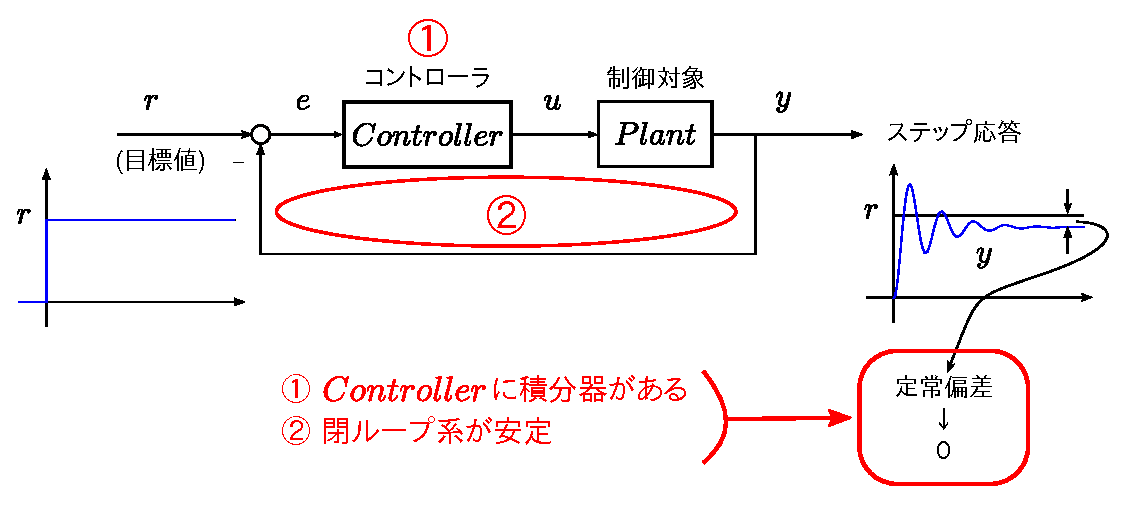
\includegraphics[width=0.9\linewidth]{sfigure/stdError.eps}
  \caption{古典制御理論におけるサーボ系}
  \label{fig_servo0}
 \end{center}
\end{figure}
\end{frame}


%%%%%%%%%%%%%%%%%%%%%%%%%%%%%%%%%%%%%%%%%%%%%%%%%%%%%%%%%%%%%%
\begin{frame}[t]
\frametitle{1.9 状態フィードバック (サーボ系)}
%-------------------------------------------------------------
ここではシステム(\ref{state_eq})(\ref{output_eq})において$D=0$とした以
下の系を考える．
\begin{align}
 \frac{dx}{dt} &= A x + B u \label{st_proper_state_eq} \\
 y             &= C x \label{st_proper_output_eq}
\end{align}
さらに$y \in \mathbb{R}^m$であり，入力と出力の次数が等しいとする．

追従誤差を$e=r-y$として次式で積分器を導入する．
\begin{equation}
 \eta = \int_0^t e \ d \tau
\end{equation}
両辺を$t$ で微分すると，
\begin{equation}
 \frac{d \eta}{dt} = e= r - y = r - Cx
\end{equation}
をとなり，積分器を状態方程式（微分方程式）で表すことができる．
\end{frame}


%%%%%%%%%%%%%%%%%%%%%%%%%%%%%%%%%%%%%%%%%%%%%%%%%%%%%%%%%%%%%%
\begin{frame}[t]
\frametitle{1.9 状態フィードバック (サーボ系)}              %%
%-------------------------------------------------------------
\addtocounter{equation}{-1}
$D=0$ のシステム
\begin{align}
 \frac{dx}{dt} &= A x + B u \tag{\ref{st_proper_state_eq}} \\
 y             &= C x \tag{\ref{st_proper_output_eq}}
\end{align}
積分器
\begin{align}
 \frac{d \eta}{dt} &= r - Cx
\end{align}

これらを
を合わしたFig.~\ref{fig_servo1}のシステム(拡大系)は
\begin{align}
 \frac{d}{dt}
  \left(\begin{array}{c}
         x \\
   \eta
  \end{array}\right)
  &=
  \left(\begin{array}{cc}
         A  & 0 \\
   -C & 0
  \end{array}\right)
  \left(\begin{array}{c}
         x \\
   \eta
  \end{array}\right)
  +
  \left(\begin{array}{c}
         B \\
   0
  \end{array}\right)
  u +
  \left(\begin{array}{c}
         0 \\
   I
  \end{array}\right)
  r \\
 y &=
  \left(\begin{array}{cc}
         C & 0
  \end{array}\right)
  \left(\begin{array}{c}
         x \\
   \eta
  \end{array}\right)
\end{align}
となる．
\end{frame}


%%%%%%%%%%%%%%%%%%%%%%%%%%%%%%%%%%%%%%%%%%%%%%%%%%%%%%%%%%%%%%
\begin{frame}[t]
\frametitle{1.9 状態フィードバック (サーボ系)}
%-------------------------------------------------------------
\begin{figure}[t]
 \begin{center}
  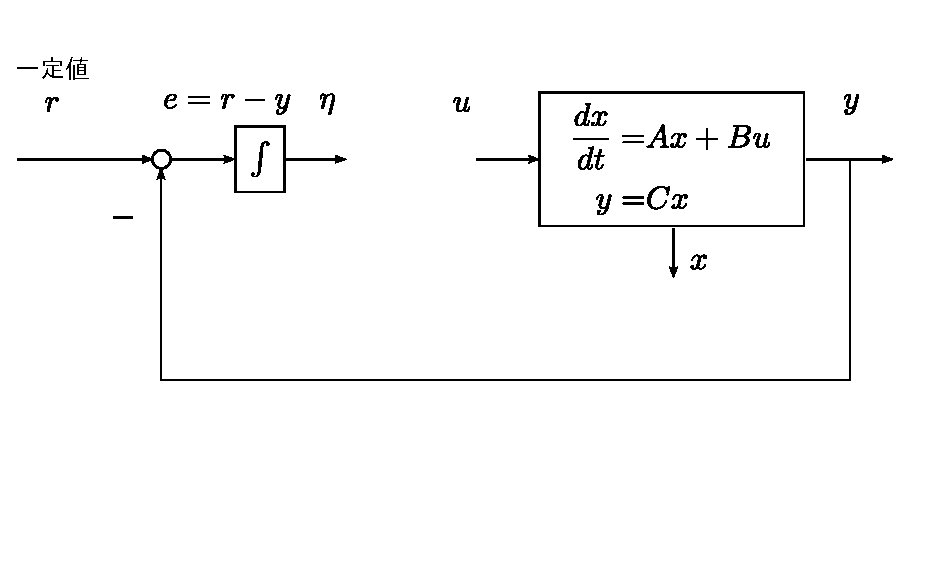
\includegraphics[width=0.7\linewidth]{sfigure/servo1.eps}
  \caption{積分器を含む拡大系}
  \label{fig_servo1}
 \end{center}
\end{figure}
\end{frame}


%%%%%%%%%%%%%%%%%%%%%%%%%%%%%%%%%%%%%%%%%%%%%%%%%%%%%%%%%%%%%%
\begin{frame}[t]
\frametitle{1.9 状態フィードバック (サーボ系)}
%-------------------------------------------------------------
このシステムは$(A,B)$可制御かつ
\begin{equation}
   \rank \left(\begin{array}{cc}
          A & B \\
    C & 0
         \end{array}\right)
   = n + m
\end{equation}
のとき安定化できることが知られている．
\end{frame}



%%%%%%%%%%%%%%%%%%%%%%%%%%%%%%%%%%%%%%%%%%%%%%%%%%%%%%%%%%%%%%
\begin{frame}[t]
\frametitle{1.9 状態フィードバック (サーボ系)}
%-------------------------------------------------------------
\begin{figure}[b]
 \begin{center}
  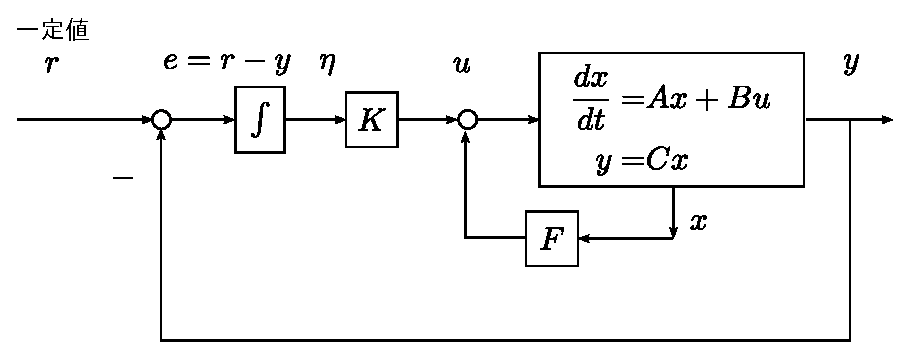
\includegraphics[width=0.7\linewidth]{sfigure/servo2.eps}
  \caption{サーボ系}
  \label{fig_servo2}
 \end{center}
\end{figure}
この拡大システムを安定化させる状態フィードバックは極配置法や最適制御法で求めることができる．
状態フィードバックは
\begin{equation}
 u = \left(\begin{array}{cc}
            F & K
     \end{array}\right)
 \left(\begin{array}{c}
        x \\
  \eta
       \end{array}\right)
   = F x + K \eta
\end{equation}
であり，ブロック線図で表せばFig.~\ref{fig_servo2}となる．このシステムは (1)~コントローラに積分器を含み，(2)~閉ループ系が安定，であることから，ステップ目標値（一定目標値）$r$に対して出力$y$が定常偏差を持たずに追従するサーボ系となる．
\end{frame}


%%%%%%%%%%%%%%%%%%%%%%%%%%%%%%%%%%%%%%%%%%%%%%%%%%%%%%%%%%%%%%
\begin{frame}[t]
\frametitle{1.9 状態フィードバック (サーボ系)}
%-------------------------------------------------------------
定常偏差が$0$となる理由を考察する．
閉ループ系は
\begin{align}
 \frac{d}{dt}
  \left(\begin{array}{c}
         x \\
   \eta
  \end{array}\right)
  &=
  \left(\begin{array}{cc}
         A + B F & B K \\
   - C     & 0
  \end{array}\right)
  \left(\begin{array}{c}
         x \\
   \eta
  \end{array}\right)
  +
  \left(\begin{array}{c}
         0 \\
   I
  \end{array}\right)
  r \\
 y &=
  \left(\begin{array}{cc}
         C & 0
  \end{array}\right)
  \left(\begin{array}{c}
         x \\
   \eta
  \end{array}\right)
\end{align}
となる．\\
システムは安定であるから$r$を一定値とすると，$t \rightarrow \infty$で\\
\hspace*{1cm} 状態$x$はある値 $x_{\infty}$，\\
\hspace*{1cm} 積分器の状態$\eta$はある値 $\eta_{\infty}$\\
にそれぞれ収束する．\\
（閉ループ系が安定であるから，一定目標値$r$が入ったとしても，\\
システムが振動したり，発散しないことは容易に推測できる）
\end{frame}


%%%%%%%%%%%%%%%%%%%%%%%%%%%%%%%%%%%%%%%%%%%%%%%%%%%%%%%%%%%%%%
\begin{frame}[t]
\frametitle{1.9 状態フィードバック (サーボ系)}
%-------------------------------------------------------------
定常偏差が$0$となる理由を考察する．
閉ループ系は
\addtocounter{equation}{-2}
\begin{align}
 \frac{d}{dt}
  \left(\begin{array}{c}
         x \\
   \eta
  \end{array}\right)
  &=
  \left(\begin{array}{cc}
         A + B F & B K \\
   - C     & 0
  \end{array}\right)
  \left(\begin{array}{c}
         x \\
   \eta
  \end{array}\right)
  +
  \left(\begin{array}{c}
         0 \\
   I
  \end{array}\right)
  r \\
 y &=
  \left(\begin{array}{cc}
         C & 0
  \end{array}\right)
  \left(\begin{array}{c}
         x \\
   \eta
  \end{array}\right)
\end{align}

よって出力$y$も$y_{\infty} = C x_{\infty}$に収束する．$t
\rightarrow \infty $において$\eta$が収束することから
\begin{equation}
 \lim_{t \rightarrow \infty} \frac{d \eta}{dt} = 0
\end{equation}
でなければならない．これは
\begin{equation}
 \lim_{t \rightarrow \infty} \frac{d \eta}{dt}
  = r - y_{\infty} = 0
\end{equation}
であることを示している．よって
\begin{equation}
   \lim_{t \rightarrow \infty} y(t) = y_\infty= r
\end{equation}
つまり，定常偏差が零となる．
\end{frame}

%%%%%%%%%%%%%%%%%%%%%%%%%%%%%%%%%%%%%%%%%%%%%%%%%%%%%%%%%%%%%%
\begin{frame}[t]
\frametitle{1.9 状態フィードバック ＜演習＞サーボ系}
%-------------------------------------------------------------
次のシステムに対して，一定目標値$r$に対して定常偏差なく追従するコントローラを設計せよ．ただし，閉ループ系のすべての極を$-1$とせよ．
\begin{align*}
	\frac{dx}{dt} &= 1 \cdot x + 1 \cdot u, \hspace{0cm} &A=1,\  B=1
\\
	y &= 1 \cdot x , &C=1, \ D=0
\end{align*}
\end{frame}


%%%%%%%%%%%%%%%%%%%%%%%%%%%%%%%%%%%%%%%%%%%%%%%%%%%%%%%%%%%%%%
\begin{frame}[t]
\frametitle{1.9 状態フィードバック (内部モデル原理)}
%-------------------------------------------------------------
ここではステップ目標値に定常偏差なく追従する制御系を設計した．\\
\begin{itemize}
  \item ランプ目標値($r(t)=t$)に追従するためには一巡伝達関数が$\frac{1}{s^2}$\\
  \item 一定加速度目標値($r(t)=\frac{t^2}{2}$）に追従するためには一巡伝達関数が$\frac{1}{s^3}$
\end{itemize}
を含んでいればよいことが分かっている．
これは\\
\begin{itemize}
  \item ステップ目標値($r(t)=1$)のラプラス変換は$\frac{1}{s}$
  \item ランプ目標値は$\frac{1}{s^2}$
  \item 一定加速度目標値は$\frac{1}{s^3}$
\end{itemize}
であることを考えれば，つぎのことが知られている．
\begin{block}{\bf 内部モデル原理(internal model principle)}
目標値のラプラス変換と同じ伝達関数を一巡伝達関数に含んでいれば定常偏差なく追従できる．
\end{block}
例えば同様に$r(t)= \sin \omega t$に追従するためには$\sin \omega t$のラプラス変換である$\frac{\omega}{s^2 + \omega^2}$を一巡伝達関数が含んでいれば定常偏差なく追従できることが知られている．
\end{frame}


%%%%%%%%%%%%%%%%%%%%%%%%%%%%%%%%%%%%%%%%%%%%%%%%%%%%%%%%%%%%%%
\begin{frame}[t]
\frametitle{1.9 状態フィードバック (内部モデル原理)}
%-------------------------------------------------------------
\vspace{-3mm}
それぞれの伝達関数の状態方程式表現は
\begin{align}
\frac{1}{s^2}: & \hspace*{3mm}
 \frac{d}{dt}
  \left(\begin{array}{c}
         \eta_1 \\
   \eta_2
  \end{array}\right)
  =
  \left(\begin{array}{cc}
         0 & 1 \\
   0 & 0
  \end{array}\right)
  \left(\begin{array}{c}
         \eta_1 \\
   \eta_2
  \end{array}\right)
  +
  \left(\begin{array}{c}
         0 \\
   1
  \end{array}\right)
  u
  \notag \\ & \hspace*{18mm}
  y =
  \left(\begin{array}{cc}
         1 & 0
  \end{array}\right)
  \left(\begin{array}{c}
         \eta_1 \\
   \eta_2
  \end{array}\right)
\\
\frac{1}{s^3}: &  \hspace*{3mm}
 \frac{d}{dt}
  \left(\begin{array}{c}
         \eta_1 \\
         \eta_2 \\
   \eta_3
  \end{array}\right)
  =
  \left(\begin{array}{ccc}
         0 & 1 & 0\\
   0 & 0 & 1\\
   0 & 0 & 0
  \end{array}\right)
  \left(\begin{array}{c}
         \eta_1 \\
         \eta_2 \\
   \eta_3
  \end{array}\right)
  +
  \left(\begin{array}{c}
         0 \\
         0 \\
   1
  \end{array}\right)
  u
  \notag \\ & \hspace*{18mm}
  y =
  \left(\begin{array}{ccc}
         1 & 0 & 0
  \end{array}\right)
  \left(\begin{array}{c}
         \eta_1 \\
         \eta_2 \\
   \eta_3
  \end{array}\right)
\\
\frac{\omega}{s^2+\omega^2}: & \hspace*{3mm}
 \frac{d}{dt}
  \left(\begin{array}{c}
         \eta_1 \\
   \eta_2
  \end{array}\right)
  =
  \left(\begin{array}{cc}
         0 & \omega \\
   -\omega & 0
  \end{array}\right)
  \left(\begin{array}{c}
         \eta_1 \\
   \eta_2
  \end{array}\right)
  +
  \left(\begin{array}{c}
         0 \\
   1
  \end{array}\right)
  u
  \notag \\ & \hspace*{18mm}
  y =
  \left(\begin{array}{cc}
         1 & 0
  \end{array}\right)
  \left(\begin{array}{c}
         \eta_1 \\
   \eta_2
  \end{array}\right)
\end{align}
であることから，これらの状態方程式部分を用いて拡大系を構成し，安定化すればこれらの目標値に対して定常偏差なく追従する制御系が設計できる
.
\end{frame}


%%%%%%%%%%%%%%%%%%%%%%%%%%%%%%%%%%%%%%%%%%%%%%%%%%%%%%%%%%%%%%
\begin{frame}[t]
\frametitle{1.9 状態フィードバック (拡大系の可制御性の例題)}
%-------------------------------------------------------------
ここでは拡大系が可制御となるための条件
\begin{equation}
   \rank \left(\begin{array}{cc}
          A & B \\
    C & 0
         \end{array}\right)
   = n + m
\end{equation}
について考える．\\

\noindent
\underline{拡大系が可制御となる例}

次のシステムを考える．
\begin{align}
 \frac{d}{dt}
 \left(
 \begin{array}{c}
  x_1 \\
  x_2
 \end{array}
 \right) &=
 \left(
 \begin{array}{cc}
  0 & 1 \\
  1 & 2 \\
 \end{array}
 \right)
 \left(
 \begin{array}{c}
  x_1 \\
  x_2
 \end{array}
 \right) +
 \left(
 \begin{array}{c}
  0 \\
  1
 \end{array}
 \right) u \\
 y &=
 \left(
 \begin{array}{cc}
  1 & 0
 \end{array}
 \right)
 \left(
 \begin{array}{c}
  x_1 \\
  x_2
 \end{array}
 \right)
\end{align}
\end{frame}


%%%%%%%%%%%%%%%%%%%%%%%%%%%%%%%%%%%%%%%%%%%%%%%%%%%%%%%%%%%%%%
\begin{frame}[t]
\frametitle{1.9 状態フィードバック (拡大系の可制御性の例題)}
%-------------------------------------------------------------
このシステムに積分器
\begin{align}
 \frac{d\eta}{dt} &= r - y \\
 &= r - Cx \\
 &= r - \left(\begin{array}{cc}1 & 0\end{array}\right)x
\end{align}
を導入して拡大系を構成すると，
\begin{align}
 \frac{d}{dt}
 \left(
 \begin{array}{c}
  x_1 \\
  x_2 \\
  \eta
 \end{array}
 \right) &=
 \left(
 \begin{array}{ccc}
  0 & 1 & 0 \\
  1 & 2 & 0 \\
  -1 & 0 & 0 \\
 \end{array}
 \right)
 \left(
 \begin{array}{c}
  x_1 \\
  x_2 \\
  \eta
 \end{array}
 \right) +
 \left(
 \begin{array}{c}
  0 \\
  1 \\
  0
 \end{array}
 \right) u +
 \left(
 \begin{array}{c}
  0 \\
  0 \\
  1
 \end{array}
 \right) r \\
 y &=
 \left(
 \begin{array}{ccc}
  1 & 0 & 0
 \end{array}
 \right)
 \left(
 \begin{array}{c}
  x_1 \\
  x_2 \\
  \eta
 \end{array}
 \right)
\end{align}
となり，
\end{frame}


%%%%%%%%%%%%%%%%%%%%%%%%%%%%%%%%%%%%%%%%%%%%%%%%%%%%%%%%%%%%%%
\begin{frame}[t]
\frametitle{1.9 状態フィードバック (拡大系の可制御性の例題)}
%-------------------------------------------------------------
\vspace*{-5mm}

\begin{gather}
 \rank
 \left(
 \begin{array}{cc}
  B & AB
 \end{array}
 \right) =
 \rank
 \left(
 \begin{array}{cc}
  0 & 1 \\
  1 & 2
 \end{array}
 \right) = 2 \\
 \rank
 \left(
 \begin{array}{cc}
  A & B \\
  C & 0
 \end{array}
 \right) =
 \rank
 \left(
 \begin{array}{ccc}
  0 & 1 & 0 \\
  1 & 2 & 1 \\
  1 & 0 & 0
 \end{array}
 \right) =
 3(= 2 + 1)
\end{gather}
であるので，この場合安定化可能なはずである．
実際，拡大系の可制御性行列は

\begin{align}
 V &=
 \left\{
 \begin{array}{ccc}
 \left(
 \begin{array}{c}
  0 \\
  1 \\
  0
 \end{array}
 \right) &
 \left(
 \begin{array}{ccc}
  0 & 1 & 0 \\
  1 & 2 & 0 \\
  -1 & 0 & 0 \\
 \end{array}
 \right)
 \left(
 \begin{array}{c}
  0 \\
  1 \\
  0
 \end{array}
 \right) &
 \left(
 \begin{array}{ccc}
  0 & 1 & 0 \\
  1 & 2 & 0 \\
  -1 & 0 & 0 \\
 \end{array}
 \right)^2
 \left(
 \begin{array}{c}
  0 \\
  1 \\
  0
 \end{array}
 \right)
 \end{array}
 \right\} \notag\\&=
 \left(
 \begin{array}{ccc}
  0 & 1 & 2 \\
  1 & 2 & 5 \\
  0 & 0 & -1 \\
 \end{array}
 \right)\notag
\end{align}
となり，$\rank V = 3$であるので拡大系は可制御である．
\end{frame}


%%%%%%%%%%%%%%%%%%%%%%%%%%%%%%%%%%%%%%%%%%%%%%%%%%%%%%%%%%%%%%
\begin{frame}[t]
\frametitle{1.9 状態フィードバック (拡大系が不可制御となる例)}
%-------------------------------------------------------------
制御対象が可制御であるにもかかわらず，拡大系が不可制御となる例を示す．
\begin{align}
 \frac{d}{dt}
 \left(
 \begin{array}{c}
  x_1 \\
  x_2
 \end{array}
 \right) &=
 \left(
 \begin{array}{cc}
  0 & 1 \\
  1 & 2 \\
 \end{array}
 \right)
 \left(
 \begin{array}{c}
  x_1 \\
  x_2
 \end{array}
 \right) +
 \left(
 \begin{array}{c}
  0 \\
  1
 \end{array}
 \right) u \\
 y &=
 \left(
 \begin{array}{cc}
  0 & 1
 \end{array}
 \right)
 \left(
 \begin{array}{c}
  x_1 \\
  x_2
 \end{array}
 \right)
\end{align}
で表されるシステムに積分器
\begin{align}
 \frac{d\eta}{dt} &= r - y \\
 &= r - Cx \\
 &= r - \left(\begin{array}{cc}0 & 1\end{array}\right)x
\end{align}
を導入して拡大系を構成すると，
\end{frame}


%%%%%%%%%%%%%%%%%%%%%%%%%%%%%%%%%%%%%%%%%%%%%%%%%%%%%%%%%%%%%%
\begin{frame}[t]
\frametitle{1.9 状態フィードバック (拡大系が不可制御となる例)}
%-------------------------------------------------------------
\vspace*{-5mm}

\begin{align}
 \frac{d}{dt}
 \left(
 \begin{array}{c}
  x_1 \\
  x_2 \\
  \eta
 \end{array}
 \right) &=
 \left(
 \begin{array}{ccc}
  0 & 1 & 0 \\
  1 & 2 & 0 \\
  0 & -1 & 0 \\
 \end{array}
 \right)
 \left(
 \begin{array}{c}
  x_1 \\
  x_2 \\
  \eta
 \end{array}
 \right) +
 \left(
 \begin{array}{c}
  0 \\
  1 \\
  0
 \end{array}
 \right) u +
 \left(
 \begin{array}{c}
  0 \\
  0 \\
  1
 \end{array}
 \right) r \\
 y &=
 \left(
 \begin{array}{ccc}
  0 & 1 & 0
 \end{array}
 \right)
 \left(
 \begin{array}{c}
  x_1 \\
  x_2 \\
  \eta
 \end{array}
 \right)
\end{align}
となる．元のシステムは
\begin{gather}
 \rank
 \left(
 \begin{array}{cc}
  B & AB
 \end{array}
 \right) =
 \rank
 \left(
 \begin{array}{cc}
  0 & 1 \\
  1 & 2
 \end{array}
 \right) = 2 \\
\end{gather}
と可制御であるが，
\begin{gather}
 \rank
 \left(
 \begin{array}{cc}
  A & B \\
  C & 0
 \end{array}
 \right) =
 \rank
 \left(
 \begin{array}{ccc}
  0 & 1 & 0 \\
  1 & 2 & 1 \\
  0 & 1 & 0
 \end{array}
 \right) =
 2 < 3(= 2 + 1)
\end{gather}
であるので，この場合，拡大系の安定化は不可能となる．
\end{frame}


%%%%%%%%%%%%%%%%%%%%%%%%%%%%%%%%%%%%%%%%%%%%%%%%%%%%%%%%%%%%%%
\begin{frame}[t]
\frametitle{1.9 状態フィードバック (拡大系が不可制御となる例)}
%-------------------------------------------------------------
実際，拡大系の可制御性行列は
\begin{align}
 V &=
 \left\{
 \begin{array}{ccc}
 \left(
 \begin{array}{c}
  0 \\
  1 \\
  0
 \end{array}
 \right) &
 \left(
 \begin{array}{ccc}
  0 & 1 & 0 \\
  1 & 2 & 0 \\
  0 & -1 & 0 \\
 \end{array}
 \right)
 \left(
 \begin{array}{c}
  0 \\
  1 \\
  0
 \end{array}
 \right) &
 \left(
 \begin{array}{ccc}
  0 & 1 & 0 \\
  1 & 2 & 0 \\
  0 & -1 & 0 \\
 \end{array}
 \right)^2
 \left(
 \begin{array}{c}
  0 \\
  1 \\
  0
 \end{array}
 \right)
 \end{array}
 \right\} \notag\\ &=
 \left(
 \begin{array}{ccc}
  0 & 1 & 2 \\
  1 & 2 & 5 \\
  0 & -1 & -2 \\
 \end{array}
 \right)\notag
\end{align}
となり，$\rank V = 2<3$であるので拡大系は不可制御である．\\
\end{frame}


%%%%%%%%%%%%%%%%%%%%%%%%%%%%%%%%%%%%%%%%%%%%%%%%%%%%%%%%%%%%%%
\begin{frame}[t]
\frametitle{1.9 状態フィードバック (拡大系が不可制御となる例)}
%-------------------------------------------------------------
この例は次のように解釈できる．制御対象の伝達関数は
\[
 G(s) = C(sI-A)^{-1}B = \frac{s}{s^2-2s-1}
\]
となり，$s=0$に零点を持っている（原点に零点を持っている）．\\
サーボ系を構成するためには制御対象と積分器$1/s$を直列結合する必要があるが，
積分器の$s=0$ の極（原点極）と制御対象の原点零点が不安定な極零相殺を起こすためにサーボ系が構成できない．
\end{frame}


%%%%%%%%%%%%%%%%%%%%%%%%%%%%%%%%%%%%%%%%%%%%%%%%%%%%%%%%%%%%%%
\begin{frame}[t]
\frametitle{1.10 オブザーバと出力フィードバック (オブザーバ)}
%-------------------------------------------------------------
これまではシステムを状態フィードバックにより安定化することを考えてきた．\\
しかし，Fig.~\ref{fig_obs1}に示すように，状態$x$は内部状態であり，$x$を直接を直接知ることはできない．そこで\Blue{\bf オブザーバ（状態観測器）(state observer)}を用いて，直接入手可能な入力$u$と出力$y$から状態$x$を推定する方法について考える．

本節ではシステムにおいて$D=0$とした以下の系を考える．
\begin{align}
 \frac{dx}{dt} &= A x + B u \label{st_proper_state_eq_2} \\
 y             &= C x \label{st_proper_output_eq_2}
\end{align}
\begin{figure}
 \begin{center}
  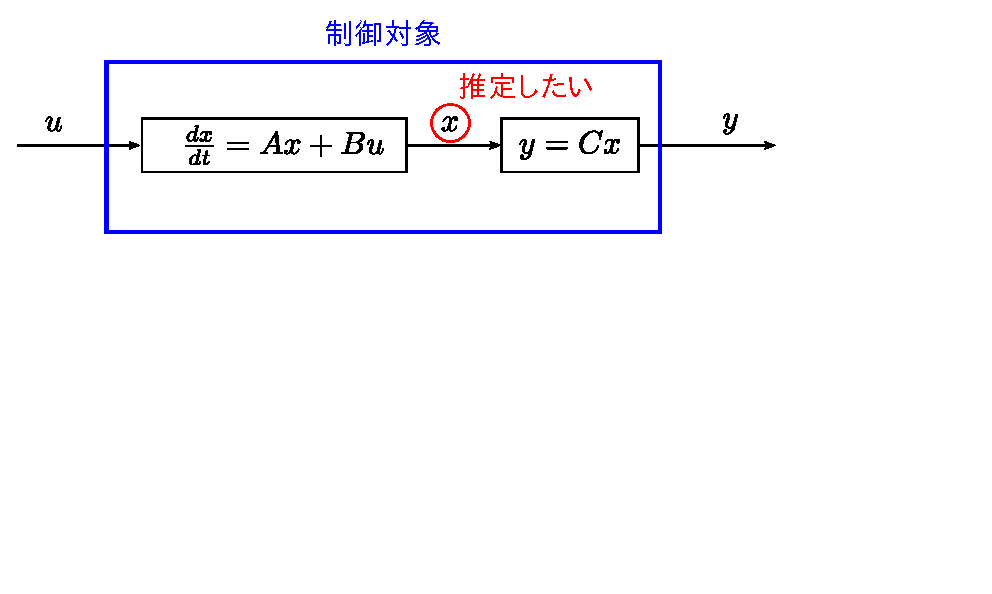
\includegraphics[width=1.0\linewidth]{sfigure/observer2.eps}
  \caption{制御対象}
  \label{fig_obs1}
 \end{center}
\end{figure}
\end{frame}


%%%%%%%%%%%%%%%%%%%%%%%%%%%%%%%%%%%%%%%%%%%%%%%%%%%%%%%%%%%%%%
\begin{frame}[t]
\frametitle{1.10 オブザーバと出力フィードバック \\
(同一次元オブザーバ)}
%-------------------------------------------------------------
\vspace*{-5mm}

\begin{figure}[H]
 \begin{center}
 \only<1>{
  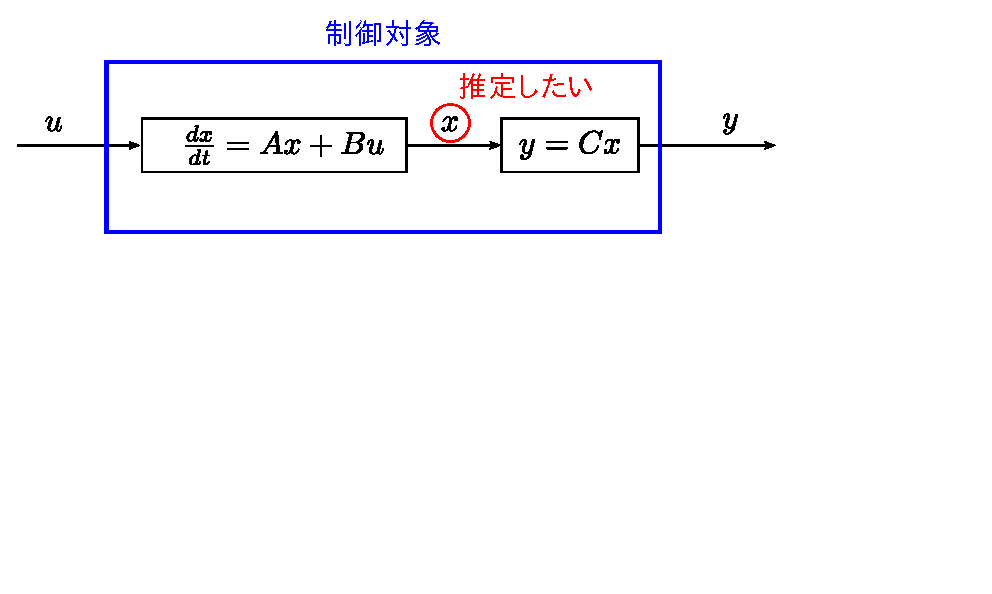
\includegraphics[width=0.7\linewidth]{sfigure/observer2.eps}
 }
 \only<2,3>{
  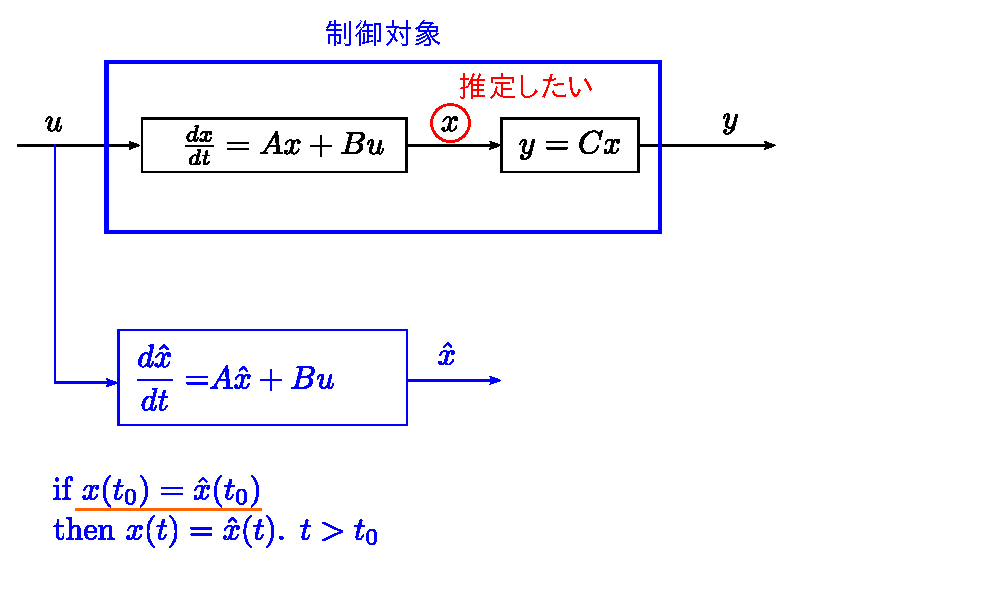
\includegraphics[width=0.7\linewidth]{sfigure/observer3.eps}
 }
 \only<4,5>{
  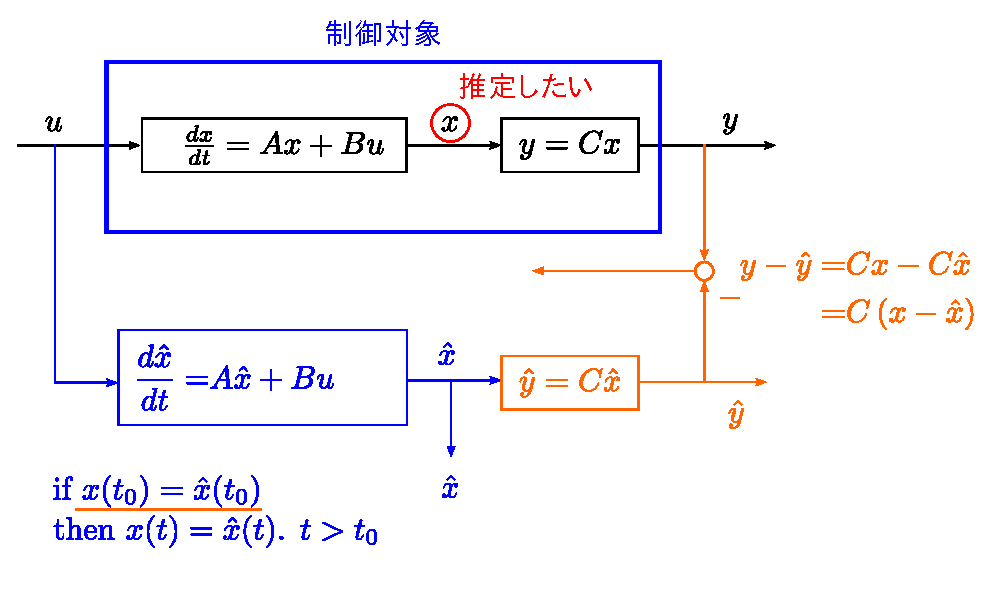
\includegraphics[width=0.7\linewidth]{sfigure/observer4.eps}
 }
 \only<6,7>{
  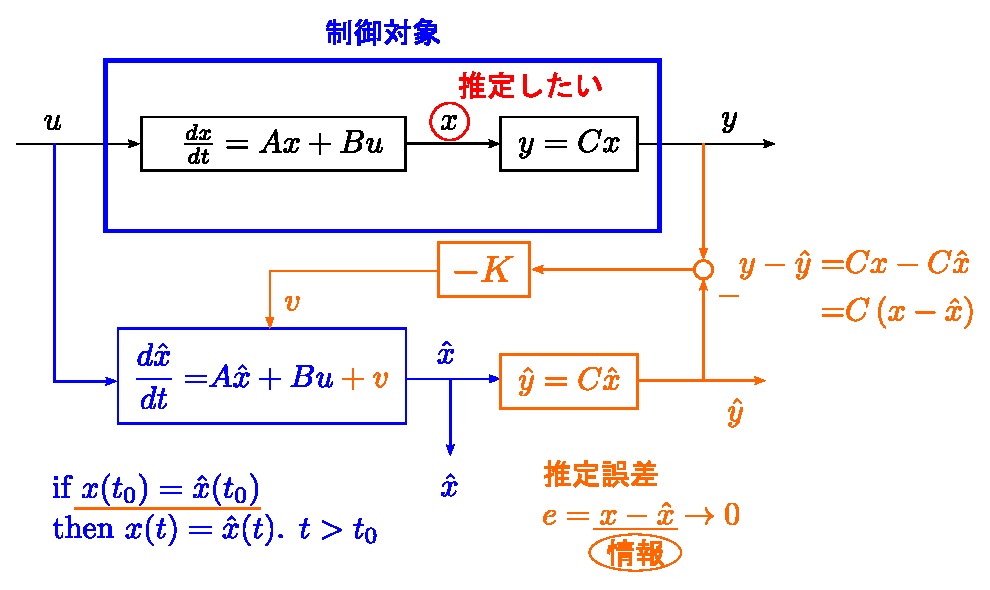
\includegraphics[width=0.7\linewidth]{sfigure/observer5.eps}
 }
 \end{center}
\end{figure}
\vspace*{-5mm}

\only<1>{
  内部に隠れた$x$を推定する方法を考えよう．
}
\only<2>{
  青い部分のように，制御対象のモデル
  \begin{equation}
   \frac{d \hat{x}}{dt} = A \hat{x} + B u \tag{1.201}
  \end{equation}
  を用いて，$x$の推定値$\hat{x}$を求めることを考えよう．
}
\only<3>{
計算機内でこのモデルを計算する（シミュレーションする）ことにより，\\
$x$の推定値$\hat{x}$を求めるという戦略である．\\
制御対象の初期値$x(0)$と推定器（モデル）の初期値$\hat{x}(0)$が等しければ，\\
$x(t)=\hat{x}(t)$となり，状態の推定が可能となる．\\
しかし，このままでは$x(0)$と$\hat{x}(0)$が等しくない場合には推定できない．
}
\only<4>{
推定誤差$e=x-\hat{x}$を用いて$\hat{x}$を修正することを考える．\\
しかし，$x$は直接観測することができないため出力$y$を用いる．\\
$\hat{y}=C\hat{x}$と定義すれば，これは状態が推定値$\hat{x}$であったとしたときの推定出力と考えることができる．
}
\only<5>{
この推定出力と出力の差は
\begin{equation}
  y-\hat{y}=Cx-C\hat{x}=C(x-\hat{x}) \tag{1.203}
\end{equation}
となり，$e=x-\hat{x}$の情報を持っている．
}
\only<6>{
これをゲイン$K$を介して$v$に入力することにより，
$\hat{x}$を修正する．
\begin{equation}
 \frac{d \hat{x}}{dt} = A \hat{x} + B u + v \tag{1.202}
\end{equation}
}
\only<7>{
  このように考えて構成されたのが次のシステムである．
  \begin{equation}
   \frac{d \hat{x}}{dt} = A \hat{x} + B u - K (y - C \hat{x})
   \tag{1.204} \label{obs_org}
  \end{equation}
}

\end{frame}


%%%%%%%%%%%%%%%%%%%%%%%%%%%%%%%%%%%%%%%%%%%%%%%%%%%%%%%%%%%%%%
\begin{frame}[t]
\frametitle{1.10 オブザーバと出力フィードバック \\
(同一次元オブザーバ)}
%-------------------------------------------------------------
システム
\begin{align}
 \frac{dx}{dt} &= A x + B u \tag{\ref{st_proper_state_eq_2}} \\
 y             &= C x \tag{\ref{st_proper_output_eq_2}}
\end{align}
状態の推定器
\begin{align}
 \frac{d \hat{x}}{dt} &= A \hat{x} + B u - K (y - C \hat{x})
 \tag{1.204} \label{obs_org}
\end{align}
\addtocounter{equation}{4}
いまシステム(\ref{st_proper_state_eq_2})の状態$x$とシステム
(\ref{obs_org})の状態$\hat{x} $の差を
\begin{equation}
 e \defeq x - \hat{x}
\end{equation}
とすれば
\begin{align}
\frac{de}{dt} &= \frac{dx}{dt} - \frac{d \hat{x}}{dt} 
  = A x + B u - A \hat{x} - B u + K ( C x - C \hat{x}) \nonumber \\
 &= A (x - \hat{x}) + K ( C x - C \hat{x}) \nonumber \\
 &= (A + KC) e
\end{align}
\end{frame}


%%%%%%%%%%%%%%%%%%%%%%%%%%%%%%%%%%%%%%%%%%%%%%%%%%%%%%%%%%%%%%
\begin{frame}[t]
\frametitle{1.10 オブザーバと出力フィードバック \\
(同一次元オブザーバ)}
%-------------------------------------------------------------

推定誤差($e = x - \hat{x}$)の微分方程式
\begin{align}
\frac{de}{dt} = (A + KC) e \tag{1.206}
\end{align}



$(A+KC)$が安定になるように$K$を選べば，入力や初期値$\hat{x}(0)$に
よらず$e \rightarrow 0$, つまり$\hat{x} \rightarrow x$となることが分かる．
このようにシステム
\begin{align}
 \frac{d \hat{x}}{dt} &= A \hat{x} + B u - K (y - C \hat{x})
 \tag{1.204} \label{obs_org}
\end{align}
を用いればシステム(\ref{st_proper_state_eq_2})の状態$x$を
知ることができる．\\
このようなシステムを\Blue{\bf オブザーバ(状態観測器)(observer)}と呼ぶ．\\
\Blue{\bf $(A + KC)$を安定にする$K$は$(C, A)$が可観測であるときに存在する．}
\end{frame}


%%%%%%%%%%%%%%%%%%%%%%%%%%%%%%%%%%%%%%%%%%%%%%%%%%%%%%%%%%%%%%
\begin{frame}[t]
\frametitle{1.10 オブザーバと出力フィードバック \\
(簡単なシステムのオブザーバゲインの求め方（例）)}
%-------------------------------------------------------------
システム
\begin{align}
 \frac{d}{dt}
 \left(
 \begin{array}{c}
  x_1 \\
  x_2
 \end{array}
 \right)
 &=
 \left(
 \begin{array}{cc}
  0 & -1 \\
  1 & 1
 \end{array}
 \right)
 \left(
 \begin{array}{c}
  x_1 \\
  x_2
 \end{array}
 \right) +
 \left(
 \begin{array}{c}
  1 \\
  1
 \end{array}
 \right) u \\
 y &=
 \left(
 \begin{array}{cc}
  0 & 1
 \end{array}
 \right)
 \left(
 \begin{array}{c}
  x_1 \\
  x_2
 \end{array}
 \right)
\end{align}
に対して，同一次元オブザーバ
\begin{equation}
 \frac{d}{dt}
 \left(
 \begin{array}{c}
  \hat{x}_1 \\
  \hat{x}_2
 \end{array}
 \right)
 =
 \left(
 \begin{array}{cc}
  0 & -1 \\
  1 & 1
 \end{array}
 \right)
 \left(
 \begin{array}{c}
  \hat{x}_1 \\
  \hat{x}_2
 \end{array}
 \right) +
 \left(
 \begin{array}{c}
  1 \\
  1
 \end{array}
 \right) u -
 K\left\{y -
 \left(
 \begin{array}{cc}
  0 & 1
 \end{array}
 \right)
 \left(
 \begin{array}{c}
  \hat{x}_1 \\
  \hat{x}_2
 \end{array}
 \right)\right\}
\end{equation}
の極($(A+KC)$の極)が$-1, -2$となる$K$
\begin{align}
 K&=
 \left(
 \begin{array}{c}
  k_1 \\
  k_2
 \end{array}
 \right)
\end{align}
を求める．
\end{frame}


%%%%%%%%%%%%%%%%%%%%%%%%%%%%%%%%%%%%%%%%%%%%%%%%%%%%%%%%%%%%%%
\begin{frame}[t]
\frametitle{1.10 オブザーバと出力フィードバック \\
(簡単なシステムのオブザーバゲインの求め方（例）)}
%-------------------------------------------------------------
状態の推定誤差を$e = x - \hat{x}$すると，
\begin{align}
 \frac{de}{dt}
 &= (A+KC) e
 \nonumber \\
 &=
 \left\{
 \left(
 \begin{array}{cc}
  0 & -1 \\
  1 & 1
 \end{array}
 \right)
 + 
 \left( 
 \begin{array}{c}
  k_1 \\
  k_2
 \end{array}
 \right)
 \left(
 \begin{array}{cc}
  0 & 1
 \end{array}
 \right)
 \right\} e
\nonumber \\
 &=
 \left(
 \begin{array}{cc}
  0 & -1 +k_1\\
  1 & 1 + k_2
 \end{array}
 \right)  e
\end{align}
となる．この特性多項式は
\begin{align}
 \det (sI-(A+KC))
 &=\det 
  \left(
  \begin{array}{cc}
   s & 1 -k_1\\
   -1 & s-1 - k_2
  \end{array}
  \right)
 \nonumber \\
 &= s^2 + (-k_2 - 1)s + (-k_1 + 1)
\end{align}
\end{frame}


%%%%%%%%%%%%%%%%%%%%%%%%%%%%%%%%%%%%%%%%%%%%%%%%%%%%%%%%%%%%%%
\begin{frame}[t]
\frametitle{1.10 オブザーバと出力フィードバック \\
(簡単なシステムのオブザーバゲインの求め方（例）)}
%-------------------------------------------------------------
この特性多項式は$s^2 + (-k_2 - 1)s + (-k_1 + 1)$ と\\
極が$-1, -2$となる特性多項式$(s+1)(s+2) = s^2 + 3s + 2$の係数比較より\\
$k_1 = -1$, $k_2 = -4$となるので，求めるオブザーバのゲイン$K$は
\[
 K =
 \left(
 \begin{array}{c}
  -1 \\
  -4
 \end{array}
 \right)
\]
と求めることができる．
これを元の同一次元オブザーバに戻すとその状態方程式は
{\small
\begin{align}
 \frac{d}{dt}
 \left(
 \begin{array}{c}
  \hat{x}_1 \\
  \hat{x}_2
 \end{array}
 \right)
 =&
 \left(
 \begin{array}{cc}
  0 & -1 \\
  1 & 1
 \end{array}
 \right)
 \left(
 \begin{array}{c}
  \hat{x}_1 \\
  \hat{x}_2
 \end{array}
 \right) +
 \left(
 \begin{array}{c}
  1 \\
  1
 \end{array}
 \right) u -
  \left(
 \begin{array}{c}
  -1 \\
  -4
 \end{array}
 \right)
\left\{y -
 \left(
 \begin{array}{cc}
  0 & 1
 \end{array}
 \right)
 \left(
 \begin{array}{c}
  \hat{x}_1 \\
  \hat{x}_2
 \end{array}
 \right)\right\} \notag \\
=&
 \left(
 \begin{array}{cc}
  0 & -2 \\
  1 & -3
 \end{array}
 \right)
 \left(
 \begin{array}{c}
  \hat{x}_1 \\
  \hat{x}_2
 \end{array}
 \right) +
 \left(
 \begin{array}{c}
  1 \\
  1
 \end{array}
 \right) u -
  \left(
 \begin{array}{c}
  -1 \\
  -4
 \end{array}
 \right)
y
\end{align}
}
となる．

\end{frame}


%%%%%%%%%%%%%%%%%%%%%%%%%%%%%%%%%%%%%%%%%%%%%%%%%%%%%%%%%%%%%%
\begin{frame}[t]
\frametitle{1.10 オブザーバと出力フィードバック \\
(状態フィードバックの設計を応用)}
%-------------------------------------------------------------
オブザーバのゲイン$K$は状態フィードバックの設計法を応用して次のように求められる．次の状態方程式を考える．
\begin{equation}
 \frac{d \xi}{dt} = A^T \xi + C^T \eta
\label{obs_pole_tmp}
\end{equation}
この状態方程式を安定化させる状態フィードバック
\begin{equation}
 \eta =  K^T \xi
\end{equation}
を求めれば$A^T + C^T K^T$が安定になる．\\
\end{frame}


%%%%%%%%%%%%%%%%%%%%%%%%%%%%%%%%%%%%%%%%%%%%%%%%%%%%%%%%%%%%%%
\begin{frame}[t]
\frametitle{1.10 オブザーバと出力フィードバック \\
(状態フィードバックの設計を応用)}
%-------------------------------------------------------------
この$K$ を用いれば正方行列$M$と$M^T$の固有値が等しいことから
\\[5mm]
\hspace*{1cm}\Blue{\bf $A^T + C^T K^T$が安定 $\Longrightarrow$$ A + K C$も安定}\\[5mm]
後述するように，オブザーバを設計すべき元のシステム
\begin{align}
 \frac{dx}{dt} &= A x + B u \tag{\ref{st_proper_state_eq_2}} \\
 y             &= C x \tag{\ref{st_proper_output_eq_2}}
\end{align}
が可観測である時にシステム(\ref{obs_pole_tmp})は可制御になる．\\
\Blue{\bf 可観測なシステムはこの方法でオブザーバを設計できる}ことになる．
\end{frame}


%%%%%%%%%%%%%%%%%%%%%%%%%%%%%%%%%%%%%%%%%%%%%%%%%%%%%%%%%%%%%%
\begin{frame}[t]
\frametitle{1.10 オブザーバと出力フィードバック \\
(状態フィードバックの設計を応用)}
%-------------------------------------------------------------
$M$と$M^T$の固有値が等しいことは以下のように証明できる．行列$M$が
\begin{align}
   T^{-1}MT = \Lambda
\end{align}
と対角化できたとする．この時$\Lambda$の対角要素は$M$の固有値からなっている．\\
ここで$T^{-1}MT$を転置すると，
\begin{align}
   (T^{-1}MT)^T &=  \Lambda^T = \Lambda
\\
   (T^{-1}MT)^T &= T^T M^T T^{-T} = (T^{-T})^{-1} M^T T^{-T} = \bar{T}^{-1} M^T \bar{T}
\end{align}
ここで，$\bar{T} = T^{-T}$ とする($T^{-T} = (T^{-1})^T=(T^T)^{-1}$)．よって，
\begin{align}
   \bar{T}^{-1} M^T \bar{T} &=  \Lambda
\end{align}
となる．これは$M^{T}$が$\bar{T}$により$\Lambda$に対角化されることを意味している．よって，$\Lambda$の対角要素は$M^{T}$の固有値でもある．つまり，$M$と$M^{T}$
の固有値は等しい．
\end{frame}


%%%%%%%%%%%%%%%%%%%%%%%%%%%%%%%%%%%%%%%%%%%%%%%%%%%%%%%%%%%%%%
\begin{frame}[t]
\frametitle{1.10 オブザーバと出力フィードバック \\
(状態フィードバックの設計を応用)}
%-------------------------------------------------------------
つぎのシステムのオブザーバを設計するときに，$(A+KC)$の極（オブザーバの極）が$-1,-2$と
なるように$K$を定めるため，次のシステムの状態フィードバック（極配置）問題を考える．

\begin{align}
 \frac{d}{dt}
 \left(
 \begin{array}{c}
  x_1 \\
  x_2
 \end{array}
 \right)
 &=
 \left(
 \begin{array}{cc}
  0 & -1 \\
  1 & 1
 \end{array}
 \right)
 \left(
 \begin{array}{c}
  x_1 \\
  x_2
 \end{array}
 \right) +
 \left(
 \begin{array}{c}
  1 \\
  1
 \end{array}
 \right) u \\
 y &=
 \left(
 \begin{array}{cc}
  0 & 1
 \end{array}
 \right)
 \left(
 \begin{array}{c}
  x_1 \\
  x_2
 \end{array}
 \right)
\end{align}
\end{frame}


%%%%%%%%%%%%%%%%%%%%%%%%%%%%%%%%%%%%%%%%%%%%%%%%%%%%%%%%%%%%%%
\begin{frame}[t]
\frametitle{1.10 オブザーバと出力フィードバック \\
(状態フィードバックの設計を応用)}
%-------------------------------------------------------------
仮想フィードバック系
\begin{align}
 \frac{d\xi}{dt} &= A^T \xi + C^T \eta \nonumber \\
 &=
 \left(
 \begin{array}{cc}
  0 & 1 \\
  -1 & 1
 \end{array}
 \right) \xi +
 \left(
 \begin{array}{c}
  0 \\
  1
 \end{array}
 \right) \eta
\end{align}
いま$\eta = K^T \xi = (\begin{array}{cc}k_1 & k_2\end{array})\xi$とする
と，
\begin{equation}
 \frac{d\xi}{dt} =
 \left(
 \begin{array}{cc}
  0 & 1 \\
  -1+k_1 & 1 + k_2
 \end{array}
 \right) \xi
\end{equation}
となり，この特性多項式は$s^2 + (-k_2 - 1)s + (-k_1 + 1)$である．
一方，極が$-1, -2$となる特性多項式$(s+1)(s+2) = s^2 + 3s + 2$との
係数比較より$k_1 = -1$, $k_2 = -4$となるので，求めるオブザーバのゲイン$K$は
\[
 K =
 \left(
 \begin{array}{c}
  -1 \\
  -4
 \end{array}
 \right)
\]
と求めることができる．これは先の結果と一致する．
\end{frame}

%%%%%%%%%%%%%%%%%%%%%%%%%%%%%%%%%%%%%%%%%%%%%%%%%%%%%%%%%%%%%%
\begin{frame}[t]
\frametitle{1.10 オブザーバと出力フィードバック\\ ＜演習＞オブザーバ}
%-------------------------------------------------------------
次のシステムに対して，オブザーバを設計せよ．ただし，オブザーバの極は$-1,-2$とせよ．
\begin{align*}
	\frac{d}{dt}
	\left (
	\begin{array}{c}
	 x_1 \\ x_2 
	\end{array}
	\right )
	& = 
	\left (
	\begin{array}{cc}
	 0 & 2 \\
	 1 & -1
	\end{array}
	\right )
	\left (
	\begin{array}{c}
	 x_1 \\ x_2 
	\end{array}
	\right )
	+
	\left (
	\begin{array}{c}
	 1 \\ 1 
	\end{array}
	\right )
	u
\\
	y&=
	\left ( \begin{array}{cc}
		0 & 2 
	\end{array} \right )
	\left (	\begin{array}{c}
		x_1 \\ x_2 
	\end{array} \right )
\end{align*}
\end{frame}


%%%%%%%%%%%%%%%%%%%%%%%%%%%%%%%%%%%%%%%%%%%%%%%%%%%%%%%%%%%%%%
\begin{frame}[t]
\frametitle{1.10 オブザーバと出力フィードバック \\
(オブザーバによる状態フィードバック系の安定性)}
%-------------------------------------------------------------
システム
\begin{align}
 \frac{dx}{dt} &= A x + B u \\
 y             &= C x
\end{align}
を安定化する状態フィードバックが
\begin{equation}
 u = F x
\end{equation}
で与えられているとする．
また，同一次元オブザーバが
\begin{equation}
 \frac{d \hat{x}}{dt} = A \hat{x} + B u - K (y - C \hat{x})
  \label{eq:obs}
\end{equation}
で与えられているとき，状態$x$を推定値$\hat{x}$で置き換えたフィードバック
則
\begin{equation}
 u = F \hat{x}
\end{equation}
を用いたときのシステムの安定性について考える．\\
ただし，$A + BF$が安定となるように$F$は選ばれ，
$A + KC$が安定となるように$K$が選ばれていると仮定する．
\end{frame}


%%%%%%%%%%%%%%%%%%%%%%%%%%%%%%%%%%%%%%%%%%%%%%%%%%%%%%%%%%%%%%
\begin{frame}[t]
\frametitle{1.10 オブザーバと出力フィードバック \\
(オブザーバによる状態フィードバック系の安定性)}
%-------------------------------------------------------------
\begin{figure}[htbp]
 \begin{center}
  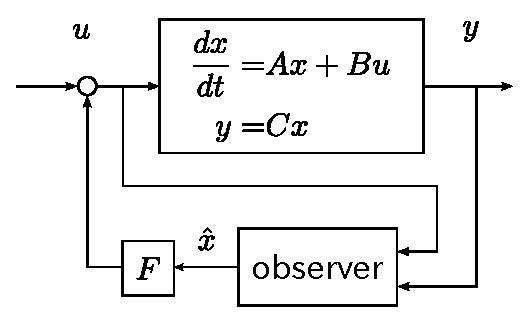
\includegraphics[width=0.6\linewidth]{sfigure/observer_simple.eps}
  \caption{オブザーバを用いたフィードバック系}
  \label{fig_obs_feedback}
 \end{center}
\end{figure}
結論から言えば，このオブザーバを用いた閉ループ系の極は状態フィードバックを設計したときの極とオブザーバの極と一致するため，
\Blue{両者を安定に設計すれば閉ループ系が必ず安定}となる．
これは次のように証明できる．

\end{frame}


%%%%%%%%%%%%%%%%%%%%%%%%%%%%%%%%%%%%%%%%%%%%%%%%%%%%%%%%%%%%%%
\begin{frame}[t]
\frametitle{1.10 オブザーバと出力フィードバック \\
(オブザーバによる状態フィードバック系の安定性)}
%-------------------------------------------------------------
まず，システムとオブザーバを合わせたシステム(併合系)は
\begin{equation}
 \frac{d}{dt}
  \left(\begin{array}{c}
         x \\
   \hat{x}
  \end{array}\right)
  =
  \left(\begin{array}{cc}
         A & 0 \\
   -KC & A+KC
  \end{array}\right)
  \left(\begin{array}{c}
         x \\
   \hat{x}
  \end{array}\right)
  +
  \left(\begin{array}{c}
         B \\
   B
  \end{array}\right)
  u
  \label{eq:hoge}
\end{equation}
となる．
ここで，次のような座標変換を考える．
\begin{equation}
 \left(\begin{array}{c}
         x \\
   \hat{x}
       \end{array}\right)
 =
 \left(\begin{array}{cc}
        I & 0 \\
  I & -I
       \end{array}\right)
 \left(\begin{array}{c}
         x \\
   x - \hat{x}
       \end{array}\right)
 \defeq T
 \left(\begin{array}{c}
         x \\
   e
       \end{array}\right)
\end{equation}
\end{frame}


%%%%%%%%%%%%%%%%%%%%%%%%%%%%%%%%%%%%%%%%%%%%%%%%%%%%%%%%%%%%%%
\begin{frame}[t]
\frametitle{1.10 オブザーバと出力フィードバック \\
(オブザーバによる状態フィードバック系の安定性)}
%-------------------------------------------------------------
座標変換によって得られる状態方程式は
\begin{align}
 \frac{d \bar{x}}{dt} &= T^{-1} A T \bar{x} + T^{-1} B u \tag{\ref{eq:anotherstate_st}}
\end{align}
であるから，
{\footnotesize
\begin{align}
 \frac{d}{dt}
  \left(\begin{array}{c}
         x \\
   e
  \end{array}\right)
  &=
  T^{-1}
  \left(\begin{array}{cc}
         A & 0 \\
   -KC & A+KC
  \end{array}\right)
  T
  \left(\begin{array}{c}
         x \\
   e
  \end{array}\right)
  +
  T^{-1}
  \left(\begin{array}{c}
         B \\
   B
  \end{array}\right)
  u
\nonumber \\
  &=
 \left(\begin{array}{cc}
        I & 0 \\
  I & -I
       \end{array}\right)
  \left(\begin{array}{cc}
         A & 0 \\
   -KC & A+KC
  \end{array}\right)
 \left(\begin{array}{cc}
        I & 0 \\
  I & -I
       \end{array}\right)
  \left(\begin{array}{c}
         x \\
   e
  \end{array}\right)
  \notag \\ &\hspace{53mm}
  +
 \left(\begin{array}{cc}
        I & 0 \\
  I & -I
       \end{array}\right)
  \left(\begin{array}{c}
         B \\
   B
  \end{array}\right)
  u
\nonumber \\
  &=
  \left(\begin{array}{cc}
         A & 0 \\
   0 & A+KC
  \end{array}\right)
  \left(\begin{array}{c}
         x \\
   e
  \end{array}\right)
  +
  \left(\begin{array}{c}
         B \\
   0
  \end{array}\right)
  u
\end{align}
}
このシステムではオブザーバの推定誤差にあたる$e=x-\hat{x}$が不可制御となっている．これは，オブザーバ誤差$e$が入力$u$によらず$0$に収束することから，当然なことである．
\end{frame}


%%%%%%%%%%%%%%%%%%%%%%%%%%%%%%%%%%%%%%%%%%%%%%%%%%%%%%%%%%%%%%
\begin{frame}[t]
\frametitle{1.10 オブザーバと出力フィードバック \\
(オブザーバによる状態フィードバック系の安定性)}
%-------------------------------------------------------------
さて，この状態方程式に状態$x$の代わりにオブザーバの状態$\hat{x}$で置き換えたフィードバック
\begin{align}
 u &= F \hat{x}
\nonumber \\
   &= F \{x - (x-\hat{x})\}
\nonumber \\
   &= F (x - e)
    = \left( \begin{array}{cc} F & -F \end{array} \right)
      \left( \begin{array}{c}
               x \\
               e
             \end{array} \right)
\end{align}
を代入すれば，状態方程式は次のようになる．
\begin{align}
 \frac{d}{dt}
  \left(\begin{array}{c}
         x \\
   e
  \end{array}\right)
  &=
  \left(\begin{array}{cc}
         A & 0 \\
   0 & A+KC
  \end{array}\right)
  \left(\begin{array}{c}
         x \\
   e
  \end{array}\right)
  +
  \left(\begin{array}{c}
         B \\
   0
  \end{array}\right)
  \left( \begin{array}{cc} F & -F \end{array} \right)
  \left( \begin{array}{c}
               x \\
               e
         \end{array} \right)
\nonumber \\
 &=
 \left(\begin{array}{cc}
        A + BF & -BF \\
  0 & A + KC
       \end{array}\right)
 \left(\begin{array}{c}
         x \\
   e
       \end{array}\right)
\end{align}
となる．
\end{frame}


%%%%%%%%%%%%%%%%%%%%%%%%%%%%%%%%%%%%%%%%%%%%%%%%%%%%%%%%%%%%%%
\begin{frame}[t]
\frametitle{1.10 オブザーバと出力フィードバック \\
(オブザーバによる状態フィードバック系の安定性)}
%-------------------------------------------------------------
このシステムの極は特性多項式
{\small
\begin{equation}
 \det\left\{s I - \left(\begin{array}{cc}
             A + BF & -BF \\
       0 & A + KC
      \end{array}\right)\right\}
 =
 \det\left(\begin{array}{cc}
            sI - (A + BF) & BF \\
      0 & sI - (A + KC) \\
     \end{array}\right)
\end{equation}
}
の根となる．ブロック3角行列の行列式の性質より，これは
\begin{equation}
 = \det(sI - (A + BF))\det(sI - (A + KC))
\end{equation}
となるから，同一次元オブザーバを用いたフィードバック系の極が，
フィードバックによるシステムの極($A + BF$の固有値)と同一次元オブザーバの極
($A + KC$の固有値)と一致することが分かる．
つまり{\bf 状態フィードバックとオブザーバを個別に設計しても全体の安定性が保証される}ことが分かる．

\end{frame}


%%%%%%%%%%%%%%%%%%%%%%%%%%%%%%%%%%%%%%%%%%%%%%%%%%%%%%%%%%%%%%
\begin{frame}[t]
\frametitle{1.11 カルマンフィルタ (カルマンフィルタ)}
%-------------------------------------------------------------
状態方程式と出力方程式に確率的な外乱$v,w$の入るシステムを考える．
\begin{align}
 \frac{dx}{dt} &= A x(t) + B u(t) +  v \label{state_eq_dis} \\
 y(t) &= C x(t) + w \label{output_eq_dis}
\end{align}
ここで状態，入力，出力はそれぞれ$x \in {\mathbb R}^n$, $ u \in {\mathbb R}^m $, $ y \in {\mathbb R}^p $である．\\
$v \in {\mathbb R}^n$ : \Blue{\bf システム雑音(system noise)} \\
$w \in {\mathbb R}^p$ : \Blue{\bf 観測雑音(observation noise)} \\は独立な正規分布に従う白色雑音過程と仮定する．\\
つまり，$E\{ a \} = \bar{a} $を$a$の期待値，$\mbox{cov}(a,b) = E \{ (a-\bar{a})(b-\bar{b})^T \}$を$a$ と$b$ の共分散行列とするとき，$v$と$w$の統計的性質が
\begin{align}
     E \{ v(t) \} = \bar{v} = 0, & \ \ \ \mbox{cov}\{ v(t), v(\tau)\} = V \delta(t-\tau)
\\
     E \{ w(t) \} = \bar{w} = 0, & \ \ \ \mbox{cov}\{ w(t), w(\tau)\} = W \delta(t-\tau)
\\
                       & \ \ \ \mbox{cov} \{v(t), w(\tau) \} =0
\end{align}
と表されるとする．\\
\end{frame}


%%%%%%%%%%%%%%%%%%%%%%%%%%%%%%%%%%%%%%%%%%%%%%%%%%%%%%%%%%%%%%
\begin{frame}[t]
\frametitle{1.11 カルマンフィルタ (カルマンフィルタ)}
%-------------------------------------------------------------
\vspace*{-5mm}

\addtocounter{equation}{-3}
\begin{align}
     E \{ v(t) \} = \bar{v} = 0, & \ \ \ \mbox{cov}\{ v(t), v(\tau)\} = V \delta(t-\tau)
\\
     E \{ w(t) \} = \bar{w} = 0, & \ \ \ \mbox{cov}\{ w(t), w(\tau)\} = W \delta(t-\tau)
\\
                       & \ \ \ \mbox{cov} \{v(t), w(\tau) \} =0
\end{align}
ただし，
\begin{align}
	\delta(a)
	&= \left \{
		\begin{array}{ll}
			1 & (a =    0) \\
			0 & (a \neq 0)
		\end{array}
	   \right .
\end{align}
つまり，
\begin{itemize}
  \item $v(t)$の値は時刻が違う$v(\tau)$と無相関であるが，同じ時刻の$v(t)$の値とは$V$で特徴付けられる共分散を持つ.
  \item $w(t)$についても同様である．
  \item $v(t)$と$w(\tau)$の共分散行列が時刻$t,\tau$に無関係に$0$となるということは$v(t)$と$w(\tau)$が無相関である.
\end{itemize}
\end{frame}


%%%%%%%%%%%%%%%%%%%%%%%%%%%%%%%%%%%%%%%%%%%%%%%%%%%%%%%%%%%%%%
\begin{frame}[t]
\frametitle{1.11 カルマンフィルタ (カルマンフィルタ)}
%-------------------------------------------------------------
確率雑音の入るシステムで状態$x$を最適に推定する問題を考える．評価関数として状態$x(t)$の推定値$\hat{x}(t)$の推定誤差$e(t) = x(t) - \hat{x}(t)$の二乗を考える．
\begin{align}
     J_o = E\{ \vert e(t) \vert^2 \} = E\{ \vert x(t) - \hat{x}(t) \vert^2 \}
\end{align}
$(C,A)$可観測の場合，この評価関数を最小とする状態の推定値$\hat{x}(t)$は以下のオブザーバで得られることがわかっている．\\
これを\Blue{\bf カルマンフィルタ(Kalman filter)}と呼ぶ．
\begin{align}
 \frac{d \hat{x}}{dt} =& A \hat{x} + B u - K (y - C \hat{x})
\\
 & K = -\Sigma C^T W^{-1}
\end{align}
ただし，$\Sigma$は以下のリカッチ方程式の正定解である．
\begin{align}
 & A \Sigma + \Sigma A^T +  V - \Sigma C^T W^{-1} C \Sigma = 0
\label{riccati_kalman}
\end{align}
このリカッチ方程式は最適制御のリカッチ方程式において
\begin{align}
   \Sigma \leftrightarrow P,   \ \
   A^T    \leftrightarrow A, \ \
   C^T    \leftrightarrow B, \ \
   W      \leftrightarrow R, \ \
   V      \leftrightarrow Q, \ \
   K^T    \leftrightarrow F
\end{align}
としたものとなっている．
\end{frame}


%%%%%%%%%%%%%%%%%%%%%%%%%%%%%%%%%%%%%%%%%%%%%%%%%%%%%%%%%%%%%%
\begin{frame}[t]
\frametitle{1.11 カルマンフィルタ (カルマンフィルタ)}
%-------------------------------------------------------------
カルマンフィルタを実際に設計する際には外乱$v$, $w$の統計的性質はわかってはいないので，$V$, $W$は設計のためのパラメータと考えることができる．
\begin{align}
  V =    \left(
      \begin{array}{cccc}
        \alpha_1 & & & \\
        & \alpha_2 & & \\
        & & \ddots & \\
        & & & \alpha_n \\
      \end{array}
    \right)
\hspace{1cm}
  W =    \left(
      \begin{array}{cccc}
        \beta_1 & & & \\
        & \beta_2 & & \\
        & & \ddots & \\
        & & & \beta_p \\
      \end{array}
    \right)
\end{align}
%とすると，
であるとき，定義より，\\
\Blue{$\alpha_1$が大きい$\Longrightarrow v_1$(外乱$v$の第1成分)が大きい
$\Longrightarrow x_1$に対する外乱が大きい\\}
ことを示している．\\
このとき，最適推定をするためには外乱により変動する$x_1$をいち速く推定しないといけないこととなる．
そこで，例えば$x_1$に対する推定が遅いようならば\\
 \Blue{$\alpha_1$を大きくして}カルマンフィルタを再設計することにより，\\
 \Blue{$x_1$の推定値の収束を速める}ことが期待される．
\end{frame}


%%%%%%%%%%%%%%%%%%%%%%%%%%%%%%%%%%%%%%%%%%%%%%%%%%%%%%%%%%%%%%
\begin{frame}[t]
\frametitle{1.11 カルマンフィルタ (カルマンフィルタ)}
%-------------------------------------------------------------
\addtocounter{equation}{-1}
カルマンフィルタを実際に設計する際には外乱$v$, $w$の統計的性質はわかってはいないので，$V$, $W$は設計のためのパラメータと考えることができる．
\begin{align}
  V =    \left(
      \begin{array}{cccc}
        \alpha_1 & & & \\
        & \alpha_2 & & \\
        & & \ddots & \\
        & & & \alpha_n \\
      \end{array}
    \right)
\hspace{1cm}
  W =    \left(
      \begin{array}{cccc}
        \beta_1 & & & \\
        & \beta_2 & & \\
        & & \ddots & \\
        & & & \beta_p \\
      \end{array}
    \right)
\end{align}
一方，\\
\Blue{$\beta_1$が大きい$\Longrightarrow y_1$の測定外乱($w$の第1成分である$w_1$)が大きい} \\ことを示している．\\
$\beta_1$が大きい場合に最適推定するためには$y_1$の情報をあまり信用しないで推定することが必要となる．
そこで，例えば$y_1$に外乱が大きく作用しているため推定値が大きく変動するようならば，
\Blue{$\beta_1$を大きくして}カルマンフィルタを再設計することにより\Blue{$y_1$を信用しない}カルマンフィルタが構成されることが期待できる．
もちろん，この場合は推定値の収束は遅くなる．

\end{frame}


%%%%%%%%%%%%%%%%%%%%%%%%%%%%%%%%%%%%%%%%%%%%%%%%%%%%%%%%%%%%%%
\begin{frame}[t]
\frametitle{1.11 カルマンフィルタ (カルマンフィルタの補足)}
%-------------------------------------------------------------
実は先のカルマンフィルタの記述は，オブザーバとしてのカルマンフィルタを設計するには十分であるが，理論的には厳密ではない．

まず，状態の初期値$x(0)$は不明であるが，平均が$\bar{x}_0$, 分散が$\Sigma_0$である正規分布に従っていると仮定する．つまり，
\begin{align}
     E\{x(0) \} = \bar{x}_0, \ \ \ \mbox{cov} \{ x(0), x(0) \} = \Sigma_0
\end{align}
とする．このとき推定誤差の二乗期待値である評価関数$J_0$を最小にする状態$x(t)$の推定値$\hat{x}(t)$は以下で与えられる．
\begin{align}
 \frac{d \hat{x}}{dt} =& A \hat{x} + B u - K(t) (y - C \hat{x})
\\
 & K(t) = - \Sigma(t) C^T W^{-1}
\\
 & \hat{x}(0) = \bar{x}_0
\\
 - \frac{d \Sigma}{dt} = & A \Sigma(t) + \Sigma(t) A^T +  V ^T - \Sigma(t) C^T W^{-1} C \Sigma(t)
\label{riccati_kalman_dif}
\\
 & \Sigma(0) = \Sigma_0
\end{align}
ここでオブザーバの初期値が$\hat{x}(0)=\bar{x}_0$であること，また，リカッチ方程式(\ref{riccati_kalman})がリカッチ微分方程式(\ref{riccati_kalman_dif})になっていることに注意する．

\end{frame}


%%%%%%%%%%%%%%%%%%%%%%%%%%%%%%%%%%%%%%%%%%%%%%%%%%%%%%%%%%%%%%
\begin{frame}[t]
\frametitle{1.11 カルマンフィルタ (カルマンフィルタの補足)}
%-------------------------------------------------------------
\vspace*{-5mm}

\addtocounter{equation}{-5}
\begin{align}
 \frac{d \hat{x}}{dt} =& A \hat{x} + B u - K(t) (y - C \hat{x})
\\
 & K(t) = - \Sigma(t) C^T W^{-1}
\\
 & \hat{x}(0) = \bar{x}_0
\\
 - \frac{d \Sigma}{dt} = & A \Sigma(t) + \Sigma(t) A^T +  V ^T - \Sigma(t) C^T W^{-1} C \Sigma(t)
\label{riccati_kalman_dif}
\\
 & \Sigma(0) = \Sigma_0
\end{align}

さらに
\begin{align}
     \Sigma(t) &= \mbox{cov} \{ e(t), e(t) \} = \mbox{cov} \{ x(t)-\hat{x}(t),  x(t)-\hat{x}(t)\}
\nonumber\\
     &= E \{ [x(t)-\hat{x}(t)][x(t)-\hat{x}(t)]^T \}
\end{align}
となっていることが知られている．


$(C,A)$可観測の場合，このリカッチ微分方程式(\ref{riccati_kalman_dif})の解$\Sigma(t)$が$t \rightarrow \infty$でリカッチ方程式(\ref{riccati_kalman})の半正定解$\Sigma$に収束することが示されている．
\end{frame}


%%%%%%%%%%%%%%%%%%%%%%%%%%%%%%%%%%%%%%%%%%%%%%%%%%%%%%%%%%%%%%
\begin{frame}[t]
\frametitle{1.11 カルマンフィルタ (分離定理)}
%-------------------------------------------------------------
確率外乱の入るシステム(\ref{state_eq_dis})(\ref{output_eq_dis})に対する最適制御も研究されている．

次の評価関数を考える($E$は期待値)．
\begin{align}
  J=\lim_{t_f \rightarrow \infty} \frac{1}{t_f} E \left\{\int_0^{t_f} x^T Q x + u^T R u \ dt \right\}
\end{align}
この評価関数を最小とする状態フィードバックが先に学んだ確率外乱を含むまないシステムの最適制御と一致することが証明されている．また，この状態フィードバックの状態$x$をカルマンフィルタの推定値$\hat{x}$で置き換えたものが，評価関数を最小とする出力フィードバックであることも証明されている．

このように，確率外乱の入るシステムにおいては最適制御とカルマンフィルタは単にフィードバック系の安定化を保証するのみならず，制御の最適性まで保証する．このように最適制御と最適推定（カルマンフィルタ）の組み合わせコントローラが最適な出力フィードバックとなることを保証することは\Blue{分離定理}と呼ばれている．
\end{frame}


%%%%%%%%%%%%%%%%%%%%%%%%%%%%%%%%%%%%%%%%%%%%%%%%%%%%%%%%%%%%%%
\begin{frame}[t]
\frametitle{1.11 双対性 (双対性)}
%-------------------------------------------------------------
システムの可制御性と可観測性，状態フィードバックの設計と同一次元オブザーバの設計，最適制御とカルマンフィルタには\Blue{\bf 双対性(duality)}と呼ばれる性質がある．

元のシステム(\ref{state_eq})(\ref{output_eq})に対して次のシステムを\Blue{\bf 双対システム(dual system)}と呼ぶことがある．
\begin{align}
 \frac{d \tilde{x}}{dt} &= A^T \tilde{x}(t) + C^T \tilde{u}(t) \label{state_eq_dual} \\
 \tilde{y}(t) &= B^T \tilde{x}(t) + D^T \tilde{u}(t) \label{output_eq_dual}
\end{align}
このシステムの伝達関数$\tilde{G}(s)$は
\begin{align}
  \tilde{G}(s) &= B^T (sI-A^T)^{-1} C^T + D^T = \{C(sI-A)^{-1}B + D\}^T = G(s)^T
\end{align}
となり，元のシステム(\ref{state_eq})(\ref{output_eq})の伝達関数$G(s)$を転置したものになっている．

\end{frame}



%%%%%%%%%%%%%%%%%%%%%%%%%%%%%%%%%%%%%%%%%%%%%%%%%%%%%%%%%%%%%%
\begin{frame}[t]
\frametitle{1.11 双対性 (双対性)}
%-------------------------------------------------------------
元のシステム(\ref{state_eq})(\ref{output_eq})の可観測性を確認するための行列
\begin{align}
 N^T =
  \left( \begin{array}{c}
         C        \\
   C A      \\
   C A^2    \\
   \vdots   \\
   C A^{n-1}
  \end{array} \right)
\nonumber
\end{align}
は双対システム(\ref{state_eq_dual})(\ref{output_eq_dual})の可制御性を確認するための行列
\begin{align}
     \tilde{V} = \{C^T, A^T C^T, (A^T)^2 C^T , \cdots (A^T)^{n-1} C^T \}
\nonumber
\end{align}
と
\begin{align}
  N = \tilde{V}
\end{align}
の関係にある．

\end{frame}



%%%%%%%%%%%%%%%%%%%%%%%%%%%%%%%%%%%%%%%%%%%%%%%%%%%%%%%%%%%%%%
\begin{frame}[t]
\frametitle{1.11 双対性 (双対性)}
%-------------------------------------------------------------
元のシステム
\begin{align}
 \frac{dx}{dt} &= A x(t) + B u(t) \tag{\ref{state_eq}} \\
 y(t) &= C x(t) + D u(t) \tag{\ref{output_eq}}
\end{align}
双対システム
\begin{align}
 \frac{d \tilde{x}}{dt} &= A^T \tilde{x}(t) + C^T \tilde{u}(t) \tag{\ref{state_eq_dual}} \\
 \tilde{y}(t) &= B^T \tilde{x}(t) + D^T \tilde{u}(t) \tag{\ref{output_eq_dual}}
\end{align}

元のシステム(\ref{state_eq})(\ref{output_eq})に対して同一次元オブザーバを設計する
ためには
$\Longrightarrow (A+KC)$が安定となるようにオブザーバゲイン$K$を設計する\\
双対システム(\ref{state_eq_dual})(\ref{output_eq_dual})を安定化するフィードバック$\tilde{u} =  K^T \tilde{x}$は$(A^T + C^T K^T)$を安定化する．\\
これは\Blue{双対システムを安定化するフィードバック$\tilde{u} =  K^T \tilde{x}$を設計することによりオブザーバゲインを設計することが可能となる}ことを示している．\\
このとき極配置問題を解いて双対システムを安定化するフィードバックを設計すれば元のシステムに対する極配置オブザーバを設計することと同値となる．

\end{frame}


%%%%%%%%%%%%%%%%%%%%%%%%%%%%%%%%%%%%%%%%%%%%%%%%%%%%%%%%%%%%%%
\begin{frame}[t]
\frametitle{1.11 双対性 (双対性)}
%-------------------------------------------------------------
元のシステム
\begin{align}
 \frac{dx}{dt} &= A x(t) + B u(t) \tag{\ref{state_eq}} \\
 y(t) &= C x(t) + D u(t) \tag{\ref{output_eq}}
\end{align}
双対システム
\begin{align}
 \frac{d \tilde{x}}{dt} &= A^T \tilde{x}(t) + C^T \tilde{u}(t) \tag{\ref{state_eq_dual}} \\
 \tilde{y}(t) &= B^T \tilde{x}(t) + D^T \tilde{u}(t) \tag{\ref{output_eq_dual}}
\end{align}
\begin{center}
\begin{tabular}{ccc}
  \Blue{元のシステム}        &         & \Blue{双対システム}  \\
  可制御性          & $\Leftrightarrow$ & 可観測性 \\
  可観測性          & $\Leftrightarrow$ & 可制御性 \\
  状態フィードバック（極配置）& $\Leftrightarrow$ & オブザーバ（極配置） \\
  オブザーバ（極配置）    & $\Leftrightarrow$ & 状態フィードバック（極配置） \\
  最適制御          & $\Leftrightarrow$ & カルマンフィルタ \\
  カルマンフィルタ      & $\Leftrightarrow$ & 最適制御 \\
\end{tabular}
\end{center}
\end{frame}


%%%%%%%%%%%%%%%%%%%%%%%%%%%%%%%%%%%%%%%%%%%%%%%%%%%%%%%%%%%%%%
\begin{frame}[t]
\frametitle{1.11 双対性 (双対性に対する補足)}
%-------------------------------------------------------------
作用素論的に厳密にいえば，次のシステムが双対システムである．
\begin{align}
 \frac{d \tilde{x}}{dt} &= -A^T \tilde{x}(t) - C^T \tilde{u}(t) \label{state_eq_dual_2} \\
 \tilde{y}(t) &= B^T \tilde{x}(t) + D^T \tilde{u}(t) \label{output_eq_dual_2}
\end{align}
このシステムの伝達関数$\tilde{G}(s)$は
\begin{align}
  \tilde{G}(s) &= - B^T (sI+A^T)^{-1} C^T + D^T=  B^T (-sI-A^T)^{-1} C^T + D^T
\nonumber \\
  &= \{C(-sI-A)^{-1}B + D\}^T = G(-s)^T
\end{align}
となり，元のシステム(\ref{state_eq})(\ref{output_eq})の伝達関数$G(s)$を転置し，$s$を$-s$に置き換えたものである．

しかし，ここでは可制御性・可観測性，状態フィードバック・オブザーバ，最適制御・カルマンフィルタに関する形式がわかりやすいように先のシステムを双対システムとして考えた．
\end{frame}

% \addtocounter{equation}{-1}
% \setcounter{eqncountersave}{\value{equation}} %%%%式カウンターsave
% \addtocounter{equation}{-2} %%%%
% \setcounter{equation}{\value{eqn:state_eq}}  %%%%


% \setcounter{equation}{\value{eqncountersave}} %%%%式カウンター復活